%%%%%%%%%%%%%%%%%%%%%%%%%%%%%%%%%%%%%%%%%%%%%
% Document Class Definition
%%%%%%%%%%%%%%%%%%%%%%%%%%%%%%%%%%%%%%%%%%%%%
\documentclass[%
     % twoside=false,           % onesite or twoside printing
    %openright,              % doublepage cleaning ends up right side
    parskip=half,           % spacing value / method for paragraphs
    11pt,                   % font size
    headings=normal,        % size of headings
    bibliography=totoc,     % include bib in toc
    listof=totoc,           % include listof entries in toc
    titlepage=on,           % own page for each title page
    captions=tableabove,    % display table captions above the float env
    chapterprefix=false,    % do not display a prefix for chapters
    appendixprefix=false,    % but display a prefix for appendix chapter
	draft=false,            % value for draft version
]{scrreprt}%



% **************************************************
% Setup YOUR thesis document in this file !
% **************************************************
% !TEX root = main.tex


% **************************************************
% Files' Character Encoding
% **************************************************
\PassOptionsToPackage{utf8}{inputenc}
\usepackage{inputenc}
\usepackage{scrhack}

% **************************************************
% Information and Commands for Reuse
% **************************************************
\newcommand{\thesisTitle}{Leveraging Data for Green Infrastructure Performance Analysis and Prediction}
\newcommand{\thesisName}{Andrew Kurzweil}
\newcommand{\thesisSubject}{Green Infrastructure, Data, Statistics, Performance Analysis}
\newcommand{\thesisDate}{May 2021}
\newcommand{\thesisVersion}{0.0.1}

\newcommand{\thesisFirstReviewer}{Robert G. Traver, Ph.D., P.E., D. WRE, F.EWRI, F.ASCE}
\newcommand{\thesisFirstReviewerUniversity}{\protect{Villanova University}}
\newcommand{\thesisFirstReviewerDepartment}{Department of Civil and Environmental Engineering}

\newcommand{\thesisSecondReviewer}{Bridget Wadzuk, Ph.D.}
\newcommand{\thesisSecondReviewerUniversity}{\protect{Villanova University}}
\newcommand{\thesisSecondReviewerDepartment}{Department of Civil and Environmental Engineering}

\newcommand{\thesisThirdReviewer}{Gerald Zaremba, Ph.D.}
\newcommand{\thesisThirdReviewerUniversity}{\protect{Villanova University}}
\newcommand{\thesisThirdReviewerDepartment}{Department of Civil and Environmental Engineering}

\newcommand{\thesisUniversity}{\protect{Villanova University}}
\newcommand{\thesisUniversityDepartment}{Department of Civil and Environmental Engineering}
\newcommand{\thesisUniversityInstitute}{Center for Resilient Water Systems}
\newcommand{\thesisUniversityGroup}{College of Engineering}
\newcommand{\thesisUniversityCity}{Villanova, Pennsylvania}
\newcommand{\thesisUniversityStreetAddress}{800 East Lancaster Avenue}
\newcommand{\thesisUniversityPostalCode}{19085}


% **************************************************
% Debug LaTeX Information
% **************************************************
%\listfiles


% **************************************************
% Load and Configure Packages
% **************************************************
\usepackage[english]{babel} % babel system, adjust the language of the content
\PassOptionsToPackage{% setup clean thesis style
    figuresep=colon,%
    hangfigurecaption=false,%
    hangsection=false,%
    hangsubsection=false,%
    sansserif=false,%
    configurelistings=true,%
    colorize=bw,%
    configurebiblatex=true,%
    bibsys=bibtex,%
    bibfile=library,%
    bibstyle=authoryear,%
    bibsorting=nty,%
}{cleanthesis}
\usepackage{cleanthesis}

\hypersetup{% setup the hyperref-package options
    pdftitle={\thesisTitle},    %   - title (PDF meta)
    pdfsubject={\thesisSubject},%   - subject (PDF meta)
    pdfauthor={\thesisName},    %   - author (PDF meta)
    colorlinks=false,           %   - colorize links?
    pdfborder={0 0 0},          %   -
    breaklinks=true,            %   - allow line break inside links
    bookmarksnumbered=true,     %
    bookmarksopen=false          %
}

% **************************************************
% Other Packages
% **************************************************
\usepackage{scrhack}
\usepackage{geometry}
\usepackage{amsmath}
\usepackage{amssymb}
\usepackage{gensymb}
\usepackage{scrlayer-scrpage}
\usepackage{multirow}
\usepackage{makecell}
\usepackage{rotating}
\usepackage{lscape}
\usepackage{listings}
\usepackage{hyperref}
\AfterPackage*{cleanthesis}{
	\geometry{
		letterpaper,
		text = {7in, 9in},
		left = 1in,
		right = 1in,
		top = 1in,
	 	footskip = 1.75in,
	}
	\renewcommand{\ctfooterleftpagenumber}{ }
	\renewcommand{\ctfooterrightpagenumber}{ }
	\renewcommand{\ctchapternumber}{ }
	\renewcommand*\chapterheadstartvskip{\vspace*{-15em}}
}

\usepackage{xcolor}

\definecolor{codegreen}{rgb}{0,0.6,0}
\definecolor{codegray}{rgb}{0.5,0.5,0.5}
\definecolor{codepurple}{rgb}{0.58,0,0.82}
\definecolor{backcolour}{rgb}{0.95,0.95,0.92}

\lstdefinestyle{mystyle}{
    backgroundcolor=\color{backcolour},   
    commentstyle=\color{codegreen},
    keywordstyle=\color{magenta},
    %numberstyle=\color{codegray},
    stringstyle=\color{codepurple},
    basicstyle=\ttfamily\footnotesize,
    breakatwhitespace=true,         
    breaklines=true,                 
    captionpos=b,                    
    keepspaces=true,                 
    %numbers=left,                    
    %numbersep=5pt,                  
    showspaces=false,                
    showstringspaces=false,
    showtabs=false,                  
    tabsize=2
}

\lstset{style=mystyle}

% **************************************************
% Document CONTENT
% **************************************************
\begin{document}

% uncomment the following command to fill up pages with
% whitespace instead of aligning the first and last lines
% of a page (see \raggedbottom vs. \flushbottom)
%\raggedbottom

% --------------------------
% rename document parts
% --------------------------

% > set short label names for floating environments figure and table
%\renewcaptionname{ngerman}{\figurename}{Abb.}
%\renewcaptionname{ngerman}{\tablename}{Tab.}
\renewcaptionname{english}{\figurename}{Figure}
\renewcaptionname{english}{\tablename}{Table}

% > rename the title of the LOL, i.e. list of listings (default is "Listings")
\renewcommand*{\lstlistlistingname}{List of Listings}
\renewcommand*{\contentsname}{Table of Contents}

% --------------------------
% Front matter
% --------------------------
\pagenumbering{roman}			% roman page numbing (invisible for empty page style)
\pagestyle{empty}				% no header or footers
% !TEX root = ../main.tex
%
% ------------------------------------  --> cover title page
% \begin{titlepage}
% 	\pdfbookmark[0]{Cover}{Cover}
% 	\flushright
% 	\hfill
% 	\vfill
% 	{\LARGE\thesisTitle \par}
% 	\rule[5pt]{\textwidth}{.4pt} \par
% 	{\Large\thesisName}
% 	\vfill
% 	\textit{\large\thesisDate} \\
% 	Version: \thesisVersion
% \end{titlepage}


% ------------------------------------  --> main title page
\begin{titlepage}
	\pdfbookmark[0]{Titlepage}{Titlepage}
	\tgherosfont
	\centering

	{\LARGE \thesisTitle} \\
	\vfill
	{\large \textsf{By} } \\[2mm]
	{\large {\thesisName} }

	\vfill

	\textsf{Thesis} \\
	\textsf{Submitted to \thesisUniversityDepartment} \\
	\textsf{College of Engineering} \\
	\textsf{\thesisUniversity} \\
	\textsf{in partial fulfillment of the requirements} \\
	\textsf{for the degree of} \\
	\vfill

	{\large MASTER OF SCIENCE CIVIL ENGINEERING}

	\vfill

	\textsf{\thesisDate}

	\vfill

	\textsf{Villanova, Pennsylvania}

\end{titlepage}


% ------------------------------------  --> lower title back for single page layout
% \hfill
% \vfill
% {
% 	{\centering

% 	
\includegraphics[width=6cm]{gfx/VULogo} \\[5mm]
	
% 	}
% 	\vfill
	
% 	\small
% 	\textbf{\thesisName} \\
% 	\textit{\thesisTitle} \\
% 	\thesisDate \\
% 	Advisors: \\
% 	\thesisFirstReviewer\ , \\
% 	\thesisSecondReviewer , and\\
% 	\thesisThirdReviewer \\
% 	\\
% 	\textbf{\thesisUniversity} \\
% 	\textit{\thesisUniversityGroup} \\
% 	\thesisUniversityInstitute \\
% 	\thesisUniversityDepartment \\
% 	\thesisUniversityStreetAddress \\
% 	\thesisUniversityCity\ \thesisUniversityPostalCode\ 
% }
% \clearpage
% \hfill
% {
% 	\vfill
% 	{\centering	
	
% 	Copyright~\copyright~\thesisName,~\thesisDate. All Rights Reserved. \\
% 	\textit{Brief portions of this material may be quoted in relevant works. Requests for extended quotation should be addressed to the above listed author or advisors.} \\
	
% 	}
% 	\vfill
% 	The data presented herein were collected as part of a research initiative by Villanova University's Center for Resilient Water Systems (VCRWS) under a grant funded by the Pennsylvania Department of Transportation (PennDOT). These data are to be considered preliminary, and may not be used elsewhere except with explicit written permission from PennDOT or VCRWS. PennDOT and VCRWS make no guarantees as to the integrity of these data, which are provided for informational purposes only and are subject to change upon further review.

% 	The opinions presented in this publication are those of the author and do not necessarily express the opinions of the Pennsylvania Department of Transportation or AECOM. Reference in this report to any commercial product, process, or service, or the use of any trade, firm, or corporation name is for general informational purposes only and does not constitute an endorsement or certification of any kind by the author. This project is a research initiative of the Villanova Center for Resilient Water Systems.
% 	\vfill
% }
		% INCLUDE: all titlepages
\cleardoublepage

\pagestyle{plain}				% display just page numbers
\setcounter{page}{1}			% set page counter
% !TEX root = ../main.tex
%

\pdfbookmark[0]{Abstract}{Abstract}
\addchap*{Abstract}
\label{sec:abstract}

The need for reliable, transferrable, and broadly accepted performance metrics for green stormwater infrastructure (GSI) is widely discussed across the industry.
The present research is a case study of instrumentation practices, data storage, and a proposal for two site-agnostic performance indicators because they do not account for site parameters.
FAIR (Findable, Accessible, Interoperable, Reusable) principles for data storage and access ensure that historical data and future data are collected and organized in a manner that allows for continued study while maintaining flexibility and controlled vocabulary for robust data descriptions.
Recession rate and infiltration rate are widely understood to be good indicators of GSI performance, but are difficult to test, rely on manual labor by onsite personnel, and test only discrete points within a site.
Continuous monitoring data can be used to approximate a site's average recession and infiltration rates using just a few sensors.
Analyzing trends in the average of these rates on a storm-event basis gives insight into performance trends.
A relationship between recession rate and temperature was found to exist, with a correlation coefficient of 0.735, which has been found in previous studies.
At the case study site, recession rates between 40 and 120 mm/hr can be expected, depending on time of year and water temperature, and average infiltration drying rates as high as 9.5 cm/hr can be expected, although further study and comparison is needed to reduce the high variance seen in these results.
A network of reliable sensors at spatially distributed GSI sites will allow for near-real-time data-driven decisions about maintenance and repair resource allocation, in addition to the analysis of long-term trends in performance.
		% INCLUDE: the abstract
\cleardoublepage
%
% !TEX root = ../main.tex
%

\vspace*{\fill}
\begin{center}
	Copyright~\copyright~\thesisDate,~\thesisName. \\ All Rights Reserved.
\end{center}
\vspace*{\fill}

\pagebreak

\addchap*{Statement by Author}

This thesis has been submitted in partial fulfillment of requirements for an advanced degree at the Villanova University.

The data presented herein were collected as part of a research initiative by Villanova University's Center for Resilient Water Systems (VCRWS) under a grant funded by the Pennsylvania Department of Transportation (PennDOT). These data are to be considered preliminary, and may not be used elsewhere except with explicit written permission from PennDOT or VCRWS. PennDOT and VCRWS make no guarantees as to the integrity of these data, which are provided for informational purposes only and are subject to change upon further review.

The opinions presented in this publication are those of the author and do not necessarily express the opinions of the Pennsylvania Department of Transportation or AECOM. Reference in this report to any commercial product, process, or service, or the use of any trade, firm, or corporation name is for general informational purposes only and does not constitute an endorsement or certification of any kind by the author. This project is a research initiative of the Villanova Center for Resilient Water Systems.

Brief quotations from this thesis are allowable without special permission, provided that accurate acknowledgment of source is made. Requests for permission for extended quotation from or reproduction of this manuscript in whole or in part may be granted by the head of the major department or the Associate Dean for Graduate Studies and Research of the College of Engineering when in his or her judgment the proposed use of the material is in the interests of scholarship. In all other instances, however, permission must be obtained from the author.

\pdfbookmark[0]{Acknowledgement}{Acknowledgement}
\addchap*{Acknowledgement}
\label{sec:acknowledgement}

This thesis is a result of my studies at Villanova University and my research as a member of the Center for Resilient Water Systems' PennDOT Hydrology Team. I would like to thank my advisors, Dr.~Robert~Traver, Dr.~Bridget~Wadzuk, and Dr.~Gerald~Zaremba, for their endless support, for sharing their wealth of knowledge and experience, and for entertaining my continuous requests to try new things. Madhat Fares, Danielle Galloway, Shaelynn Heffernan, and Matina Shakya, my fellow graduate students, made field work a breeze and provided many hours of troubleshooting, laughs, bouncing ideas around, and more troubleshooting. The Pennsylvania Department of Transportation and AECOM's partnership were key in inspiring, funding, and critiquing our work, and I am forever grateful for their support. Last, but certainly not least, thank you to my family for providing a rich educational background and my friends for their encouragement and support along the way.
 % INCLUDE: acknowledgement
\cleardoublepage
%
%\currentpdfbookmark{\contentsname}{toc}
\setcounter{tocdepth}{2}		% define depth of toc
\tableofcontents				% display table of contents
\clearpage

\listoffigures
\clearpage

\listoftables
\clearpage

%\lstlistoflistings
%\clearpage

% --------------------------
% Body matter
% --------------------------
\pagenumbering{arabic}			% arabic page numbering
\setcounter{page}{1}			% set page counter
\pagestyle{plain}				% header and footer style

% !TEX root = ../main.tex
%
\chapter{Introduction}
%\label{sec:intro}

Modern cities are facing new and quickly emerging threats from increasingly frequent large storms, which wreak havoc on urban streams and tax urban drainage and sewer systems to dangerous levels. 
In addition to intensifying storm events, urban centers are facing rapid expansion of impervious surfaces due to redevelopment, aging sewer infrastructure, and potentially rising sea levels.
The combination of these factors means that flash flooding, sewage overflow or backup, and the associated pollution spread are increasingly becoming dangerous issues for urban communities.
The US Environmental Protection Agency's (EPA) Clean Water Act (CWA) of 1972 (\cite{USEPA2009}) outlines a set of regulations for wastewater and stormwater discharge to bodies of water.
Specific requirements for areas with combined sewer systems (CSS) to reduce overflow frequency and volume are also outlined, with plans agreed upon by the EPA and municipal constituents.
The Philadelphia Water Department (PWD) took a green infrastructure approach to meeting the requirements and, in 2009, released a 25-year plan called "Green City, Clean Waters" that implements a variety of community based initiatives and redevelopment requirements for reducing runoff from directly connected impervious areas (DCIA).

A major improvement to stormwater infrastructure is the design and implementation of green spaces, known as green stormwater infrastructure (GSI), in highly urbanized areas through the creative use of rooftops, sidewalks, and underutilized curbside lanes during retrofit projects.
GSI encompasses a wide variety of site types, and specific implementations must be highly customized to each location.
Philadelphia is quickly becoming the new home of tree trenches, porous pavement, curb bumpouts, and a variety of bioinfiltration locations, to name just a few GSI types.
These green spaces, in addition to removing stormwater and reducing pollution, provide numerous social benefits to their neighbors (\cite{Callahan2019,Taguchi2020}), although much work remains to be done in quantifying these benefits.

The present research aims to quantify the ways in which continuous monitoring, data storage, and well defined performance criteria can improve and inform the design process.
Leveraging new monitoring technology, GSI systems can be updated with ever-evolving and continuously updated information, GSI systems' performance has the potential to expand greatly, making the cities of tomorrow sustainable, clean environments.


\section{Study Site}

The Pennsylvania Department of Transportation's (PennDOT) I-95 Girard Avenue Interchange Stormwater Project 25-year project to reconstruct eight of the fifty-one total miles between the New Jersey and Delaware borders (Figure \ref{fig:revive-full-map}), includes the construction of a series of GSI systems along the rehabilitated highway.
Stormwater management practice (SMP) A, the specific study location, is located at the west end of the Girard Avenue Interchange (GIR) GR2 subsection of the project (Figure \ref{fig:GR2-map}) alongside the northbound lanes of the raised highway between Frankford Avenue and Shackamaxon Street.
All GSI systems on the project are designed to handle runoff from a one-inch storm with a maximum allowable drawdown period of 72 hours, as per Philadelphia Water Department requirements for redeveloped areas (\cite{PhiladelphiaWaterDepartment2021}).

\begin{figure}[ht]
	\centering
	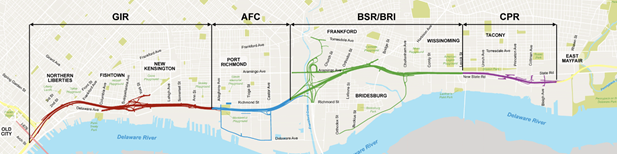
\includegraphics[width=0.8\textwidth]{gfx/chapter-introduction/i95revive_map.png}
	\caption[I-95 Girard Avenue Interchange Stormwater Project.]{I-95 Girard Avenue Interchange Stormwater Project map (PennDOT, 2018).}
	\label{fig:revive-full-map}
\end{figure}

\begin{figure}[ht]
	\centering
	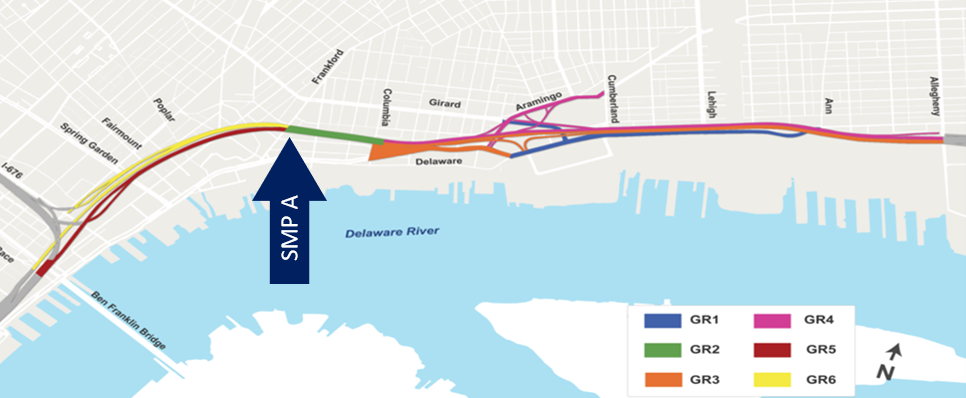
\includegraphics[width=0.8\textwidth]{gfx/chapter-introduction/gr2_map.png}
	\caption[I-95 Girard Avenue Interchange Stormwater Project GIR-GR2 Section.]{I-95 Girard Avenue Interchange Stormwater Project GIR-GR2 section map (PennDOT, 2018).}
	\label{fig:GR2-map}
\end{figure}

SMP A is a linear bioinfiltration type garden nearly 100m in length but only 10-12m wide due to tight urban geometry constraining the site.
Infiltration occurs in over 80\% of the garden, with just a small portion in the center lined to protect neighboring structures.
To better understand the site's hydraulic performance, monitoring equipment was installed in mid-2017 to quantify volume and soil state, and aid in the development of an EPA Stormwater Management Model (SWMM) by former Villanova Center for Resilient Water Systems graduate Elizabeth Calt (\citeyear{Calt2018}).
Further work has been undertaken to improve the monitoring network's reliability and accuracy.
This site is funded by PennDOT through the AECOM University partners program with the goal of investigating the long term performance of GSI as a stormwater management tool.

\section{Research Goals}
The primary goal of this work is to identify multi-faceted strategies for improved long-term monitoring solutions that will enable more thorough analysis of GSI.
The steps outlined in the following chapters are intended to provide insight to PennDOT, AECOM, and their project partners in the continued study of wide-scale GSI projects on the I-95 Girard Avenue Interchange Stormwater Project, as well as to other partners in the city of Philadelphia who seek to expand GSI systems to the watershed scale and beyond.
The creation of more uniform monitoring and long-term analysis practices will help move the design of GSI towards practices that are longer lasting, easier to maintain, and less prone to construction errors or failure.
The steps outlined include three separate facets:
\begin{itemize}
	\item The use of digital sensors with more accurate sensing and data transmission makes continuous monitoring more reliable and less prone to unrecoverable errors.
	\item Storing data in a flexible schema, such as the Stormwater Infrastructure Data Model in use at Villanova, enables long term study and comparison of a multitude of GSI locations.
	\item Event statistics generated from continuous monitoring data, such as recession rate and soil drying rate, can be used to approximate more labor-intensive field and lab tests to ensure continued performance.
\end{itemize}
Each of these topics will be discussed in detail in the following three chapters, with a focus on lessons learned through implementation at SMP A.


% !TEX root = ../main.tex
%
\chapter{Standardized Data Collection}
\label{sec:data-collection}


\section{Background}

In urbanized environments, the high percentage of surface area covered in impermeable asphalt or buildings causes increased runoff and reduced evaporation and infiltration (Figure \ref{fig:urban-water-budget}).
Urban environments have long faced challenges when it comes to handling this increased runoff in a ecologically friendly manner that avoids disastrous flooding while also minimizing the impact to stream and river health from pollutants and erosive flow rates.
As cities' impervious footprints grow, sewer networks have became overwhelmed by the volumes seen during storm events, and outfall locations were added to avoid sewage backup into homes and streets.
In Philadelphia, combined sewer systems (CSS)  were the preferred method of handling large volumes of rainfall and sewage for nearly the city's entire history (\cite{Akhavan2015}), but have a major negative impact on the environment via combined sewer overflows (CSO).
The EPA's oversight of CSO events, outlined in the Clean Water Act of 1972 and regulated by the National Pollutant Discharge Elimination System (NPDES) permit program (\cite{USEPA2009}), require that cities address urban runoff and impose significant fines for overflow events.
Only recently have green initiatives such as Philadelphia's "Green City Clean Water" expanded, allowing the city to expedite the creation of environmentally friendly means of removing stormwater (\cite{PhiladelphiaWaterDepartment2018a, Callahan2019}).
These systems allow urban stormwater, which primarily falls on impervious surfaces and leads to increased runoff as compared to natural environments, to be captured and managed largely in place (\cite{Heffernan2016}) by a combination of green infrastructure methods including rain gardens, tree trenches, green roofs, and pervious concrete.
The type of system chosen for a particular site depends on existing site infrastructure (e.g., buried utilities, surrounding structures, etc.), grading, available space, and loading ratio (directly connected impervious area (DCIA) vs system footprint).

\begin{figure}[ht]
	\centering
	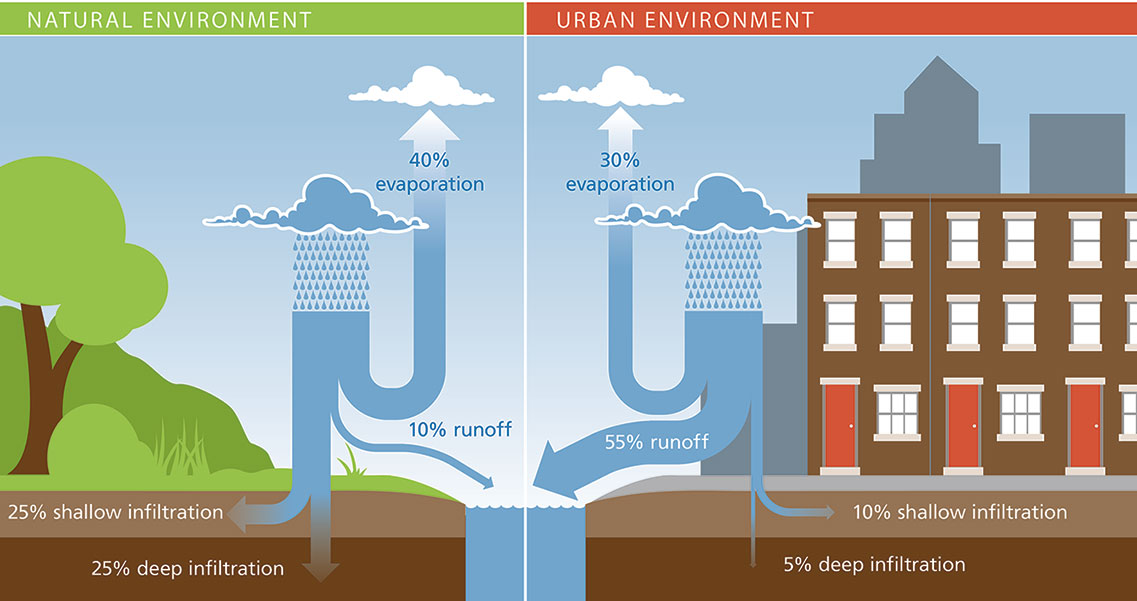
\includegraphics[width=0.8\textwidth]{gfx/chapter-instrumentation/naturalvsurbanrunoff.jpg}
	\caption[Natural vs Urban water budget.]{Natural vs Urban water budget (\cite{PhiladelphiaWaterDepartment2021}).}
	\label{fig:urban-water-budget}
\end{figure}

Measuring any natural or anthropogenic system is not without its challenges: atmospheric and physical parameters are subject to rapid change from weather patterns and equipment must be able to withstand harsh outdoor conditions for extended periods of time.
After all, nature obeys the laws of entropy, and energy tends to dissipate towards its lowest potential, and in doing so becomes a major force with which to be reckoned.
The water cycle that forms our climate is driven by solar heat inputs to this energy system.
Rainfall is generated from the accumulation of evaporated water in the atmosphere, which then condenses and falls to the ground.
Due to the randomness of entropy, no two storms will ever be the same in magnitude, duration, or intensity profile, so constructed solutions must be flexible enough to handle storms ranging from slow, drawn out events to short, intense events (\cite{Dourte2015, Maier2020}).

Collecting valid data is the first step to any rigorous experiment.
The methods used to collect this data must be reliable and easily repeatable for other parties who wish to replicate results.
That is to say identical inputs to a measurement system, given the same external conditions, should yield the same results.
This is a fundamental premise of the scientific method.
The most important aspects of monitoring a green stormwater infrastructure (GSI) system are a reliable data logger with minimal downtime, connected to a central data server (or "cloud") that collects data at a regular interval and redundantly stores that data for further analysis.
The data logger must be able to poll all connected sensors at timely intervals such that data measurements are associated with an accurate timestamp.
Measurements must be accurate, while their precision can be based on the unit of measure.
The ability to continuously monitor GSI conditions enables an understanding of design specifications versus real world performance.
While models are useful tools for understanding and managing expectations for GSI, they can only go so far at capturing real world knowledge and the many interactions of GSI conditions that create nearly endless combinations of unique conditions.

This chapter outlines a framework of best practices pertaining to the continuous remote sensing of GSI conditions developed for stormwater management practice (SMP) A in the GR2 section of the Pennsylvania Department of Transportation's (PennDOT) I-95 Girard Avenue Interchange Stormwater Project.
This framework has been developed to be reliable, consistent, easy to implement, and expandable to other GSI systems across Philadelphia with minimal additional configuration.
A primary goal of this research effort is to not only inform better data collection, but also to enable data to be collected at scale across many sites in a project or across many different projects.
A consistent, uniform framework for monitoring sites would allow for more widespread analysis of GSI's performance, maintenance needs, and impact on the natural environment (\cite{Burcin2014}).
This aligns well with the I-95 Girard Avenue Interchange Stormwater Project's long term horizon for construction, monitoring, and analysis of individual GSI systems and wider wholistic project or regional scale analysis.
A uniform approach across many individual sites ensures that statistical contrasts at the regional scale are accurate and unbiased.
To that end, measurements must be precise and data recording and transmission must be unhindered by the inherent randomness or other inconsistency of environmental systems.
Myriad challenges exist in monitoring GSI systems, but the focus of this discussion is accurate measurements of ponded and flowing water, which exhibits a wide variety of properties ranging from depth and velocity to random formations of currents and internal feedback in the form of turbulence (\cite{mays2010water}).
This monitoring framework has been established based on work performed at SMP A, a well developed and successfully performing GSI installation, for use across other PennDOT sites or for wider adoption across a regional scale in Philadelphia to enable long-term, meaningful comparisons of GSI performance across many systems.
The framework is intended as a basis for answering questions about ongoing maintenance requirements, identifying under-performing sites, and quantifying with high accuracy the environmental benefits of successful systems.

\section{Site Configuration}
Situated along the south side of Interstate 95 northbound, SMP A handles inflow from the elevated roadway surface's rainfall runoff that flows through a network of pipes beneath the highway.
Most of the DCIA lies in the northbound highway section, per LiDAR surveys conducted in 2017.
SMP A is a linear bioswale type rain garden split into three sections by two check dams placed at roughly the third points of the garden (Figure \ref{fig:site-layout}).

\begin{figure}[ht!]
	\centering
	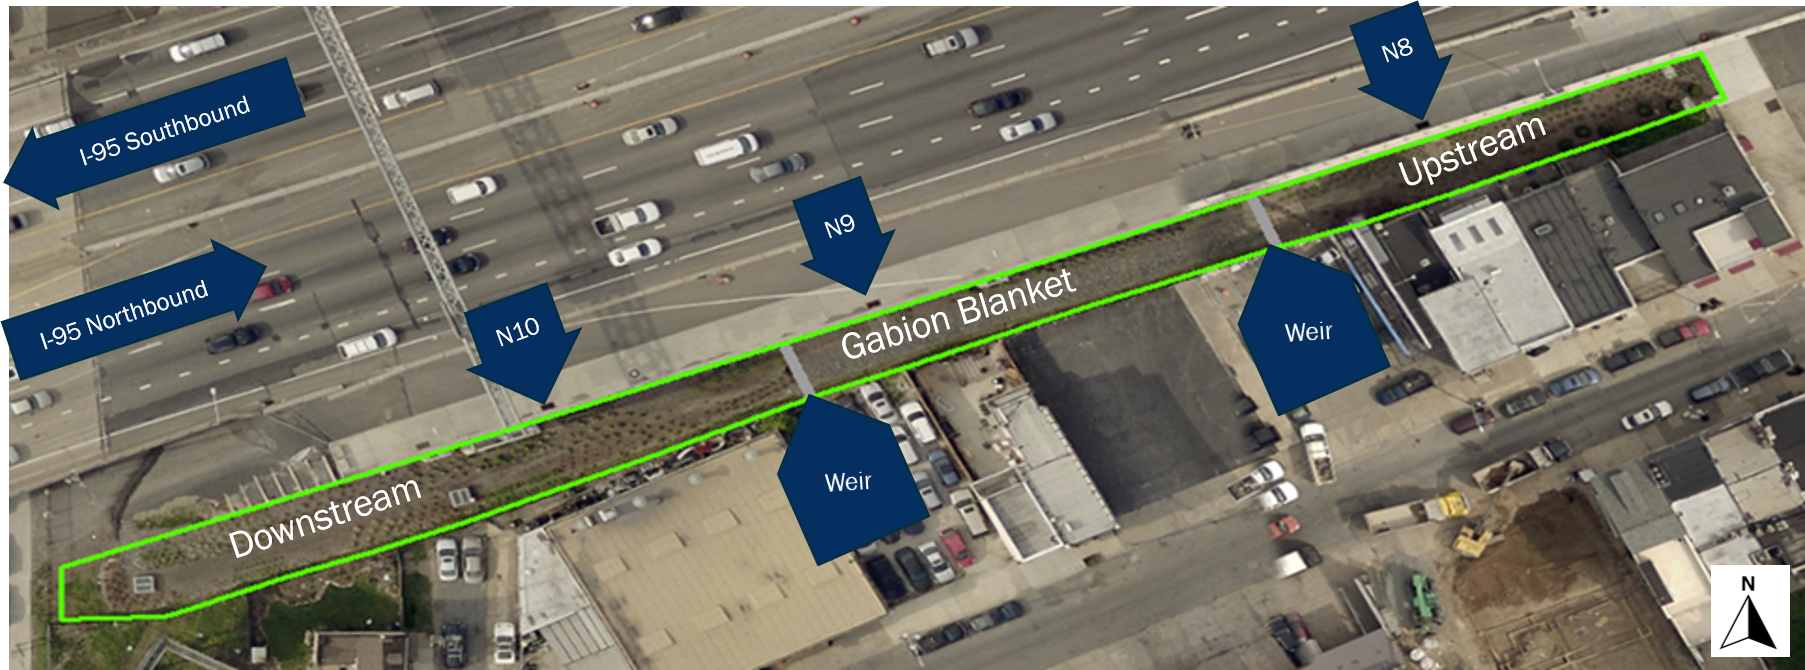
\includegraphics[width=0.8\textwidth]{gfx/chapter-instrumentation/site-layout.png}
	\caption{SMP A site layout.}
	\label{fig:site-layout}
\end{figure}

The upstream portion contains one inlet (N8) that is a 76.2cm diameter reinforced concrete pipe (RCP).
This upstream section is planted with local, salt tolerant grasses and small coniferous trees.
The surface is mulched during annual maintenance cycles, and the cross-sectional geometry is gently sloping (Figure \ref{fig:us-profile}).
The upstream section terminates with a 45\degree\ steel weir plate situated in the center of a plywood check dam that reduces flow rates, encourages infiltration by retaining some water, and measures inter-garden flow once overtopped using the standard weir equation (Figure \ref{fig:check-dam}).

\begin{figure}[ht!]
	\centering
	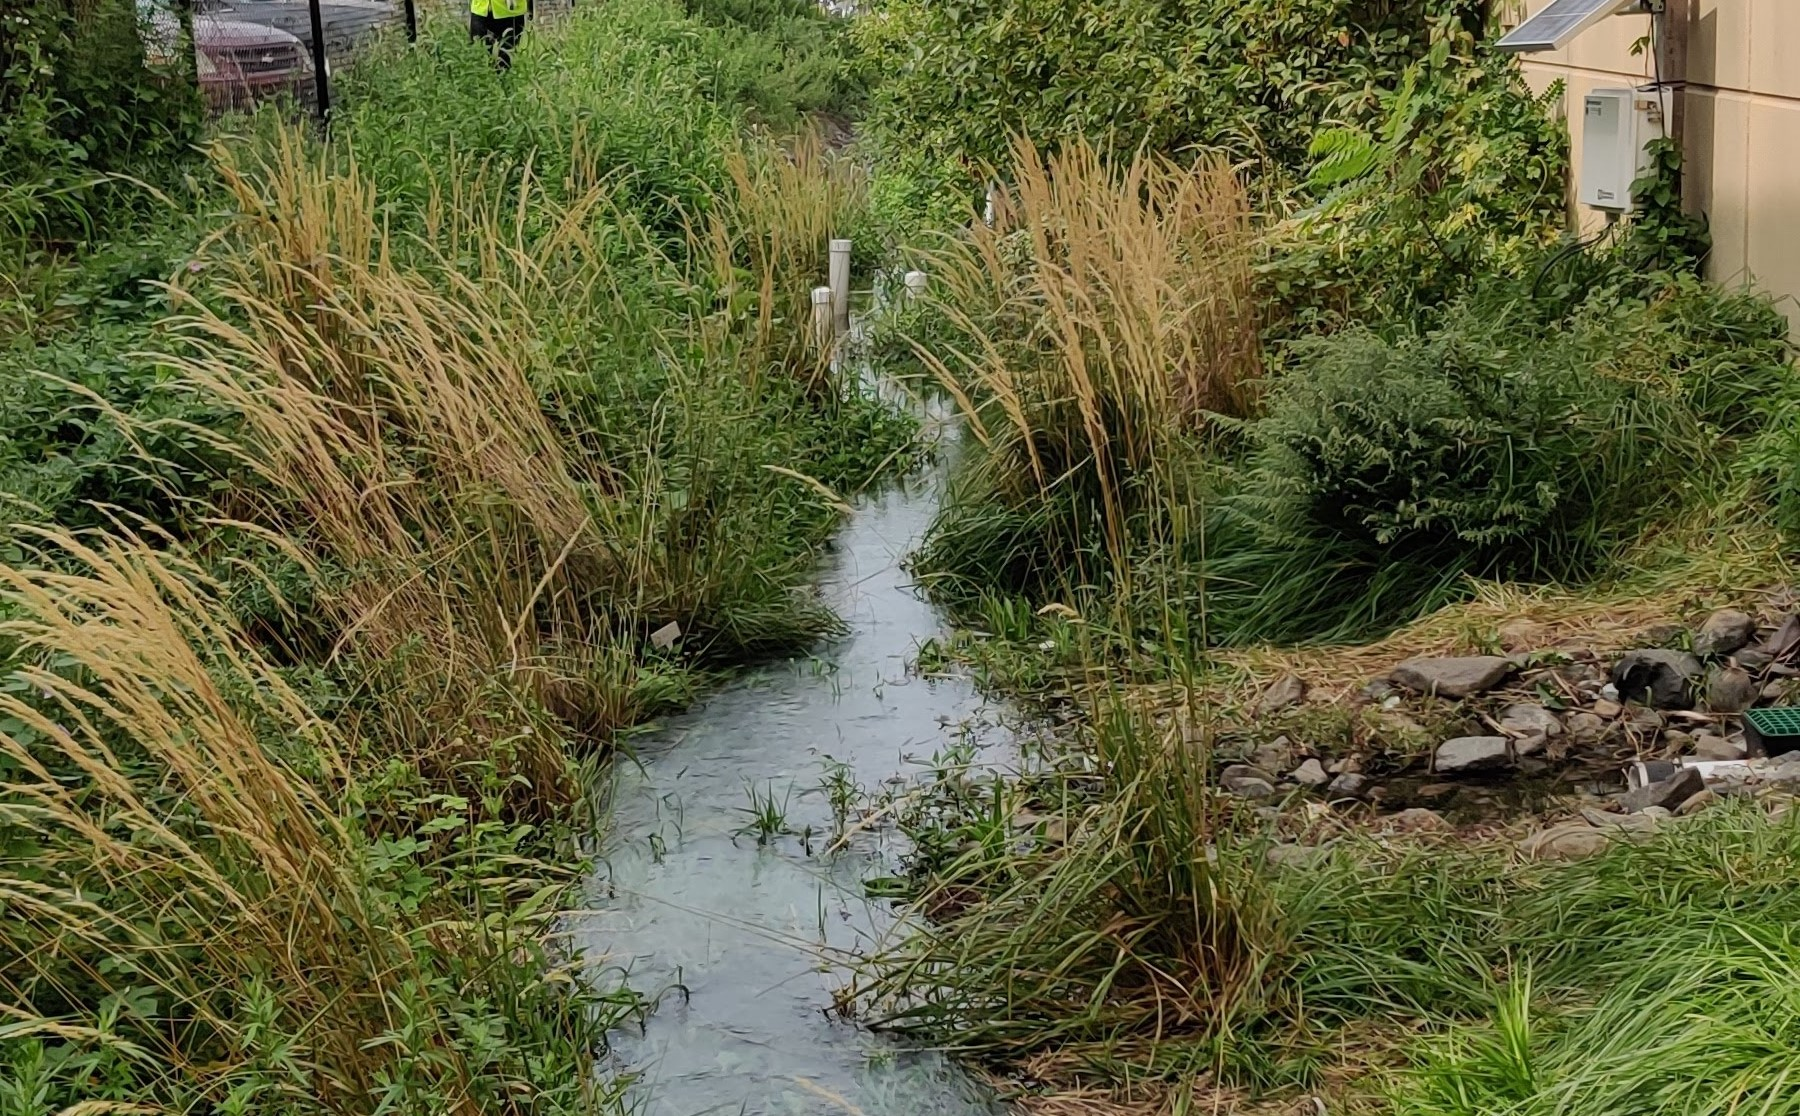
\includegraphics[width=0.4\textwidth]{gfx/chapter-instrumentation/smpa_upstream_profile.jpg}
	\caption[SMP A upstream profile during a simulated runoff test, September 2020.]{SMP A upstream profile during a simulated runoff test, September 2020. Note the shallow side slopes.}
	\label{fig:us-profile}
\end{figure}

\begin{figure}[ht!]
	\centering
	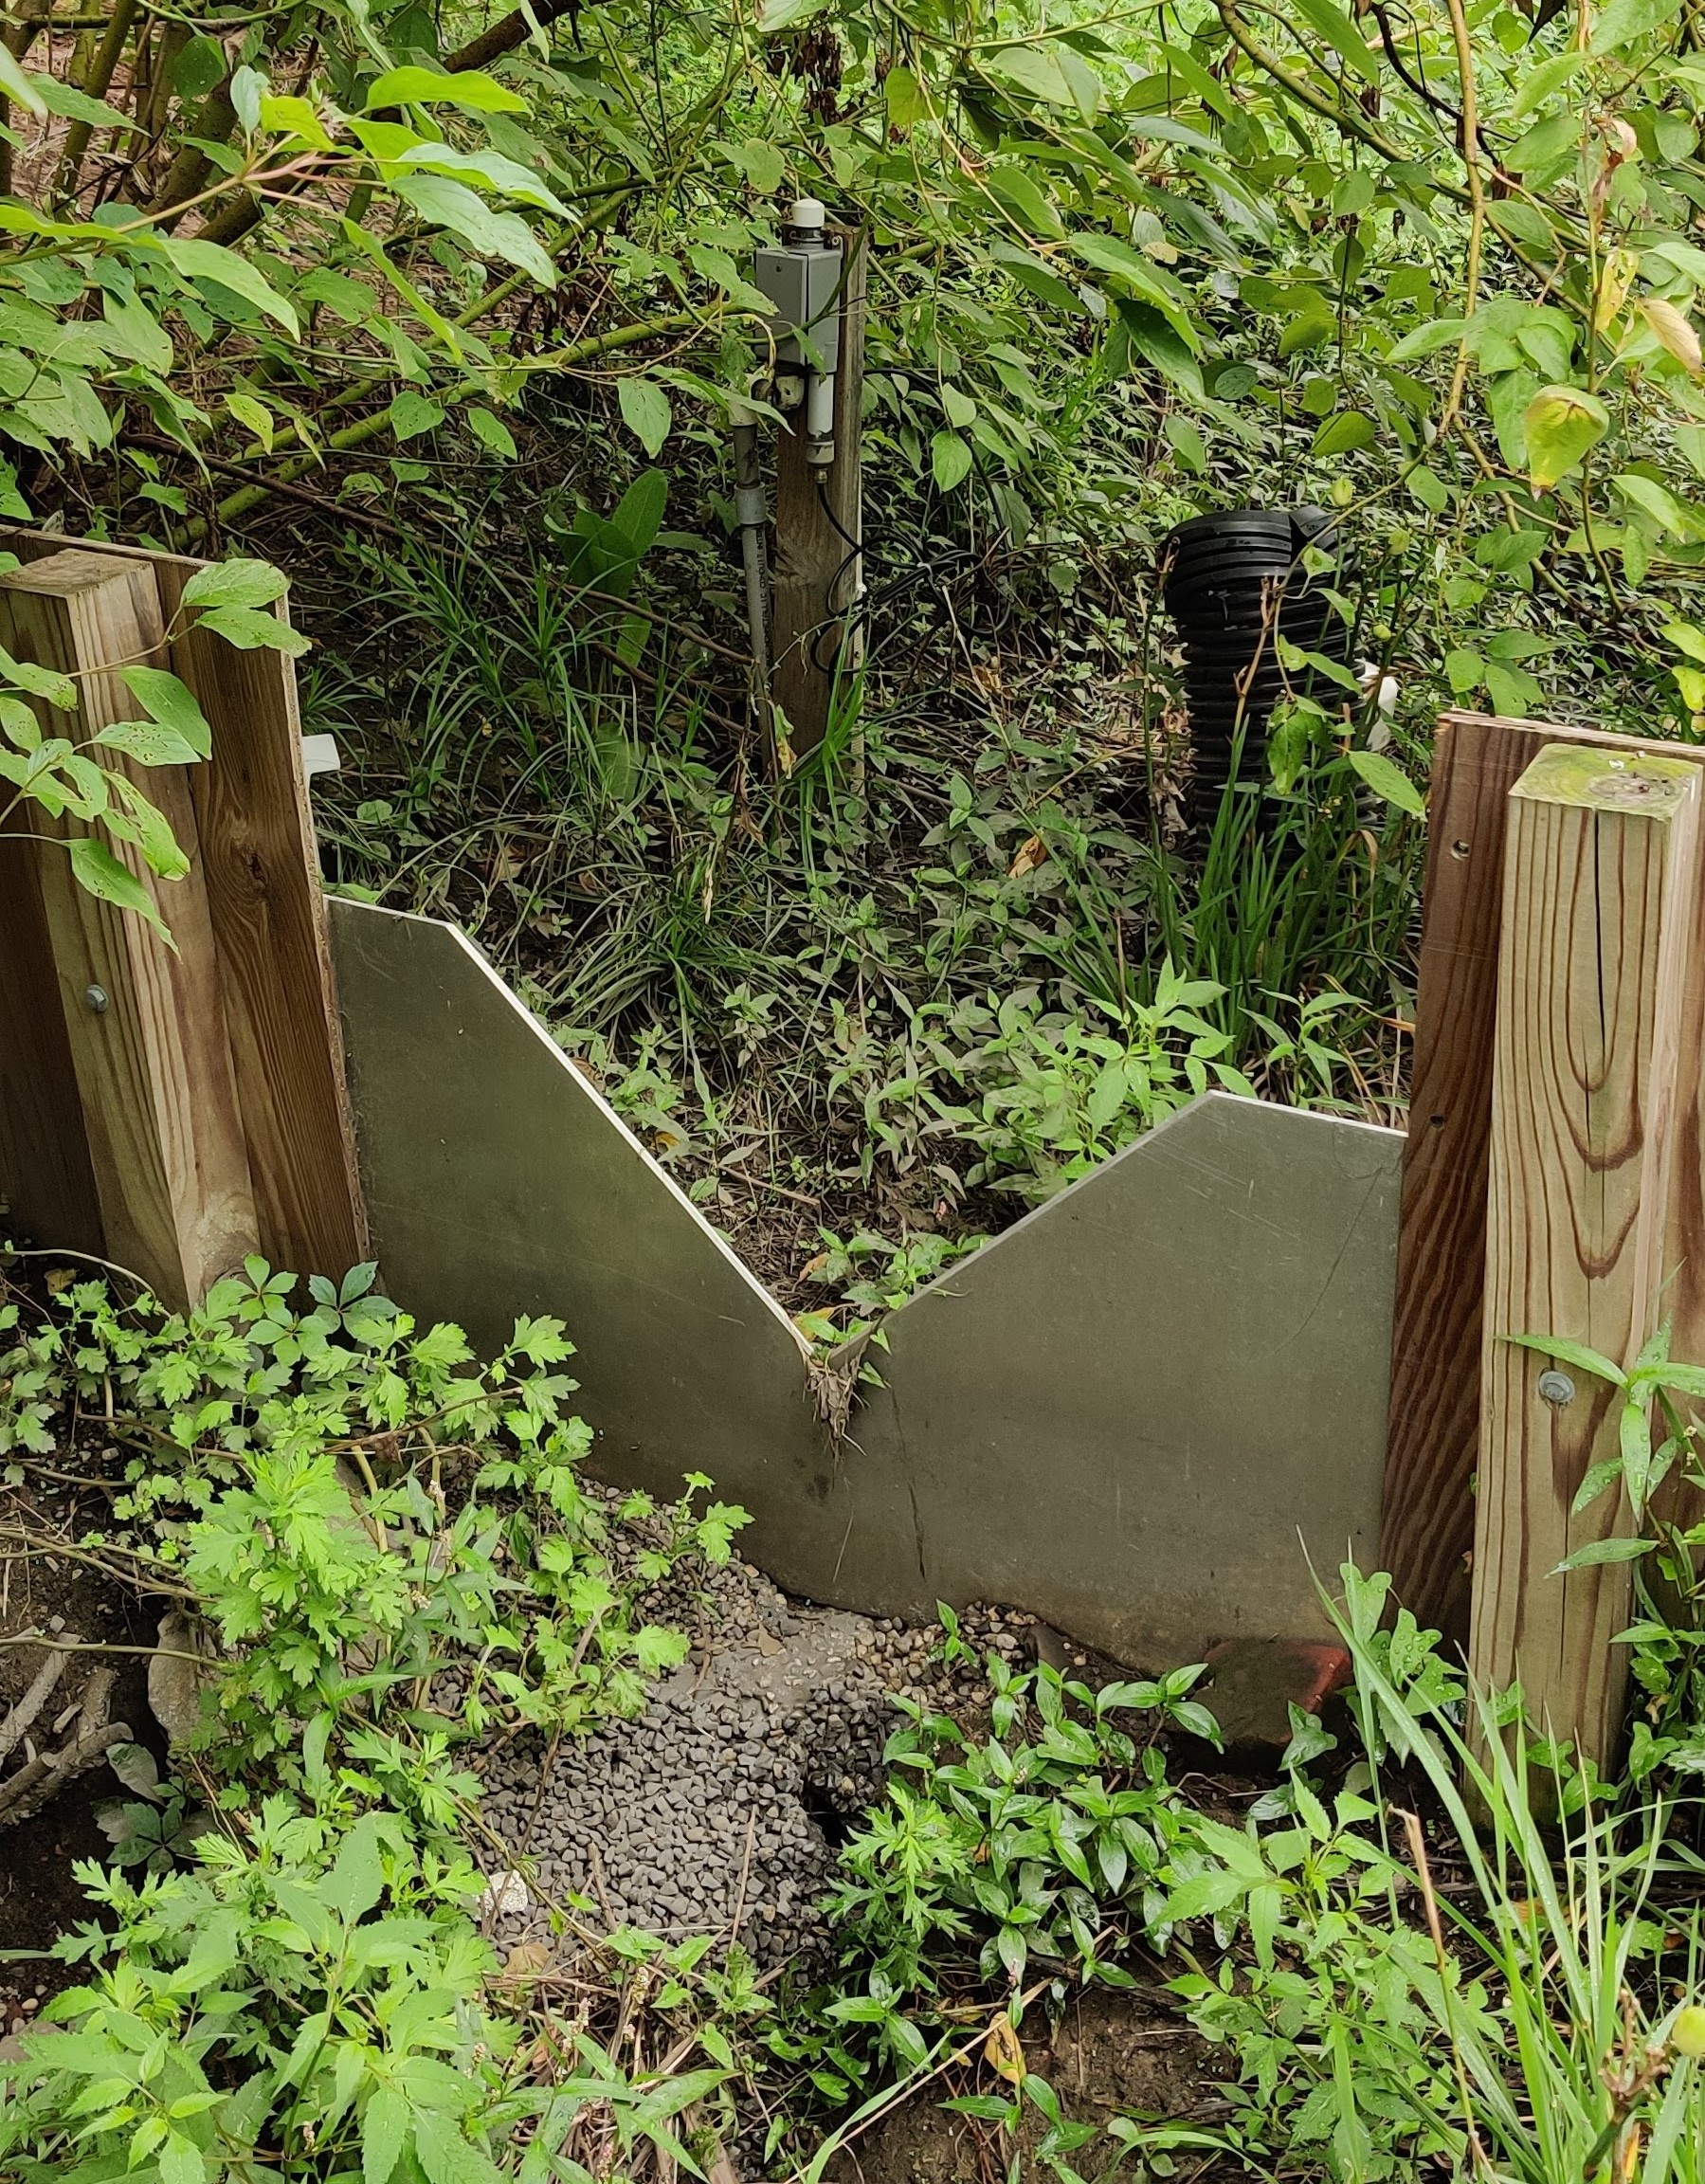
\includegraphics[width=0.4\textwidth]{gfx/chapter-instrumentation/check-dam-weir.jpg}
	\caption{Check dam at the downstream end of the central gabion blanket section of SMP A.}
	\label{fig:check-dam}
\end{figure}

The center section has an impermeable fabric beneath the entire south half of the section to prevent infiltration from damaging neighboring structures' foundations.
The entire section is constructed with gabion basket devices, which are intended to help prevent erosion and cut down on weed growth.
There is a single 45.7cm RCP inlet (N9) in this section and the cross section has more pronounced slopes (Figure \ref{fig:gabion-blanket}).
The gabion blanket section is similarly terminated at the downstream end by a 45\degree\ steel weir plate flush with a check dam to retain as much water as possible.

\begin{figure}[ht!]
	\centering
	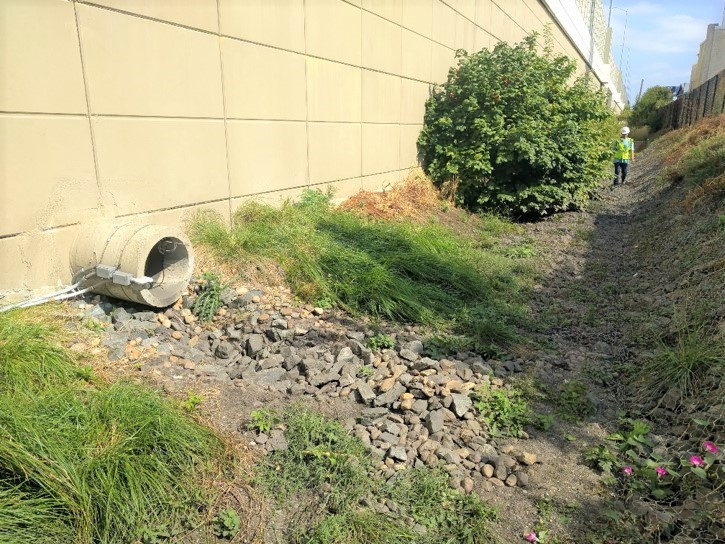
\includegraphics[width=0.6\textwidth]{gfx/chapter-instrumentation/gabion-blanket.jpg}
	\caption{Gabion blanket section showing highly sloped banks.}
	\label{fig:gabion-blanket}
\end{figure}

The downstream portion of the garden contains one more 45.7cm RCP inlet (N10), as well as two concrete overflow structures connected to Philadelphia's CSS identified as B1 and B2.
These structures have pressure transducer (PT) devices attached to the outside of the structure for measuring the ponded water level.
Inside the structures are 22.5\degree\ steel weir plates inside covering the CSS connection (Figure \ref{fig:outlet-structure}), with another pair of PT devices for measuring the outflow from the system, again using the standard weir equation.

\begin{figure}[ht!]
	\centering
	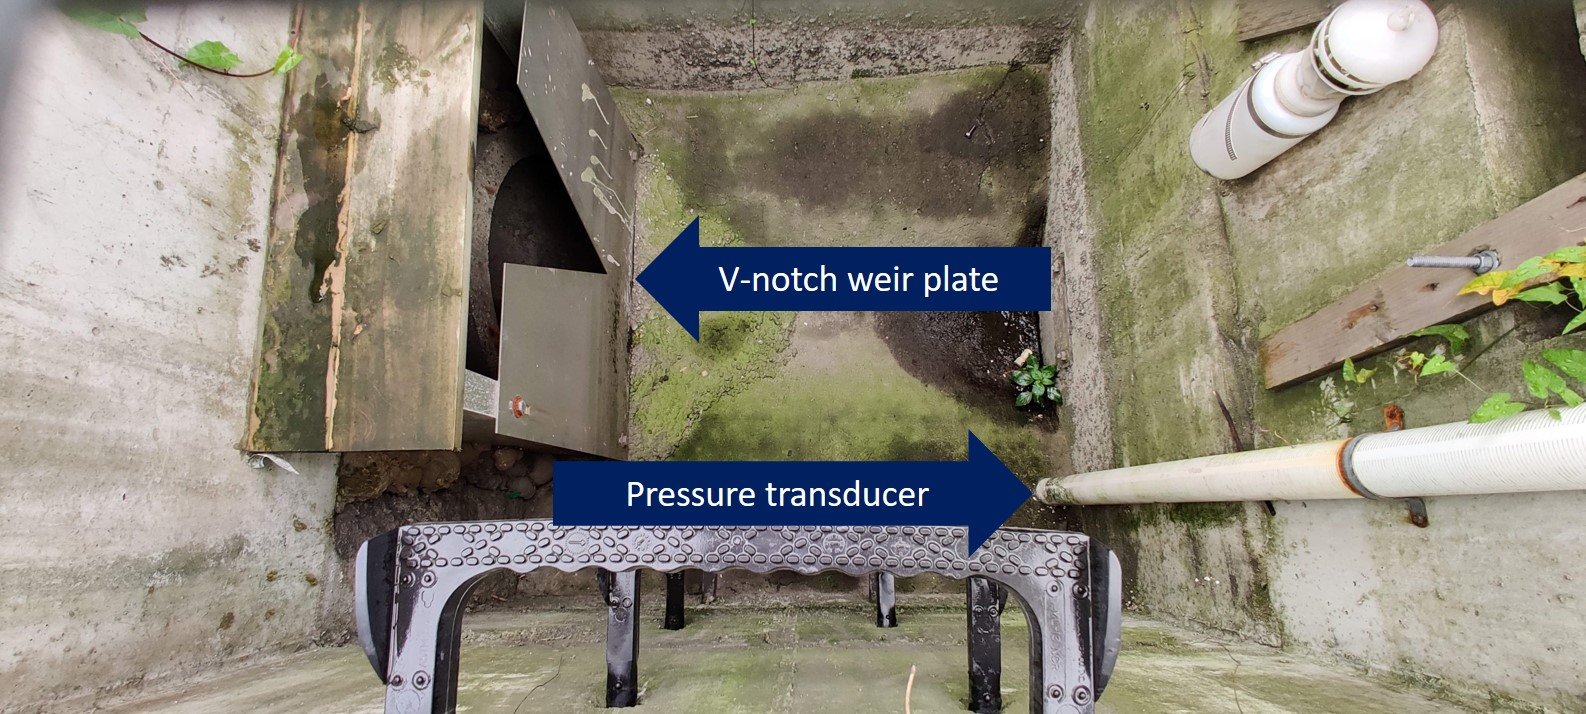
\includegraphics[width=0.8\textwidth]{gfx/chapter-instrumentation/b1-outlet-structure.jpg}
	\caption{B1 outlet structure with weir plate covering CSS connection.}
	\label{fig:outlet-structure}
\end{figure}

Due to SMP A's location at the border between the completed GR2 section of the project and the upcoming GR1 section to the west, there is a temporary construction ramp at the downstream end of the basin that leads from the elevated roadway to grade level adjacent to Frankford Ave.
The ramp is not intended to convey inflow, but the grade of the highway, misalignment of inlet grates (Figure \ref{fig:misaligned-catchments}) on the highway, and lack of barrier at the top of the ramp mean that a substantial amount of runoff enters the basin after flowing down the ramp.
All pressure transducers used at SMP A are a model CS451 digital pressure transducer from Campbell Scientific and are used in their SDI-12 communication mode.

\begin{figure}[ht!]
	\centering
	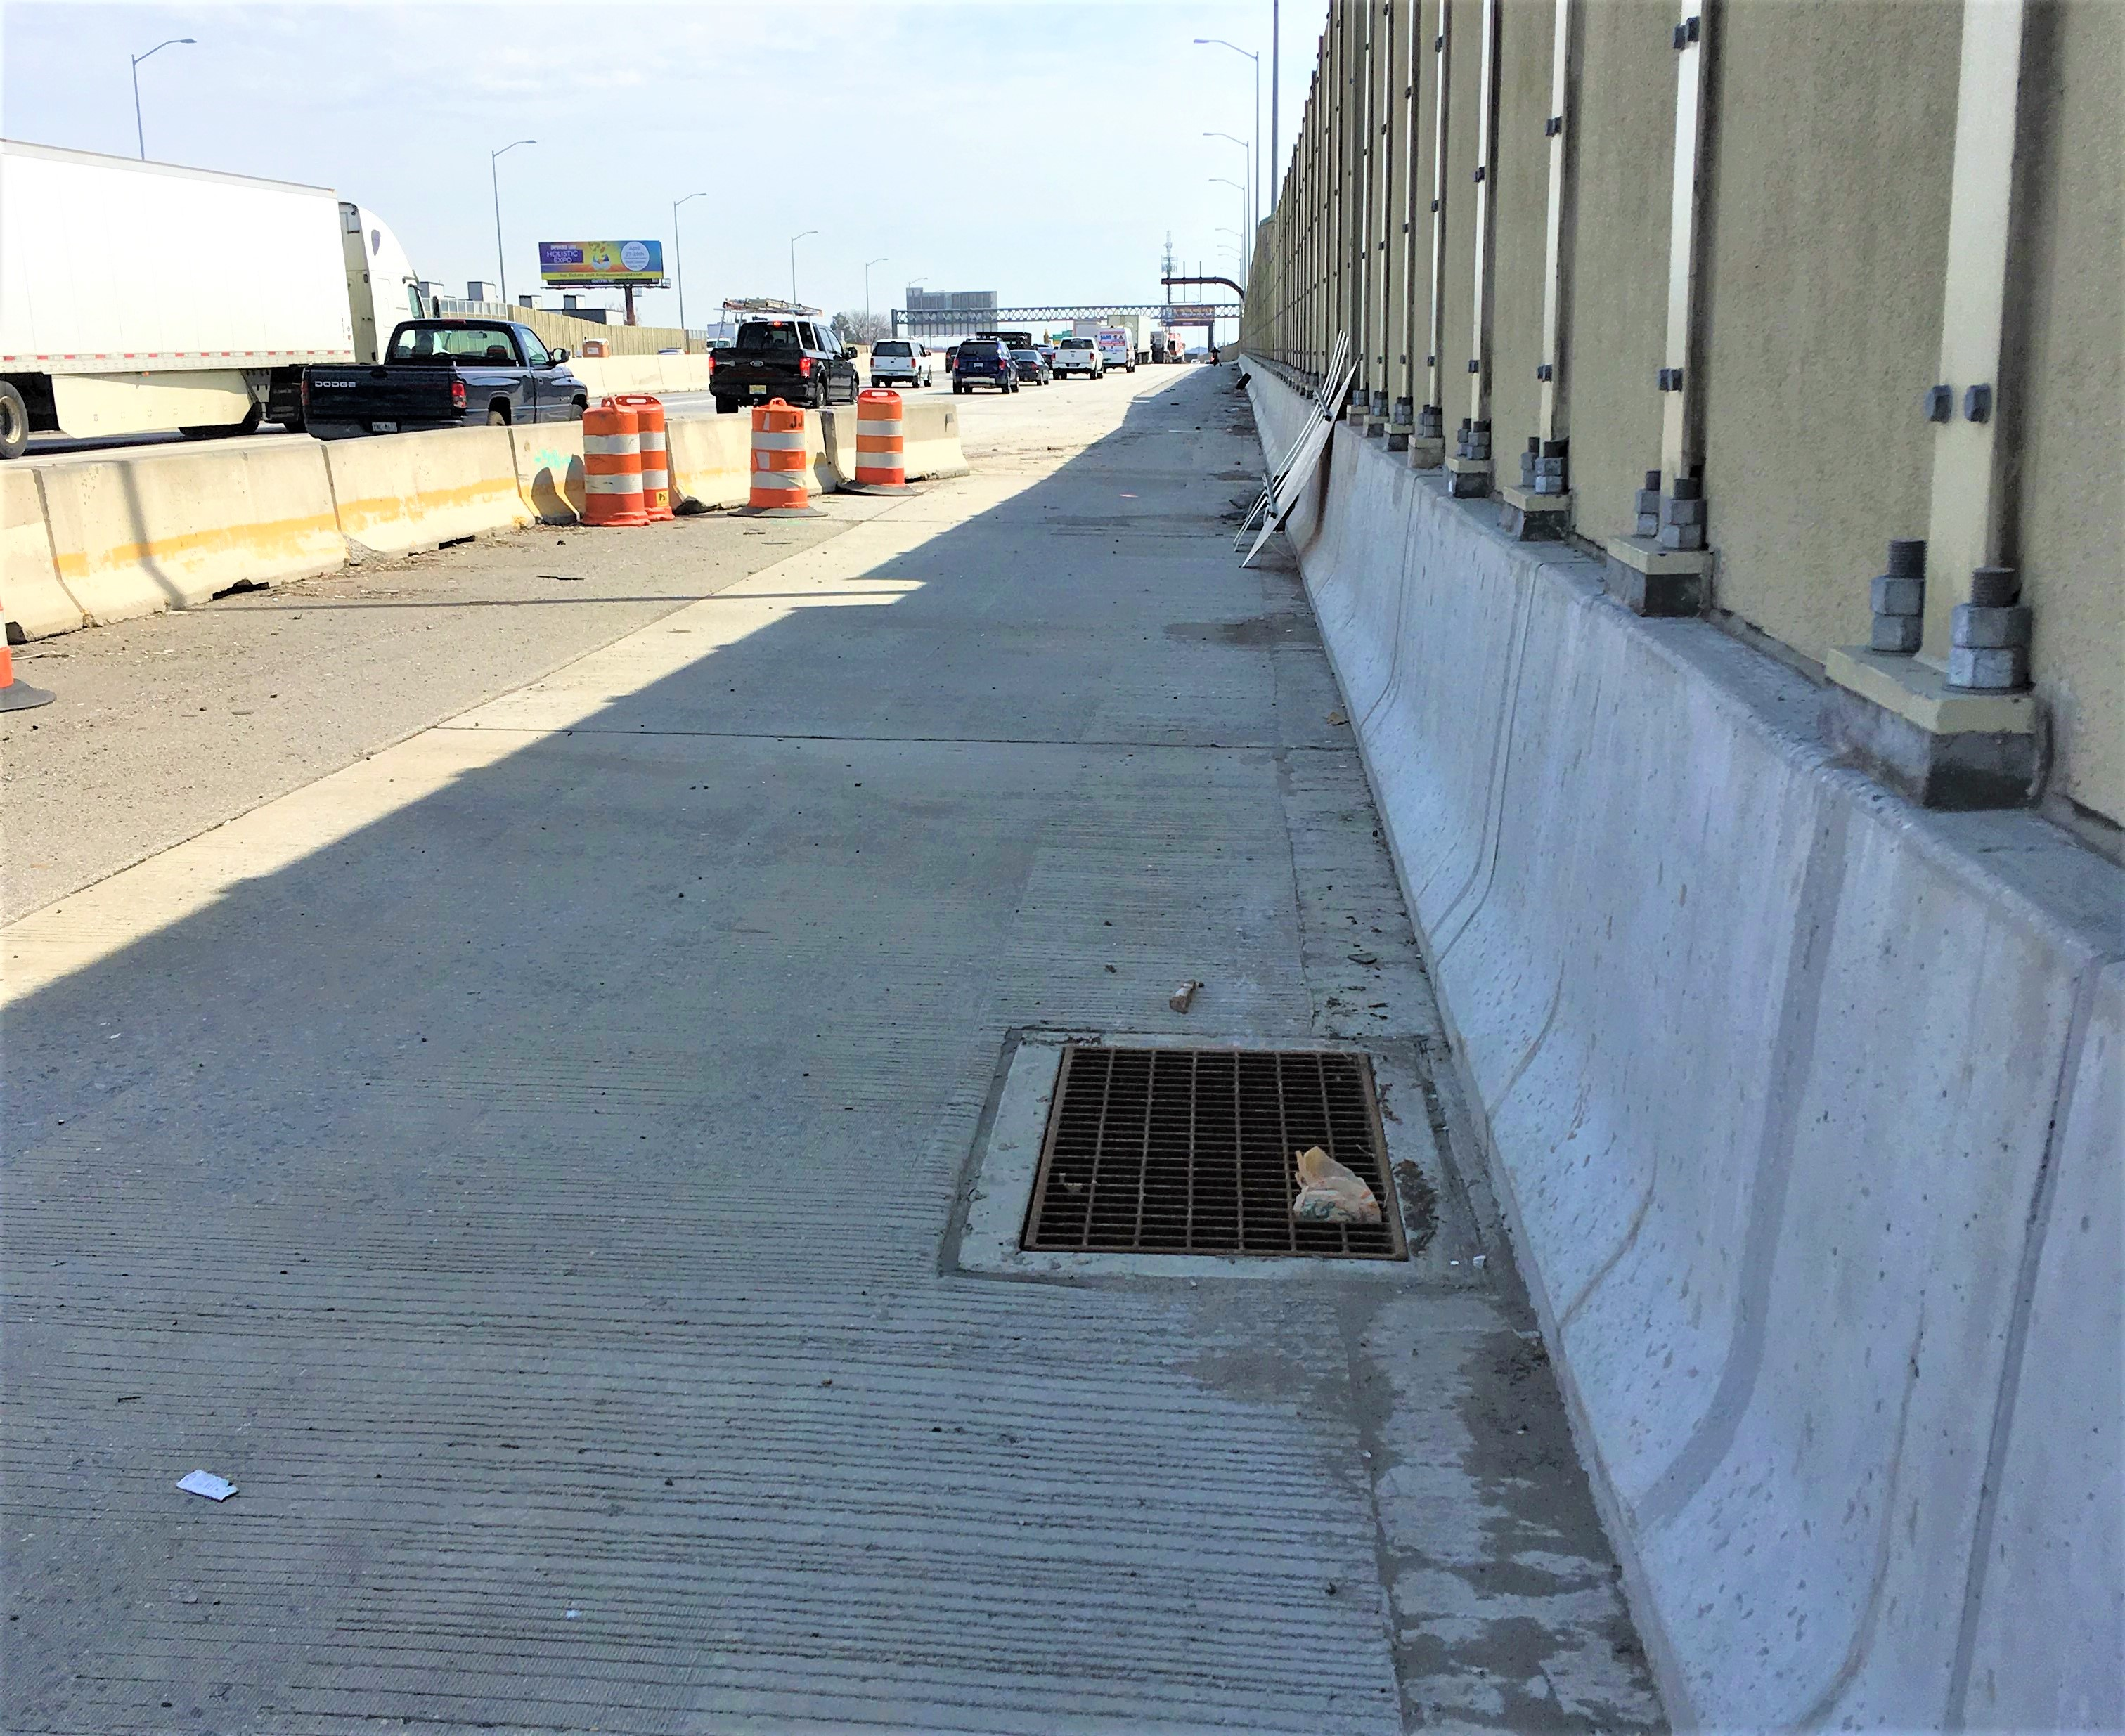
\includegraphics[width=0.6\textwidth]{gfx/chapter-instrumentation/misaligned-catchments.jpg}
	\caption{Misaligned inlet grates allow water to bypass and flow down the temporary ramp.}
	\label{fig:misaligned-catchments}
\end{figure}


\subsection{Measurement: Sensors and Structures}

To aid in repeatable, accurate, and timely measurements, sensors are deployed at a variety of locations throughout SMP A.
Pressure transducers in a variety of locations monitor both ponding level (outside the B1 and B2 outlet structures) and the depth behind weir plates (inside B1 and B2, and behind two check dams separating garden sections).
The flow rate over weir plates can be calculated using the standard weir equation (\cite{USBR2007}).

Inlet flow at N8, N9, and N10 was originally measured by a single BlueSiren Dual Wave Doppler Area-Velocity (AV) sensor at each inlet.
These sensors are fixed to expandable steel bands that secure the apparatus inside the end of the RCP by means of a screw jack.
Located at the downstream end of the AV sensor is a PT that measures flow depth, and outputs a 0-5V analog signal proportionate to the observed depth.
The voltage response must be calibrated with several known depths to establish a valid conversion equation (see section \ref{sec:challenges}).
At the upstream end of the AV sensor, the dual wave doppler measures flow velocity and outputs an 8-bit serial signal, with the number of doppler pulses reflected by the water corresponding to the velocity in millimeters per second.
Both parts of the AV sensor require 12V direct current (DC) power supply, which is managed by the CR6 data logger.

Soil moisture is measured at two locations using sensors at 10cm, 35cm, and 60cm depths, with an additional, redundant sensor at 35cm for quality assurance purposes.
Stevens Water Hydraprobe sensors (Figure \ref{fig:hydraprobe}) are used to measure soil moisture level, conductivity, resistivity, temperature, plus real and imaginary dielectric permittivity.
Hydraprobes use four stainless steel prongs to measure the soil's parameters and "take into account the energy storage and energy loss across the soil area using a 50MHz radio frequency wave" (\cite{StevensWater}).
The sensors are located in the middle of the downstream basin between outlet structures B1 and B2, as well as in the upstream basin approximately 2 meters from the check dam.

\begin{figure}[ht!]
	\centering
	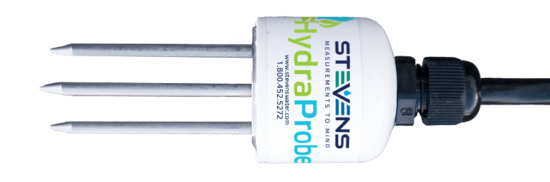
\includegraphics[width=0.6\textwidth]{gfx/chapter-instrumentation/hydraprobe.png}
	\caption[Steven's Water Hydraprobe.]{Stevens Water Hydraprobe (\cite{StevensWater}).}
	\label{fig:hydraprobe}
\end{figure}

Additional climate sensors include air temperature and relative humidity, solar radiation, wind speed and direction, and barometric pressure.
These sensors are located atop a 60-foot telephone pole adjacent to the I-95 bridge over Frankford Avenue that extends roughly 40 feet above the highway surface for measurements uninterrupted by traffic or highway structures.
These sensors are collectively referred to as the "Weather Station," and are a physically separate network from the main garden.

\subsection{Data Collection and Transmission}

The entire sensor network is controlled and monitored by three Campbell Scientific CR6 data logger devices.
These are located on poles attached to the B2 outlet, at the base of the weather station pole, and on a small post in the ground next to inlet N8.
The data loggers are inside protective boxes and have solar panels mounted adjacent to provide power and charge the 12V battery also located in each box.
The CR6 runs a program written in Campbell Scientific's CRBasic programming language, which is a procedural language similar to the BASIC family of languages.
The program defines variables, storage tables, polling and logging frequencies, and monitors the CR6's health and battery status.

Communications at SMP A are achieved via Campbell Scientific's Pakbus protocol, which allows multiple CR6 loggers at one site to be connected via external Wi-Fi modules (model NL240 and NL241) or RF devices (model RF407).
In early 2019, the existing RF devices were swapped out for Wi-Fi devices which improved range, reliability, data link speeds, and security.
Campbell Scientific LoggerNet software is used to remotely manage the data loggers, collect data every three hours, and identify issues that require on-site maintenance.

Remote connections are achieved via a Verizon 4G-LTE cellular modem which provides internet access for remote connections and download of data.
The modem is paired with the CR6 at the Weather Station, as this setup has the fewest instruments attached, and therefore the lowest power requirements.
Remote access is necessary for downloading data at a regular interval and monitoring the network's health.

There are four types of measurement performed by the CR6 data loggers: analog voltage difference, serial, pulse count, and digital.
Each have their advantages and disadvantages.

Analog voltage difference sensors, such as the BlueSiren AV depth reading, convert a 5V or 12V DC supply into a 0-5V response, which is read by the data logging device.
This method requires a calibration equation to translate the response voltage into meaningful units for the measured variable.
The reading is performed by the CR6 device and is almost always separated from the point of measurement (sensor) by a substantial length of wire (minimum 10m, maximum 90m).
Calibration is performed by applying a known reading to the sensor (depth of water in the case of a PT sensor), and recording the response voltage at several different readings.
A linear relationship (slope and intercept) are then calculated from the points collected, and this equation is written directly into the CR6 program.
Due to electrical resistance of copper wire varying with temperature (\cite{Eargle2002}), the resistance of a copper wire increases by 15\% over a 40\degree\ Celsius range when warmed by direct sunlight.
This is amplified by the long length of wire running between the sensors and data logger - nearly the entire 90-meter length of SMP A in some cases.
Change in resistance from the calibration condition is not compensated for by the CR6, so measurements made at temperatures different from the calibration temperature are subject to error.
Historically, wiring has been installed at least partially above ground, exposing it to sunlight which can cause swings in temperature.
Existing in-situ calibration procedures may help reduce this, but further study is warranted.

Serial sensors send pulses of electrical signals at a given voltage and baud rate.
The CR6 data logger reads these serial values by opening a serial buffer on the port a serial sensor is connected to and can respond to a wide variety of serial protocols and refresh rates.
The Blue Siren sensors used at SMP A communicate velocity via UART - TTL at a baud rate of 4800.
Serial communications are less prone to error or disturbance introduced by the transmitting wires but have limits on how far a valid signal will transmit.
Additionally, only one serial sensor can be active on any given data logger port at once, so some inlet AV sensors are connected to switched 12V power outputs on the CR6 to allow multiple sensors to share a single physical port.
This complicates both the physical wiring of the sensors at the site, as well as the code required to handle toggling the power state in coordination with taking measurements.
Additionally, it is unknown what effect this power cycling of the AV sensors has on their performance.

Pulse count communications are used primarily by rain gauges.
Measurement occurs when a specific event happens, such as the tip of a tipping rain gauge.
The sensor briefly connects the measurement port to ground, creating an electrical pulse that is detected by the CR6.
This means pulse count sensors are among the simplest in terms of wiring, as they require only a measurement and ground lead.

Finally, digital sensors, including the CS451 PT, Hydraprobes, pyranometer, and thermometer, use the SDI-12 protocol which allows up to 62 addressed sensors on a single communications port.
The SDI-12 protocol allows the CR6 to poll sensors for up-to-date data on demand, and read the results back nearly instantaneously.
The digital transmission of data eliminates the need to run separate communications cables for each sensor, and consolidates the ports used on a CR6 to just one for most applications.
Sensors are able to relay several measurements to the CR6 in an array of values without concerns surrounding wire length or environmental conditions.

\section{Challenges}
\label{sec:challenges}

Water flowing through pipes or across surfaces is affected by a variety of factors: slope, roughness, temperature, and geometry (\cite{mays2010water}).
The slightest imperfections in the surface or inconsistencies in the roughness can introduce turbulence, a non-uniform flow regime not well suited to measurement by sensors best suited for steady, uniform conditions.
The act of falling from highway level to ground level, where measurement takes place, means that water has a high amount of kinetic energy and is thus more likely to splash around, disturbing calmer water and imparting some of its energy.
Turbulence is best handled by some form of flow straightener, calming device, or impoundment behind a flow-control device such as a weir plate that uses temporarily stored water to remove energy from incoming water.
At lower flow rates, this can also be accomplished through the use of high permeability foam, which has the added benefit of filtering out larger debris particles washed in from the highway surface.

Attempts to characterize the "average" storm year have been successful (\cite{Albright2018}) and provide a means of estimating rainfall over a given period of interest.
This rainfall can be used as the input for a system model, such as was created by Elizabeth Calt, MSCE `18 (\cite{Calt2018}).
The Environmental Protection Agency's (EPA) Stormwater Management Model (SWMM) created by Calt estimates runoff, storage, and overflow volumes and was used to estimate the expected values for the sensors measuring flow through the three RCP inlets during both historical rainfall records, and two design storms (2 year, 24 hour and 10 year, 24 hour).

Historical data from inlet N8, N9, and N10 show that the depth portion of the AV sensors is frequently negative, which is indicative of improper calibration or sensor malfunction.
Despite sensors regularly being calibrated carefully, and returning valid measurements immediately after calibration, measurement drift continues to be an issue.
Little of the data in the period of study is valid, with many negative values occurring during storm events, so the best estimates of inflow rates are from the aforementioned SWMM model developed by Elizabeth Calt.
In addition to negative inflow rates being invalid, the model suggests that flow rates lower than what the Blue Siren AV sensors are capable of detecting may occur frequently, depending on the size and shape of the runoff hydrograph.

Finally, the calibration procedure for existing Blue Siren AV sensors is both tricky to perform and subjective based on human error.
After removing the sensor from the steel band holding it inside the pipe, the sensor is submerged in a five-gallon bucket with water measured by hand to the nearest millimeter.
Simultaneously, the data logger program must be updated to read out the raw voltage received, and these values are recorded in an Excel spreadsheet.
After taking measurements at several depths, typically ranging from 25-150mm, the hand measured depths and corresponding voltages are transformed into a simple linear relationship (slope and intercept), which is then updated and enabled in the data logger's program.
While little to no drift over time is noticeable in historical calibration records, there is some oscillation that occurs do to the imprecision of human measurement during the calibration process.


\section{Solutions}

\subsection{Temporary Ramp}

In June 2019, approximately 60 sandbags were added to an existing asphalt berm on the ramp.
These sandbags were placed to guide water through an 0.8-foot (20.32cm) H-flume with a PT sensor to capture the hydraulics of the ramp (Figure \ref{fig:temporary-ramp}, \cite{OpenChannelFlow2021}).
The flume is sourced from OpenChannelFlow, a company in Boise, ID that focuses on agricultural flow measurement devices.

\begin{figure}[ht!]
	\centering
	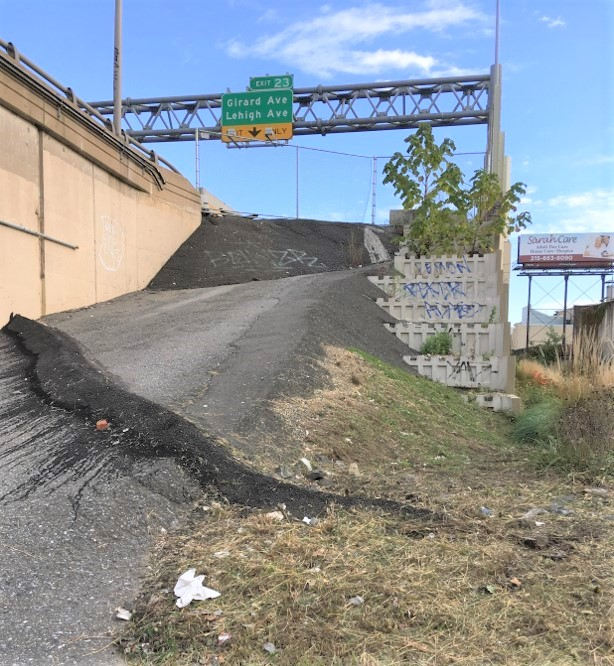
\includegraphics[width=0.6\textwidth]{gfx/chapter-instrumentation/temporary-ramp.jpg}
	\caption{Temporary ramp at the downstream end of SMP A.}
	\label{fig:temporary-ramp}
\end{figure}

The addition of the H-flume near the B1 outlet structure was driven by a desire for better understanding of hydraulic inputs to the basin that were bypassing storm drains on the roadway surface and instead flowing down the temporary ramp.
The H-flume is made of reinforced fiberglass and is sized based on preliminary output from Elizabeth Calt's SWMM model using both design storms and historical rainfall data collected at the site through early 2019.
It has a 1-meter (3-foot) approach section, and two cylindrical measurement wells on either side of the pour point which are 150mm deep (Figure \ref{fig:flume-drawing}).
Using the known offset of these wells, the data recorded by a CS451 PT can be used along with the calibration curve supplied by OpenChannelFlow to establish the flow rates observed:

\begin{equation}
	F = -0.00707921 + 0.04898248\ d^{0.5} + 21.70307374\ d^{1.5} + 365.9132927\ d^{2.5}
\end{equation}

where F is flow in liters per second and d is depth of flow in meters, which gives this flume a range of 0.0085 - 12.94 L/s (\cite{OpenChannelFlow2021}).
Flumes have long been an agriculture industry standard for measuring flows into and out of fields and ponds, and they are well equipped to handle a large range of flow rates.
While the sandbag wall has been tampered with on several occasions, it largely remains intact and able to direct water through the flume (Figure \ref{fig:flume-site-1}).
Only minor leakage was observed during a fall 2020 simulated runoff test (SRT) when a high flow rate was pumped into the site.

\begin{figure}[ht!]
	\centering
	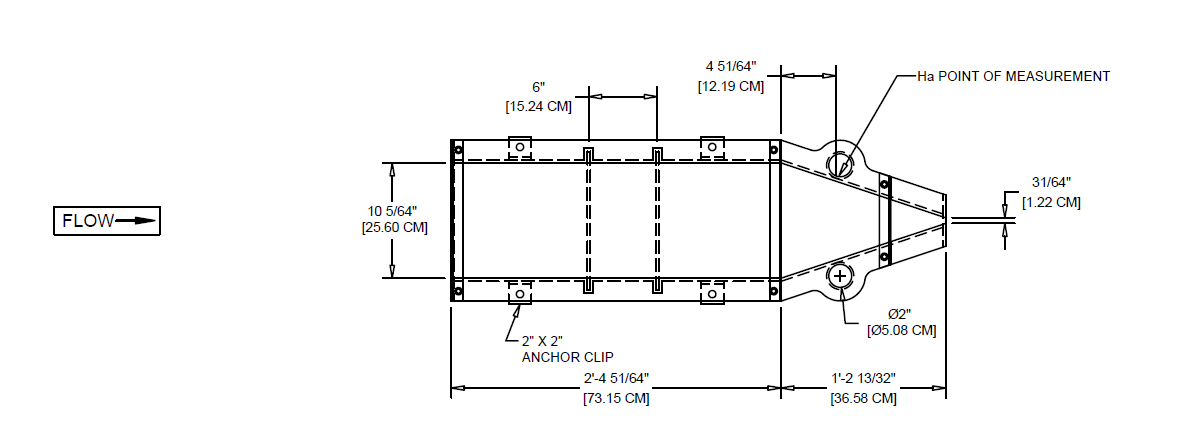
\includegraphics[width=0.8\textwidth]{gfx/chapter-instrumentation/h-flume-plan-view.png}
	\caption[0.8-foot OpenChannelFlow flume plan view.]{0.8-foot OpenChannelFlow flume plan view (\cite{OpenChannelFlow2021}).}
	\label{fig:flume-drawing}
\end{figure}
\begin{figure}[ht!]
	\centering
	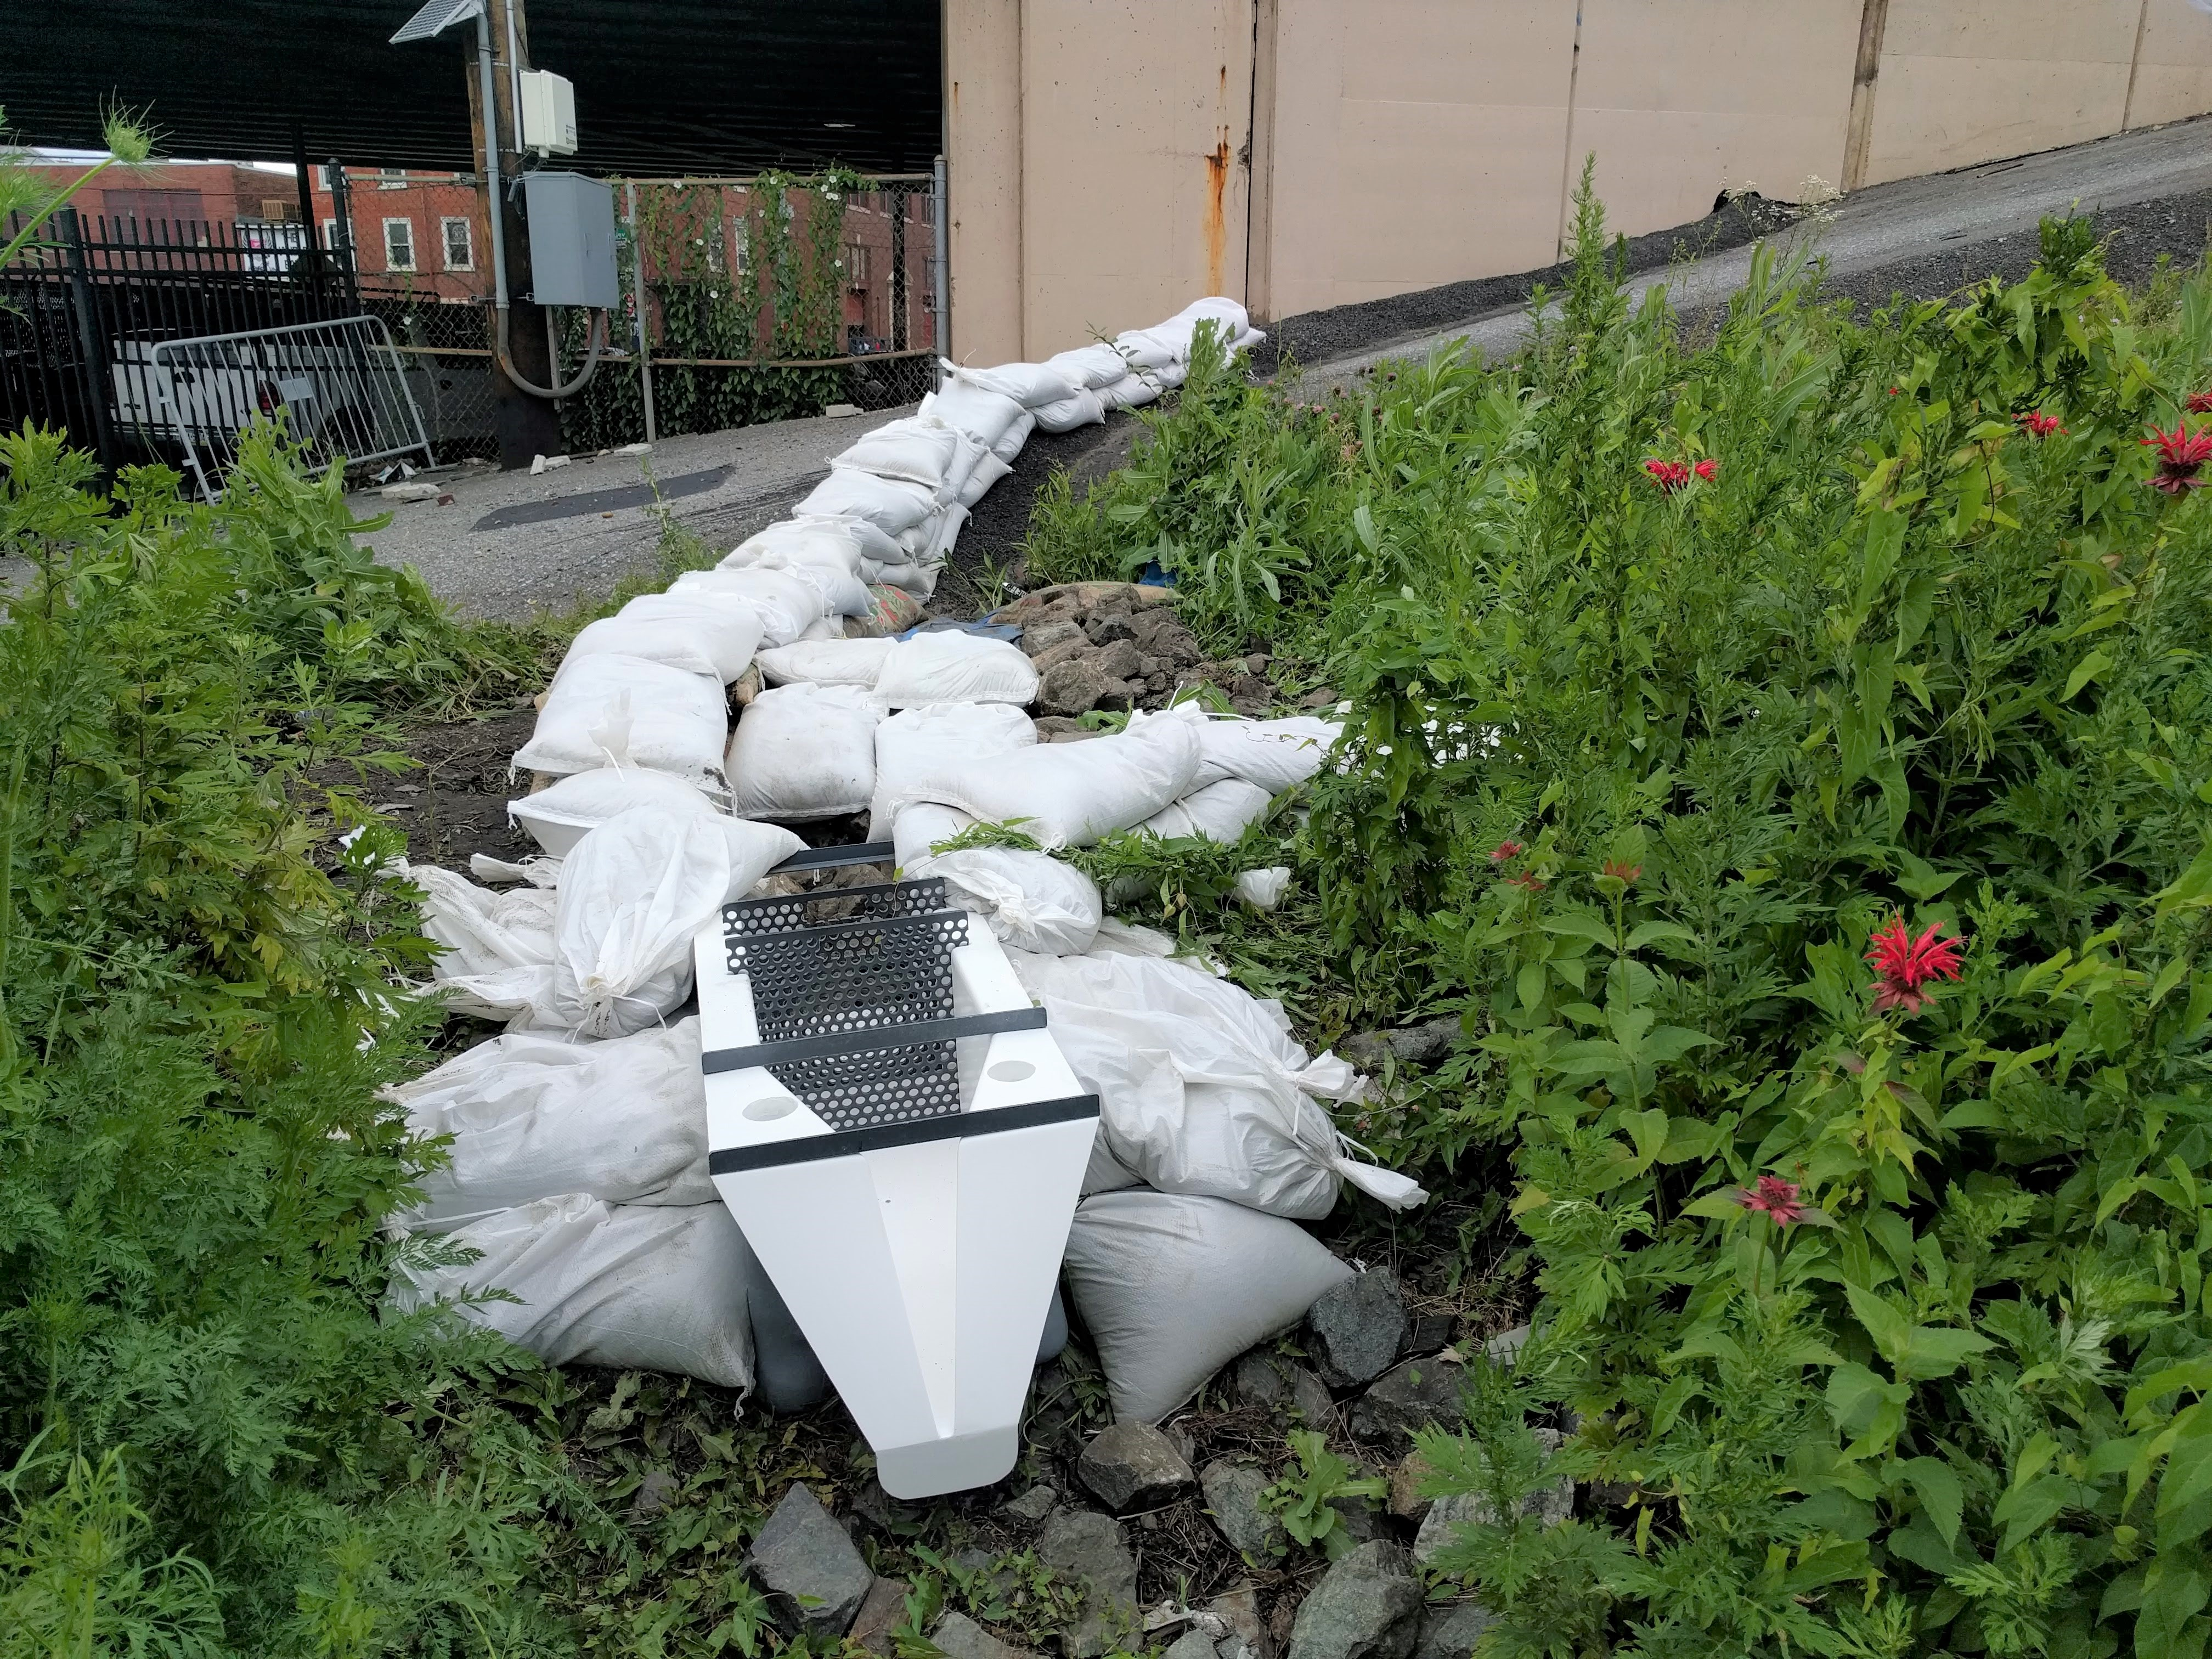
\includegraphics[width=0.6\textwidth]{gfx/chapter-instrumentation/flume-install.jpg}
	\caption{Flume installation at the bottom of construction ramp, 2019.}
	\label{fig:flume-site-1}
\end{figure}

\subsection{Inlet Flow Measurement}

To estimate the AV sensors' range, a suite of tests were performed using a lab simulation of field conditions.
Sensors were attached to an identical steel band and placed inside a 20cm PVC pipe.
The roughness of the pipe is different than that of the RCP installed in SMP A.
However, given the turbulence introduced by the flow falling from highway level to ground level a short distance upstream of the measurement point, roughness does not control the flow profile (\cite{mays2010water}).

The lower bound for Blue Siren AV sensors was determined in Villanova's water resources lab by calibrating a sensor using the same procedures used in the field, and then recording the sensor output and flume flow rate simultaneously.
Analysis showed (Figure \ref{fig:av-lab-results}) that the AV sensors are not valid below 4.5L/s in the 20cm test pipe.
This deviation was found to occur separately in depth and velocity readings around an average of approximately 25mm depth and approximately 30mm/s velocity, which equates to 0.1 L/s in a 45.7cm pipe (N9, N10) or 0.14 L/s in a 76.2cm pipe (N8), although it was not possible to test flow rates this low in the lab.
A second Blue Siren system consisting of a serial ultrasonic depth sensor mounted to the top of the pipe combined with a "microvelocity" sensor that has a lower profile than the current Dual Wave doppler AV sensor was tested in an identical fashion and found to have lower velocity accuracy, but consistently better depth accuracy.
Figure \ref{fig:av-lab-results} compares the two Area-Velocity measurement methods, with the insert at right showing both systems measuring significantly lower than the reference flow rate.
\begin{figure}[ht!]
	\centering
	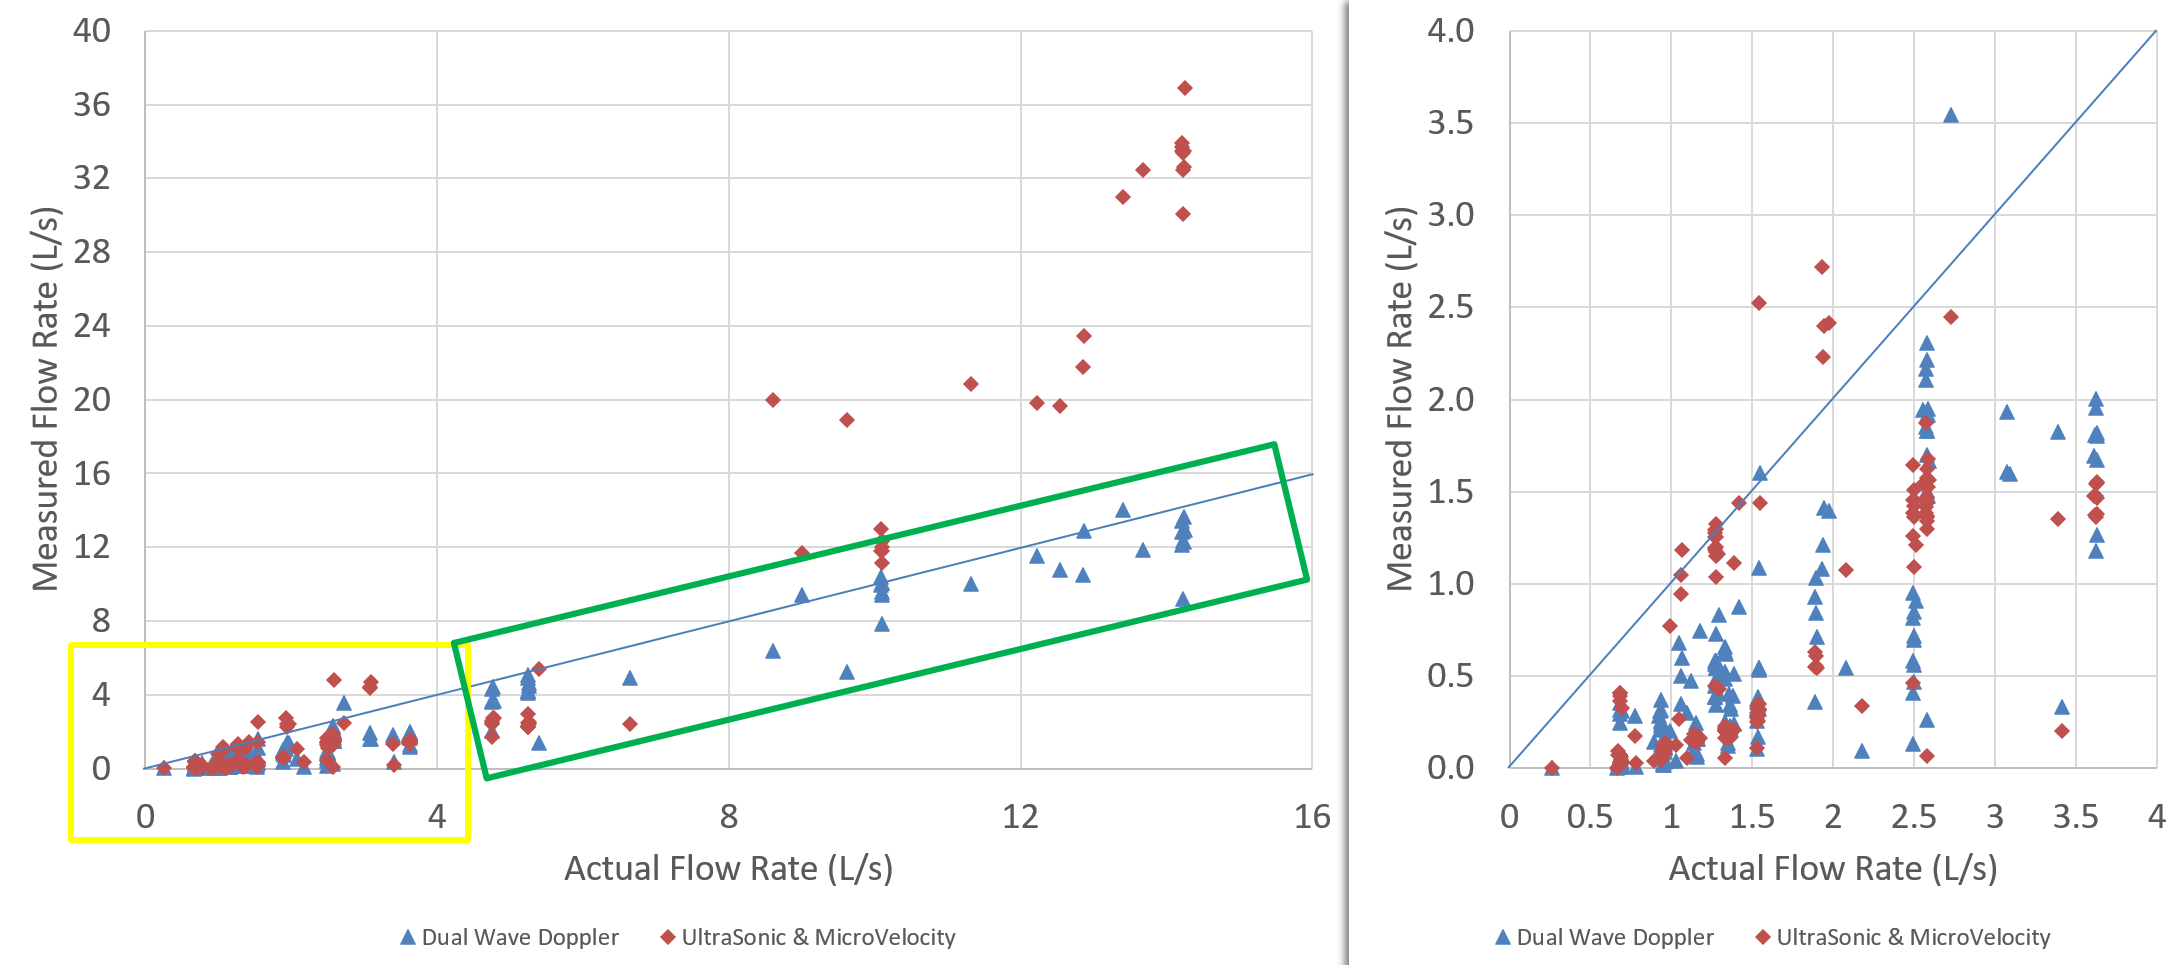
\includegraphics[width=0.8\textwidth]{gfx/chapter-instrumentation/AV-lab-results.png}
	\caption{Area-Velocity measurement comparison results.}
	\label{fig:av-lab-results}
\end{figure}

In order to capture lower flow rates, a restricting structure such as a weir plate or flume is necessary, so that the flow is forced through a narrower opening where it can be measured more precisely.
The solution chosen for implementation is a weir plate sized to fit inside a 10.2cm PVC pipe (Figure \ref{fig:low-flow-setup}), which sits at the outlet of a catch basin small enough to fit under the pour point of the RCP inlets (Figure \ref{fig:low-flow-install}).
This solution minimizes the disturbance to existing infrastructure and involves the least standing water between storms, which is a concern for biological safety during hot summer months.

\begin{figure}[ht!]
	\centering
	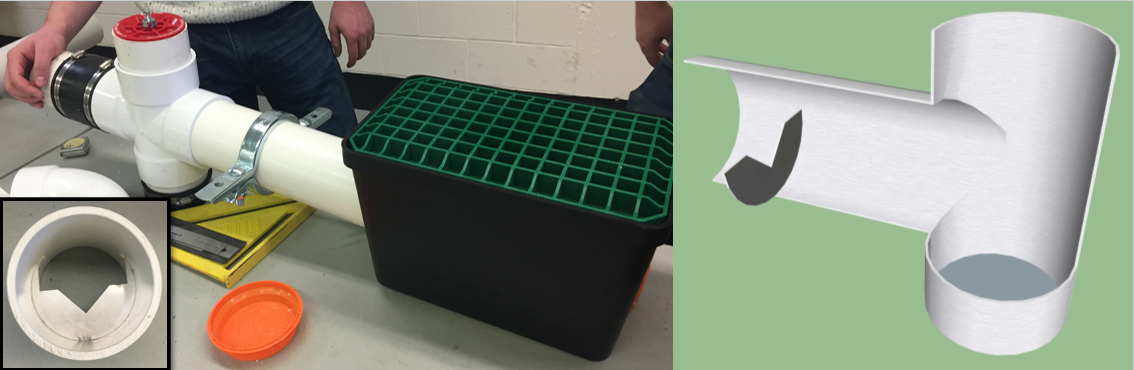
\includegraphics[width=0.8\textwidth]{gfx/chapter-instrumentation/low-flow-setup.png}
	\caption[Low flow measurement setup]{(Left) Low flow measurement setup prototype being constructed in the lab. (Right) Cutaway section of the device outlet.}
	\label{fig:low-flow-setup}
\end{figure}

\begin{figure}[ht!]
	\centering
	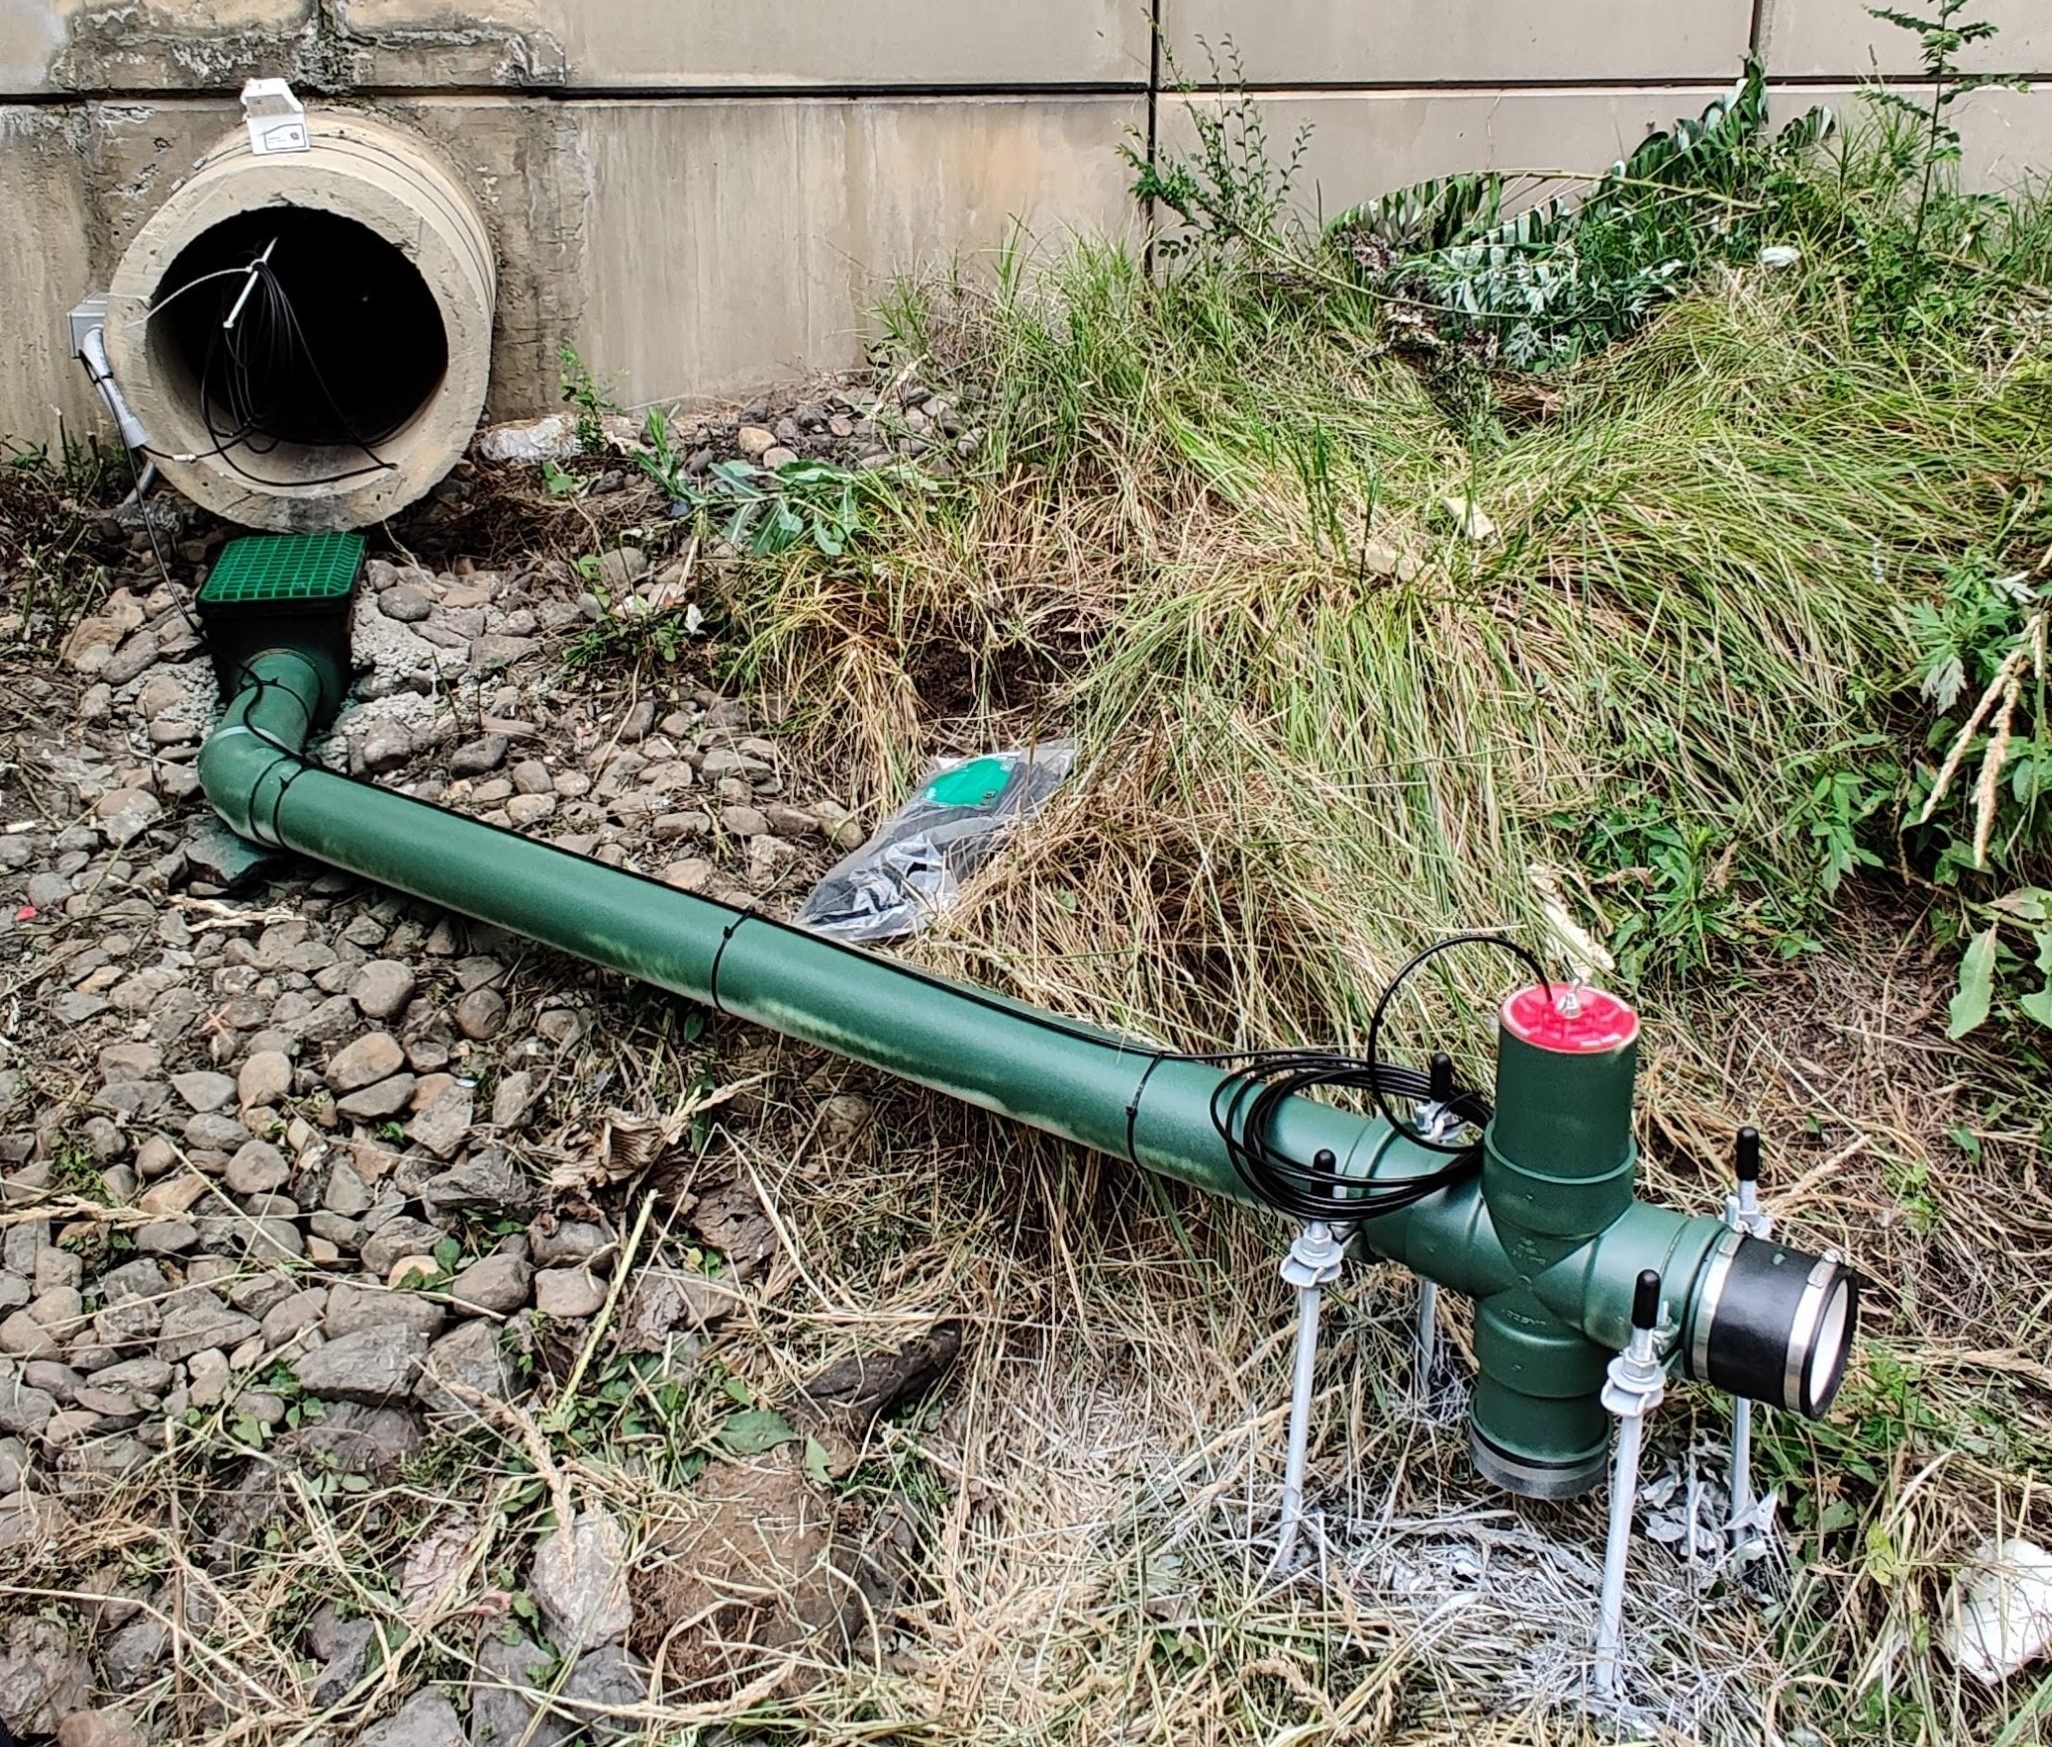
\includegraphics[width=0.6\textwidth]{gfx/chapter-instrumentation/lf-field-install.jpg}
	\caption{Low flow measurement installation.}
	\label{fig:low-flow-install}
\end{figure}

Since installation during summer 2020, the low flow measurement systems at N8, N9, and N10 have captured at least a portion of the flow of each event.
However, several issues remain: the capture efficiency of the inlet (green plastic grate) is lower than anticipated, as a significant percent of flow splashes off and is not captured in the system (Figure \ref{fig:low-flow-splashing}).
Despite this, the inlets show a clear response to rainfall depths as seen in Figure \ref{fig:low-flow-data}.
This data, collected at N9 during a 47mm storm event show a total volume of 3.2$m^{3}$, which equates to just 3.7mm of rainfall over the approximate drainage area of 882$m^{2}$ at N9.
While this could be explained by changes to the drainage area since the LiDAR survey was performed in 2017, bypass due to inlet grate design, or poor capture efficiency at the pour point into the garden, it is evident that the system needs further tuning.

\begin{figure}[ht!]
	\centering
	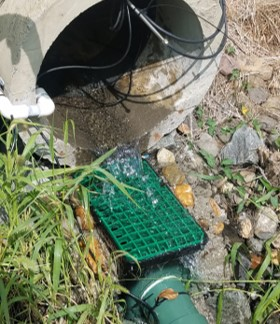
\includegraphics[width=0.5\textwidth]{gfx/chapter-instrumentation/lf-n9-action.jpg}
	\caption{Splashing at N9 low flow installation during September 2020 SRT.}
	\label{fig:low-flow-splashing}
\end{figure}

\begin{figure}[ht!]
	\centering
	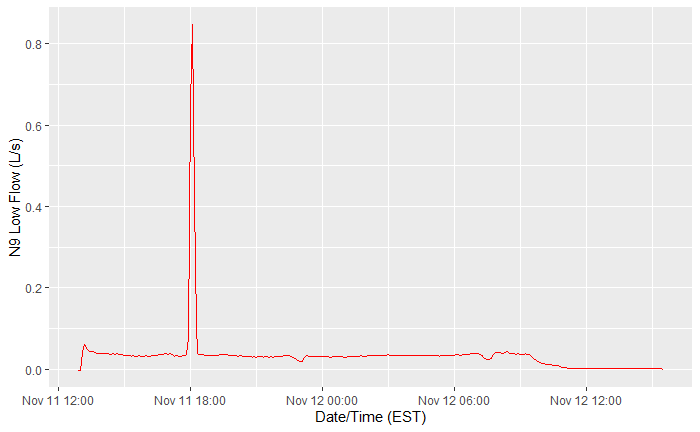
\includegraphics[width=0.8\textwidth]{gfx/chapter-instrumentation/low-flow.png}
	\caption{N9 low flow data for 47mm storm event.}
	\label{fig:low-flow-data}
\end{figure}

\subsection{Future Work}

Investigation into the combination of Blue Siren AV sensor for velocity readings and Massa Ultrasonic depth sensor is ongoing.
Preliminary lab results (Figure \ref{fig:ultrasonic-lab-test-results}) indicate that this system will be sufficiently accurate in combination with the aforementioned low flow system due to their overlap in flow range, shown in orange.

\begin{figure}[h!]
	\centering
	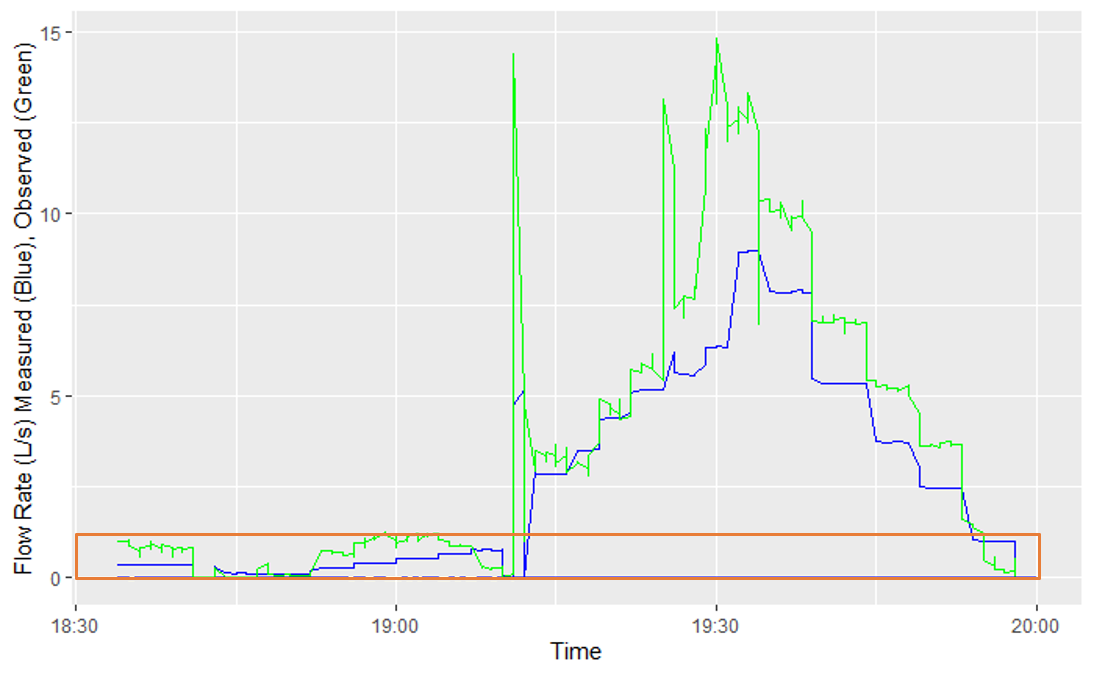
\includegraphics[width=0.8\textwidth]{gfx/chapter-instrumentation/us-flow-test.png}
	\caption{Ultrasonic depth plus Blue Siren velocity preliminary flow comparison.}
	\label{fig:ultrasonic-lab-test-results}
\end{figure}

This system will require further tuning to ensure that the flow rate measurements produced are sufficiently accurate.
The preliminary results show some evidence of hysteresis, when increasing and decreasing flow rates respond differently, but more controlled lab testing is necessary to identify areas for improving this combination of sensors and the CRBasic program that combines the data they produce into a flow rate.
Further testing at more granular flow rates (smaller jumps in flow rate) will help demonstrate whether this system is ready for site implementation.

Finally, due to the variability of analog signal measurement over the long distances in SMP A, conversion to digital measurement will further increase accuracy and reliability.
All lab tests discussed in this chapter have used an analog to digital converter (ADC) between the sensor and data logger as a proof of concept.
The device of choice is a Vegetronix SDI-12 Analog Sensor Translator (Figure \ref{fig:vegetronix}), which supports up to four 0-5V sensors attached and is fully compliant with the SDI-12 protocol.
This inexpensive device will greatly simplify the wiring schematics necessary for using two different sensors (Ultrasonic and AV) for measuring flow at the inlets, as well as shorten the length of wire over which an analog signal must travel.

\begin{figure}[ht!]
	\centering
	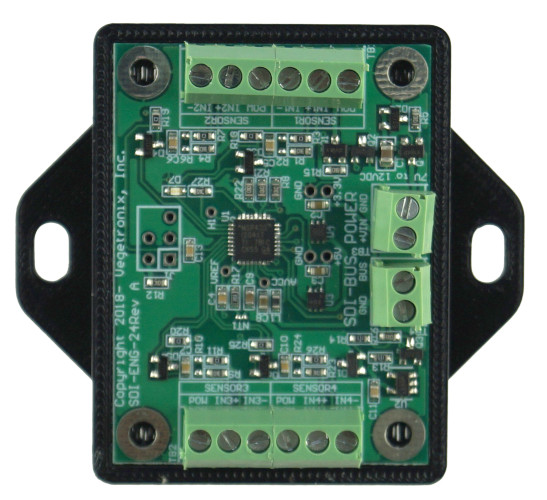
\includegraphics[width=0.2\textwidth]{gfx/chapter-instrumentation/vegetronix-sdi12-converter.jpg}
	\caption{Vegetronix SDI-12 Analog Sensor Translator.}
	\label{fig:vegetronix}
\end{figure}

\section{Conclusions}

Measuring flow in natural, uncontrolled conditions is difficult and requires creativity.
Understanding the intricacies of sensor configurations, communications, randomness of hydraulic characteristics, and opportunities for error can help mitigate invalid data.
Digital communications significantly increase a sensor's ability to report valid data, ensuring that measurements taken in one location are accurately represented and stored by a data logger several hundred feet away.
The increased confidence in data collected will enable future analysis of longer-term trends, so investments and efforts made now in upgrading systems can have lasting benefits for GSI studies across all sites.
Furthermore, significantly less time will be consumed processing the data in quality control procedures leading to more resources available for actual analysis.
% !TEX root = ../main.tex
%
\chapter{Robust Data Storage}
\label{sec:data-storage}

%This chapter will be based on IDM paper and related work (R scripts, IDM formatter, etc...)

\section{Background}

The ability to gain insights from any data set is rooted in good organization of that data.
Large data collections quickly become overwhelming, complex, and site-specific without a comprehensive system for tagging and differentiating data.
None of these qualities are good for developing or deploying easily transferable metrics for evaluating and comparing performance at many GSI sites.
Instead, consistent metadata and uniform data format are two powerful tools for ensuring that data remains accessible and globally applicable in the sense that two data points collected at different sites can be easily understood to measure the same parameter.
The ability to streamline the combination of data from many different sites into a single database with consistent data descriptions has the potential to unlock new insights into performance, long-term and average maintenance needs, and lifespan predictions.
The accessibility of consistently described data reduces the time spent deciphering the meaning, source, and integrity of a dataset.

The need for consistent data definition is not new but has greatly expanded with the decreasing barriers to entry that enable far wider application of monitoring equipment and data collection.
Civil infrastructure has historically taken an approach to building that favors careful planning, site analysis, and construction validation.
The ability to conduct long term monitoring at a wide-spread scale has been lacking due to the difficulty of collecting and analyzing the data necessary at said scale (\cite{DelGrosso2019}).
The ongoing data revolution has the potential to change that, with modern database techniques enabling consistency and accessibility (\cite{Maidment2008,Abdallah2019}).
Several examples of centralized water data repositories exist already including the International Best Management Practices (BMP) database, which provides many observational data points across a range of GSI types and locations (\cite{LIDCenter2004}), the EPA's Storage and Retrieval System (STORET), and USGS' Nation Weather Information System (NWIS).
However, the data in the International BMP Database is largely focused on discrete samples, and the structure of all these systems is not sufficiently standardized to allow for efficient organization of continuously recorded time series data or collaboration with data across different systems.
While discrete data is an important tool in the study of GSI, continuous data is also highly useful and presents a much larger challenge due to the vastly larger scale of the data collected (\cite{Wadzuk2021a}).
A collection of discrete data points may number in the several hundred or perhaps several thousand, while continuous data easily scales to several million values per site over the course of a multi-year study.
A system of standardized "controlled vocabulary" could help alleviate some of these issues (\cite{Maidment2008}), but would require a great effort to sort through many years of historical data, not all of which may be easily identified and traced back to its proper origin.
Therefore, a modern system with the flexibility to accommodate the scope and size of data collected is necessary to enable multi-year, multi-GSI system studies that can fully take advantage of the expansion in data collection (\cite{Wadzuk2021,Meng2017}).

The Consortium of Universities for the Advancement of Hydrologic Studies, Inc (CUAHSI) have created the Observations Data Model (ODM), which aligns better with the needs of continuous monitoring data and has features for publishing data across different research groups (\cite{Horsburgh2008a,Maidment2008}).
However, there are limitations on data categorization because variable and site codes are used to uniquely identify a data point, so sites with multiple identical variables (e.g., two inflow measurements at different locations within a site) are not possible without creating redundant variables.
Additionally, there are data privacy concerns for research sponsors interested in organizing their data without making it publicly available, as required by the included WaterML integrations.
The schema for the ODM provides a robust means for storing time series data, and is flexible enough to be expanded with the additional metadata collected at various VCRWS project sites, including at SMP A on the PennDOT project.
The ODM is the basis for the expanded platform implemented to handle GSI data at VCRWS.

\section{VCRWS Stormwater Infrastructure Data Model (SIDM)}

Recently implemented at VCRWS, the Stormwater Infrastructure Data Model (SIDM), is a modern database approach to disparate data organization using relational tables.
By abstracting the metadata layer of information away, spatial and temporal linkages between data can be stored without repetition of the metadata itself, making storing and accessing data easier and faster.
The SIDM is based on the schema of the ODM and shares many of the same features, but goes a step further by introducing the ability to associate data with specific sample locations within a given site as well as the implementation of protected sharing features.
The web interface was also refreshed to have a modern look and easy navigation.
User permissions and data sharing abilities are facilitated by pages accessible to site administrators.
New metadata definitions for sites, sampling locations, variables, and methods must be created via their respective pages before data related to the new definitions can be imported.
Data import is available to coordinators for each site, allowing the addition of a single data point for discretely sampled data, or uploading a formatted data file for continuous data.

Throughout the development process, the database was designed to align with principles of FAIR (Findable, Accessible, Interoperable, Reusable) data (\cite{Wilkinson2016}). 
The SIDM's updated data format is intended to meet these criteria to enable more robust and sustainable study of data stored within.
The SIDM makes finding data easy through a simple GUI search page with filters for each type of metadata.
The simple, yet effective interface for building queries to search the database allows authorized users the ability to download all data values and associated metadata to a CSV file with the click of a button, making all data easily accessible.
Metadata is stored in data logs, which remain accessible even when their associated data points have been removed.
This has the potential for further analysis with expanded capabilities such as an application programming interface (API) for easy pre-processing and cleaning.
The data model is reusable, as any given combination of space (site, sample location), time, and variable codes uniquely identifies a data point and can be used as a reference for further analysis.
This traceable metadata associated with every data value allows future users to understand what conditions under which the data was collected.
In addition to making data easier to query, this means that auditing work to determine when and how measurement procedures or methods change becomes possible because each new iteration of a data collection method can be tagged with unique metadata.

\subsection{Metadata Standardization and Data Formatting}

The central feature of the SIDM is the relational nature of the metadata abstraction (\cite{Horsburgh2008a}).
Keeping data and metadata separate allows for more efficient storage because there is no duplication of information and for the flexibility to expand the scope of data stored without updating the storage structure.
Each database table uses a primary key column to uniquely identify records.
These primary keys, when used in other related tables to identify pieces of related information, are called foreign keys.
Foreign keys establish the relationship between a data record and its corresponding site, sample location, variable, and other metadata of interest.
Each of these pieces of metadata are stored in their own tables with consistent information describing each record within (Figure \ref{fig:idm-schema}, enlarged in Appendix A).
By linking the related records with the appropriate keys using a unique identifier, duplicate information is not created.
The structure of these relationships allows infinite combinations of spatial and temporal data, while remaining flexible enough to accommodate new or changed data streams without the need for actual structural updates to the data format.

\begin{figure}[ht]
	\centering
	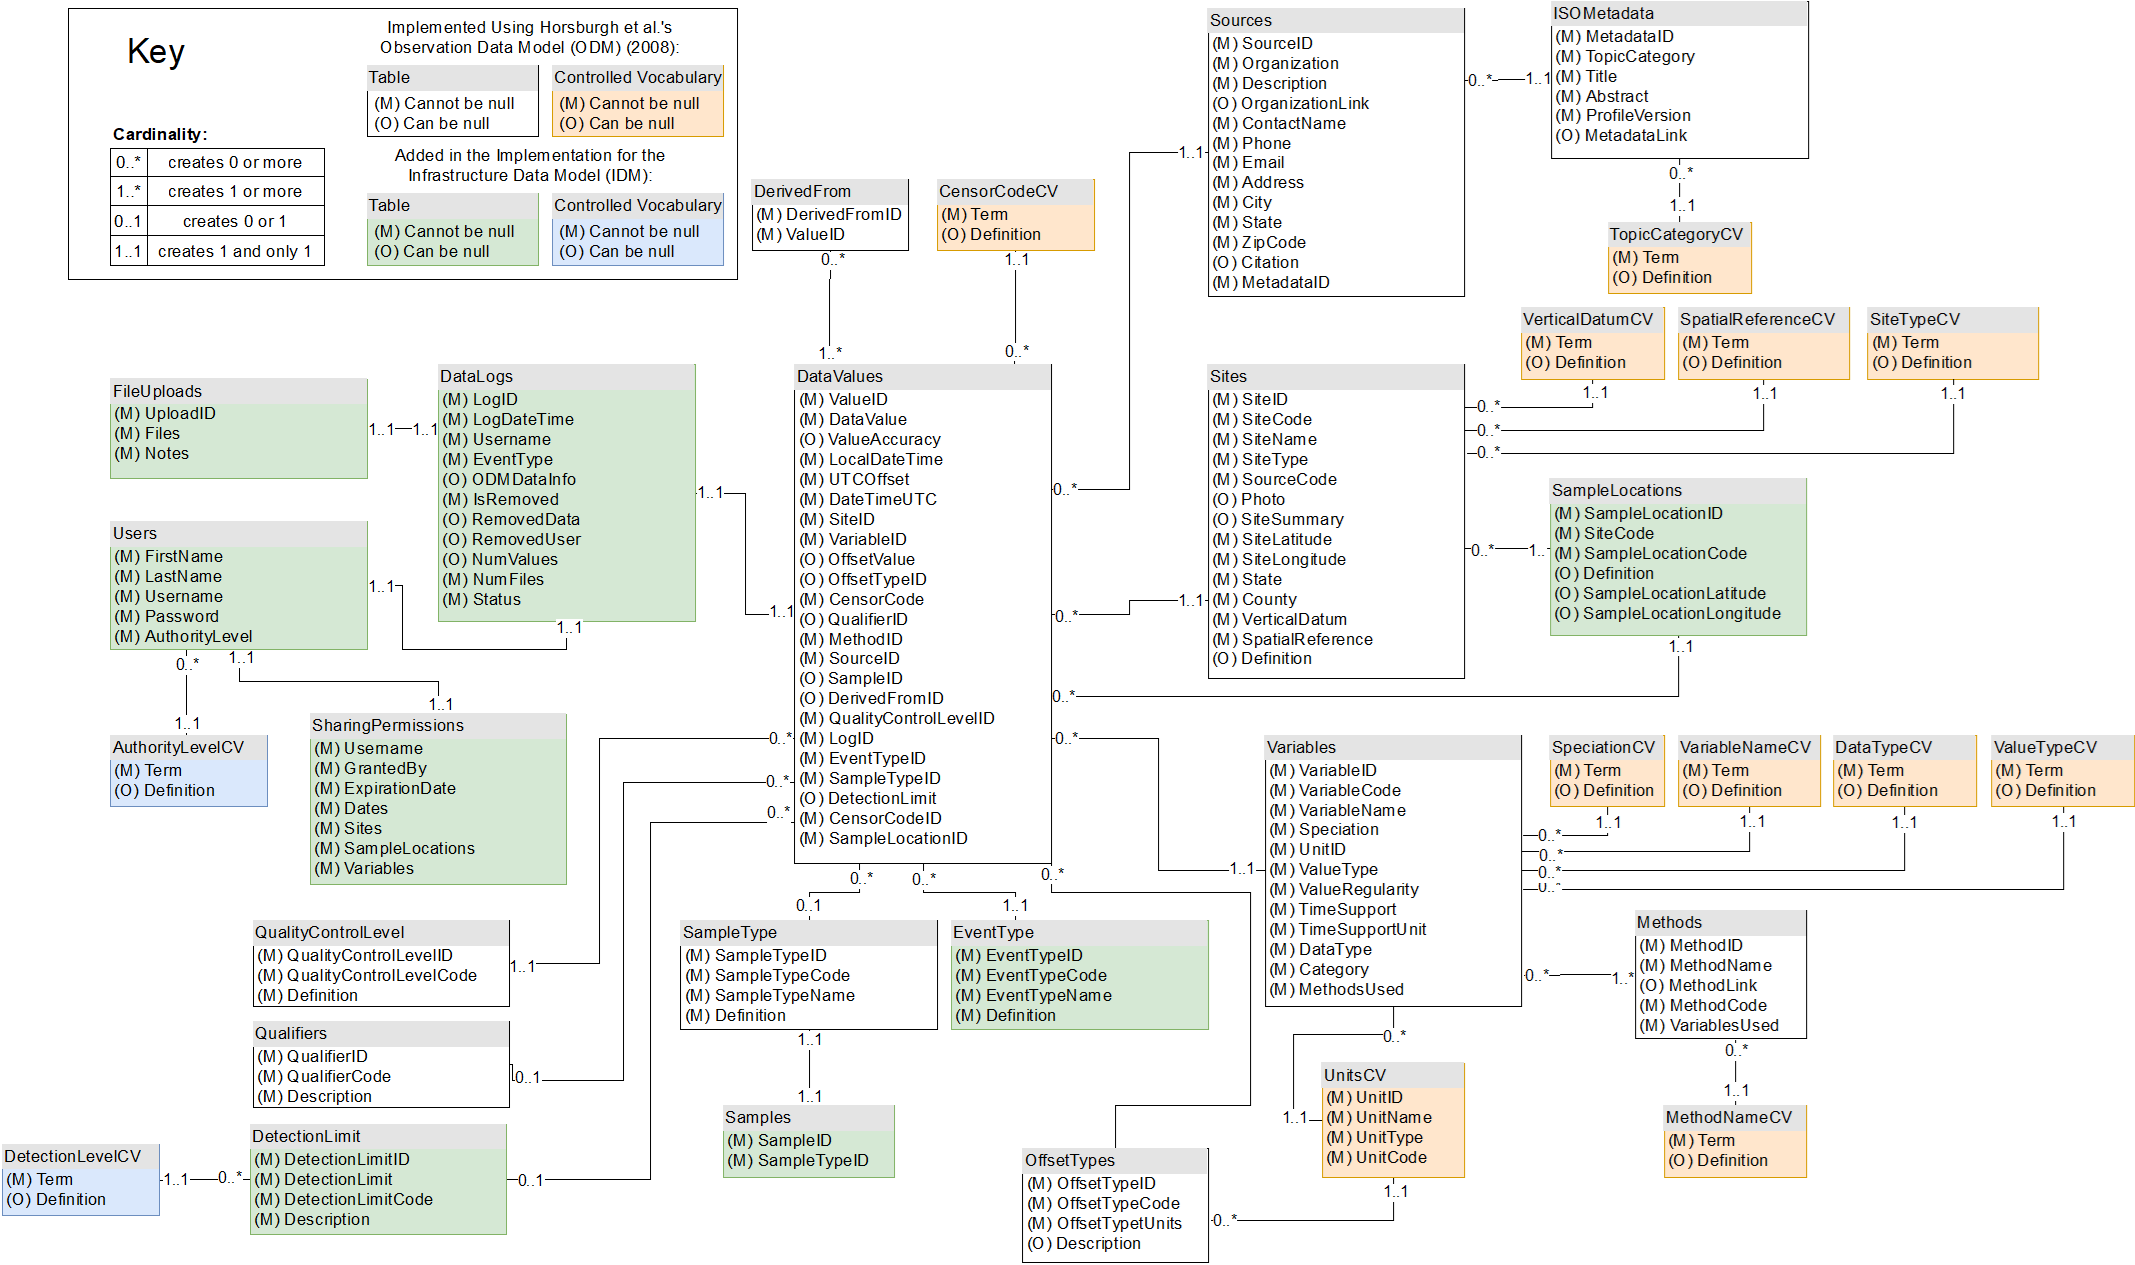
\includegraphics[width=\textwidth]{gfx/chapter-storage/idm_schema.png}
	\caption[SIDM database schema.]{SIDM database schema (Smith et al., submitted).}
	\label{fig:idm-schema}
\end{figure}

Data is collected in a wide format, where each unique variable is stored in its own column and a new row of data is appended to the table for each observational timestamp.
From a storage space perspective, this means that there are $N*M$ rows in the table, where N is the number of observations and M is the number of unique variables.
This is sufficient for storing a dataset related to one and only one site where variables directly correspond to sampling locations.
However, each newly collected variable requires the addition of another column to the table or the creation of a new table, which results in the storage of many missing variables or disjointed data records, respectively.
This approach does not work well when used to combine data from multiple sites, as the column names are the sole form of metadata available to describe variable origins.

An alternative approach, and the one taken by the SIDM, is to abstract the information about a data point's origin (site, sampling location, variable, detection limit, collection method, sample type, and offset information) to separate tables, since this information pertains to many data records.
Storing the identifying metadata only once and referring to it via foreign key constraints in the data records table creates consistency in both metadata format and data record format, which enables faster querying of the data records through the use of covering indices.
Columns in a database containing keys are indexed for faster performance, which requires additional storage space but significantly reduces computational time (\cite{lightstone2010physical}).
A covering index is a composite index made up of a set of all possible columns that could appear in a query, meaning the database only has to consult the index values in order to return results.
This format is referred to as long format, as the number of columns in the data records table is fixed according to the desired metadata for each point and a nearly infinite number of observation rows can be appended without any change to the database schema.
This format only requires that the additional metadata for new variables, sites, or sampling locations be added to the appropriate tables before new data records can be imported.

Transforming continuous monitoring data from wide to long format requires a process called melting, which can be accomplished via packages in nearly any modern general purpose programing language.
During melting, original column names are mapped via a secondary input file containing key-value pairs of corresponding original variable names and the expanded metadata for site code, sample location, and variable name.
This expanded metadata is appended to each data record and then inserted into its own row in the output file, along with the other global inputs available (detection limit, sample type, offset type, event type) since these values are expected to be constant for chunks of continuous monitoring data collected in a single file.
For simplicity of use for those not familiar with programming, a graphical user interface version of this process was created using the R Shiny (\cite{RStudioTeam2020}) platform (Figure \ref{fig:data-formatter}).
The web application expects an input file containing raw data with one `timestamp' column followed by any number of variable columns and a secondary mapping file input with the aforementioned key-value metadata pairs, and specifies sensible global defaults for the other necessary metadata.
Additional date filtering is available if partial file upload is desired.
This is useful in the case where data is appended monthly to site's data file, as that data file can still be processed by the program, with the appropriate filtering in place.
Input data is easily processed at the click of a button, and the output is a file ready for upload directly through the SIDM interface.

\begin{figure}[ht]
	\centering
	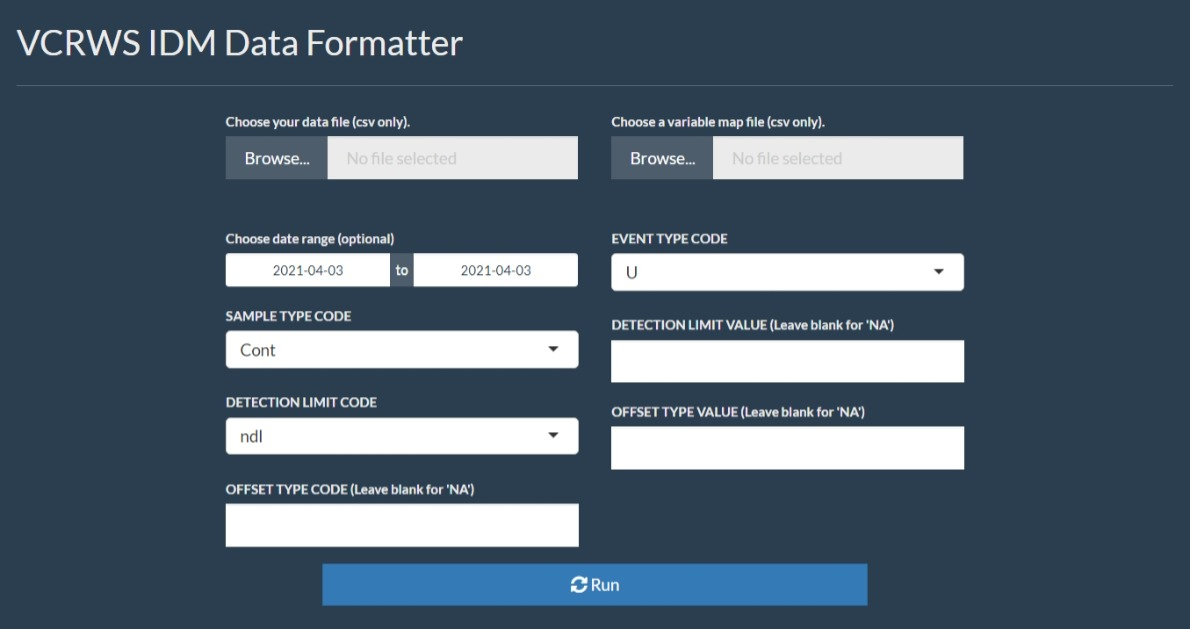
\includegraphics[width=0.8\textwidth]{gfx/chapter-storage/data-formatter.jpeg}
	\caption[R Shiny web app for data formatting.]{R Shiny web app for data formatting (Smith et al., submitted).}
	\label{fig:data-formatter}
\end{figure}




\subsection{Query Performance}

The SIDM web application consists of several pages for uploading data, managing user authentication and authorization, and creating new controlled language for expanding the available metadata.
User accessible pages include a map of all sites showing relative locations with links to a brief site description (Figure \ref{fig:idm-homepage}).

\begin{figure}[ht]
	\centering
	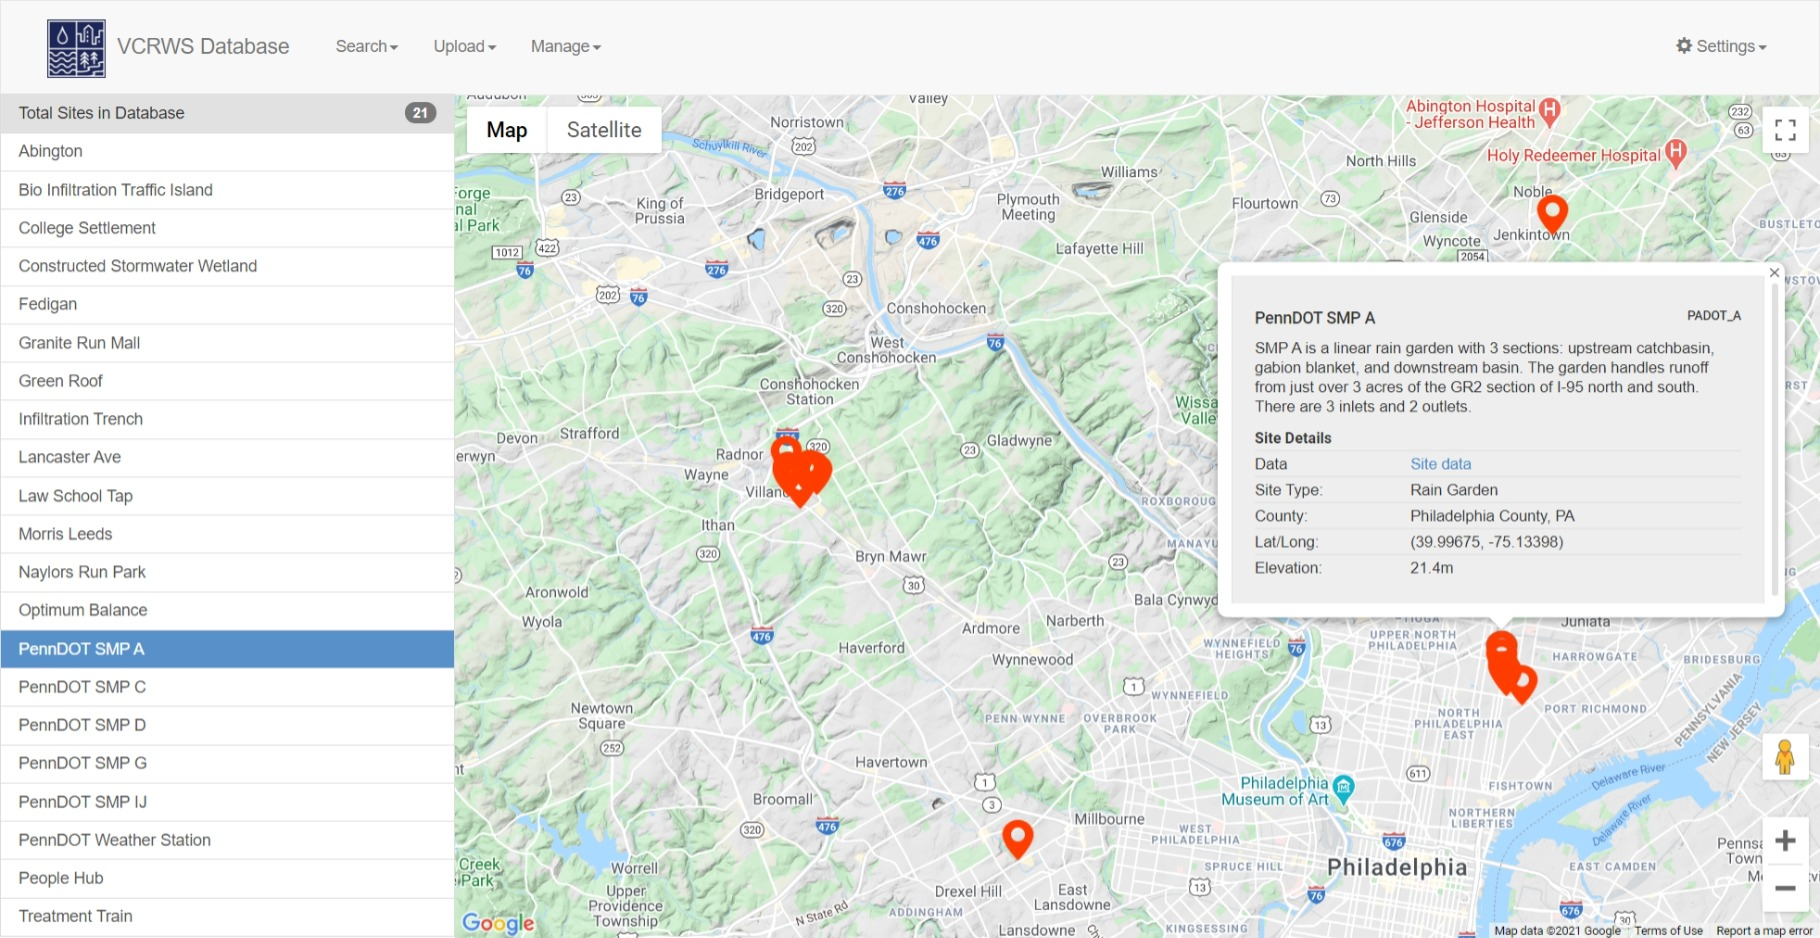
\includegraphics[width=0.8\textwidth]{gfx/chapter-storage/idm-homepage.jpeg}
	\caption{SIDM homepage showing geographical details for SMP A.}
	\label{fig:idm-homepage}
\end{figure}

The query builder page has filter selectors for each metadata parameter that allow a user to select one or more data identifiers, as well as a date range filter.
Once run, the query returns a paginated table of all data requested and gives the option to plot the points in single or multi-axis plots or to download the raw values for analysis in another software package.
The query page is also available to outside users who have access through data sharing links so that project partners can easily access the data.

Query performance is fairly quick given the size of data stored in the SIDM (100M+ data values recorded across all sites as of writing).
Current performance is reflected in \ref{table:query-performance}, and shows a sampling of common queries.
The indexing operations required for this improved performance mean that importing data takes longer than it otherwise would without the need to create indices.
This tradeoff is appropriate because many more query operations than import operations are expected, so the overall computational time is decreased, and compute time is more expensive than the increase in storage space consumed by indices.

\begin{table}[ht!]
\centering
\caption[SIDM query performance benchmarks.]{SIDM query performance benchmarks (Smith et al., submitted).}
	\begin{tabular}{| c | c | c | c | c |}
		\hline
		\multirow{2}{*}{Benchmark} & \multirow{2}{*}{Specifications} & \multicolumn{3}{c}{Performance (seconds to completion)} \vline \\ \cline{3-5}
		& & Query & Export to File & Graph + Statistics \\ \hline
		Small Dataset & \makecell{5 Sample Locations, \\ 6 Variables, \\ 900 Data Points, \\ 57.1KB } & 0.062 & 8.27  & 1.11 \\ \hline
		Large Dataset & \makecell{2 Sample Locations, \\ 2 Variables, \\ 955,762 Data Points, \\ 65.5MB } & 3.62 & 30.51 & 7.73 \\ \hline
	\end{tabular}
	\label{table:query-performance}
\end{table}

\section{Future Work}

\subsection{Streaming Data Ingest}
Currently, the process of extracting, transforming, and loading (ETL) data from the data loggers into the SIDM requires manual input and transfer of files.
Currently, each data logger appends data to a separate file on a remote server, which is accessed monthly to check the data, transform it, and load it into the SIDM.
The process is time consuming, subject to human error, and means that delays of data reaching the SIDM of a month or more are typical.
A better approach would be automatic streaming and loading of the data logger output directly to the SIDM on a close to real-time basis.
An update to the Campbell Scientific CR6 data logger's operating system, which is commonly used in VCRWS monitoring programs, enables the use of the message queueing telemetry transport (MQTT) framework.
MQTT is an internet-of-things (IoT) system that provides a lightweight method for sending and receiving data measurements between smart devices and servers (\cite{MQTT}).
An update to the SIDM could include an API to which the CR6 data loggers can send MQTT messages with up-to-date measurements, greatly enhancing the ability of the platform to automatically ingest new data.
A set of rules for each site and each variable could be used to further enhance this process by evaluating each incoming data point against a set of pre-specified criteria to ensure the integrity of the data or send alerts to users if measurements are out of bounds.
This ingestion system will have the added benefit of requiring more strict linking of physical sensors with their data stores and the rules used to define valid data immediately upon deployment.
Similar data loggers that already have remote connection capabilities could easily have data streaming capabilities enabled via a firmware update.

\subsection{Programmatic Data Retrieval}
The data sharing system of the ODM was removed from the SIDM's feature set to limit the publicity of preliminary data and protect research sponsors who wish to keep their data private.
While there are new methods for sharing specific query results, these still revolve around downloading CSV files containing the data.
There are no methods for programmatically sharing data or querying the database.
Analysis relies on correctly identifying and downloading data prior to beginning analysis, making individual queries difficult to communicate to other researchers.

Modern API design should be used to extend the existing query builder to allow any programming language access to the results of a query through javascript object notation (JSON), a common method for sending large data payloads using the HTTP protocol.
Every common programming language (R, python, MATLAB) used in statistical and modeling efforts supports making HTTP requests and handling JSON response data.
An analysis script could query this API endpoint with the requirements for a dataset of interest and store the server's response before continuing with the necessary calculations.
This would reduce the amount of time required for analysis as a user can directly load data from the server into their analysis program of choice without the need to shuffle data files around, and gathering new data becomes as simple as resending the query request to the server.

\section{Conclusions}

Making data storage FAIR means that data is easily accessible, and analyses performed within a site become easier to transfer to similar sites.
The ability to scale analysis across multiple sites will greatly expand the scope of research that is able to be conducted on larger GSI systems.
This is accomplished through controlled vocabulary for describing data and consistent, yet flexible, formatting of the database schema.
Allowing the addition of new variables at any site or sampling location means that the database can continue to be expanded with new sites and variables without losing the integrity of the historical data already captured.
Furthermore, the increasing accessibility of continuous monitoring through inexpensive IoT devices will mean that future sites are able to be monitored and added to the database easily, greatly expanding the value of consistent formatting and data descriptions.
More specifically, it will be possible to understand how individual systems' performance impacts a larger system.
Finally, VCRWS' SIDM has made significant progress in accomplishing these goals, as VCRWS data stretching back to 2003 across many sites is now contained in a single format.
The SIDM will unlock the potential for expanded collaboration between researchers, better understandings of long-term monitoring results, and more robust analyses of multi-site GSI systems.

% !TEX root = ../main.tex
%
\chapter{Data-Driven Performance Analysis}
\label{sec:data-analysis}

\section{Background}
Green stormwater infrastructure (GSI) systems' performance has historically been difficult to measure due to poor or nonexistent monitoring and inconsistent performance metrics by which to evaluate systems (\cite{Meng2017}).
There are many reasons for this lack of consistency, but much of it stems from the wide range of possible precipitation volumes and intensities producing an equally wide variety of responses by these GSI systems.
Most systems are designed and constructed using specifications drawn up over the last 25 or more years.
The National Pollutant Discharge Elimination System (NPDES) is a common national set of requirements arising from the Clean Water Act (CWA) of 1972 and outlines maximum discharge rates and pollutant loads from certain site types, broken down by activity (industrial, construction, municipal, etc.) (\cite{USEPA2009}).
However, NPDES requirements are typically not verified through a post-construction monitoring plan nor are NPDES criteria tailored to be more suitable for the local environment.

There are few well-defined and agreed upon performance metrics that can be used to quantify a GSI's response to storm events over its lifespan (\cite{Davis2012a}).
Infiltration and evapotranspiration capacity of newly constructed systems is occasionally tested for construction acceptance, but these tests are only performed once at discrete randomly selected points within the system and do not convey a wholistic representation of the GSI's capacity (\cite{Brown2012, DelGrosso2019}).
Longer-term, whole system monitoring and performance analysis using key performance indicators (KPI) that align with and augment existing lab and field tests have the potential to unlock new insights into and understanding of maintenance needs, construction methodology, and design choices by connecting design specifications to real-world performance (\cite{Geberemariam}).

The lack of post-construction monitoring and analysis poses a major roadblock to improving recommendations for the design process that could lead to higher GSI longevity, lower the risk of GSI failure or under-performance, and expedite the creation of uniform standards for GSI comparisons between geographically distinct sites or projects. 
Even when these monitoring requirements are in place, diverse site conditions, geographies, and climates necessitate a standardized framework for quantifying performance and comparing between potentially vastly different sites, such as the International BMP database, SIDM, and others discussed in Chapter \ref{sec:data-storage}.
This chapter outlines proposed key performance indicators (KPI) tailored to an infiltration-type rain garden GSI by looking at historical data for SMP A, located in PennDOT's GR2 section of the I-95 Girard Avenue Interchange Stormwater Project (Figure \ref{fig:site-layout}).
These robust monitoring and analysis techniques will lead to consistent results that can be applied across many sites while ensuring that outside factors do not influence performance measurement results.
The following KPI measures are intended as derivatives of existing, more complicated lab or field tests that are widely accepted, such as infiltration testing, soil texture tests, soil porosity and bulk density tests, to name a few, but are based solely on data collected automatically by a the SMP A sensor network.
This usage of existing data to corroborate more difficult testing procedures' results will allow easier comprehension of the KPIs and wider transferability.
Further, using sensor data will enable cost-effective, sustained monitoring to evaluate performance over time, that more complicated, labor-intensive, and discrete field and laboratory testing programs cannot capture.
A standard approach to analysis will open the door to suggested improvements for designs and further exploration of GSI's importance to more sustainable urban environments.

Recession rate, or the change in depth of water ponded over time, is hypothesized to be a potential key performance indicator (KPI) for GSI because it provides an easy to measure proxy for soil health.
Soil health, in the context of GSI infiltration, is defined as a lack of compaction, clogging, or other infiltration inhibiting issues (\cite{Sokolovskaya2021}).
These properties of soil heavily influence hydraulic conductivity and the shape of a soil-water characteristic curve (SWCC) (Figure \ref{fig:swcc-example}).
Hydraulic conductivity of soil is the property that defines the ability of soil to pull water from the surface and through the soil column, or the ability to reduce pressure differentials within different sections of soil.
The SWCC defines how a given soil responds to varying saturation levels by describing the suction force applied to water in contact with the soil across a range of saturation.
Saturation of soil occurs when all the void space is filled with water and the movement of water through the soil column reverts to a gravity driven system that is largely influenced by soil characteristics.
Saturated soil generally has the lowest hydraulic conductivity, referred to as $K_{sat}$, among the range of all volumetric water content (VWC) values possible for that given soil (\cite{Eyo2020}).
Different soils can have significantly different hydraulic conductivity ranges, and engineered soils with favorable properties (higher saturated hydraulic conductivity) are generally specified for GSI design where infiltration is a desirable treatment method.
Infiltration capacity is a function of soil saturation level, and a completely saturated soil will have the lowest infiltration rate, much like it has the lowest hydraulic conductivity.
Once fully saturated, infiltration continues at a fixed rate, which is a proxy for saturated hydraulic conductivity.
The saturated infiltration rate is hypothesized to be a KPI for system health as it indicates capacity to store water below the soil's surface.
This infiltration rate continues even after ponding has ended, as the zone of fully saturated soil extends above the water table level where full saturation is essentially permanent.
Significant, long-term water table mounding has not been found to occur as a direct result of infiltrating GSI practices (\cite{Tu2019, Machusick2011}), meaning that infiltrating water generally recedes until it reaches the normal water table level.
Therefore, infiltration should be expected to continue downward at a constant rate resulting in the steady recession of the saturated zone along a `drying front' similar to the `wetting front' seen at the beginning of saturation.
The following sections discuss the data collected at SMP A used to support these hypotheses and show that the recession rate and soil drying rate can be used as proxies for soil health and extended to overall GSI performance.

\begin{figure}[ht]
	\centering
	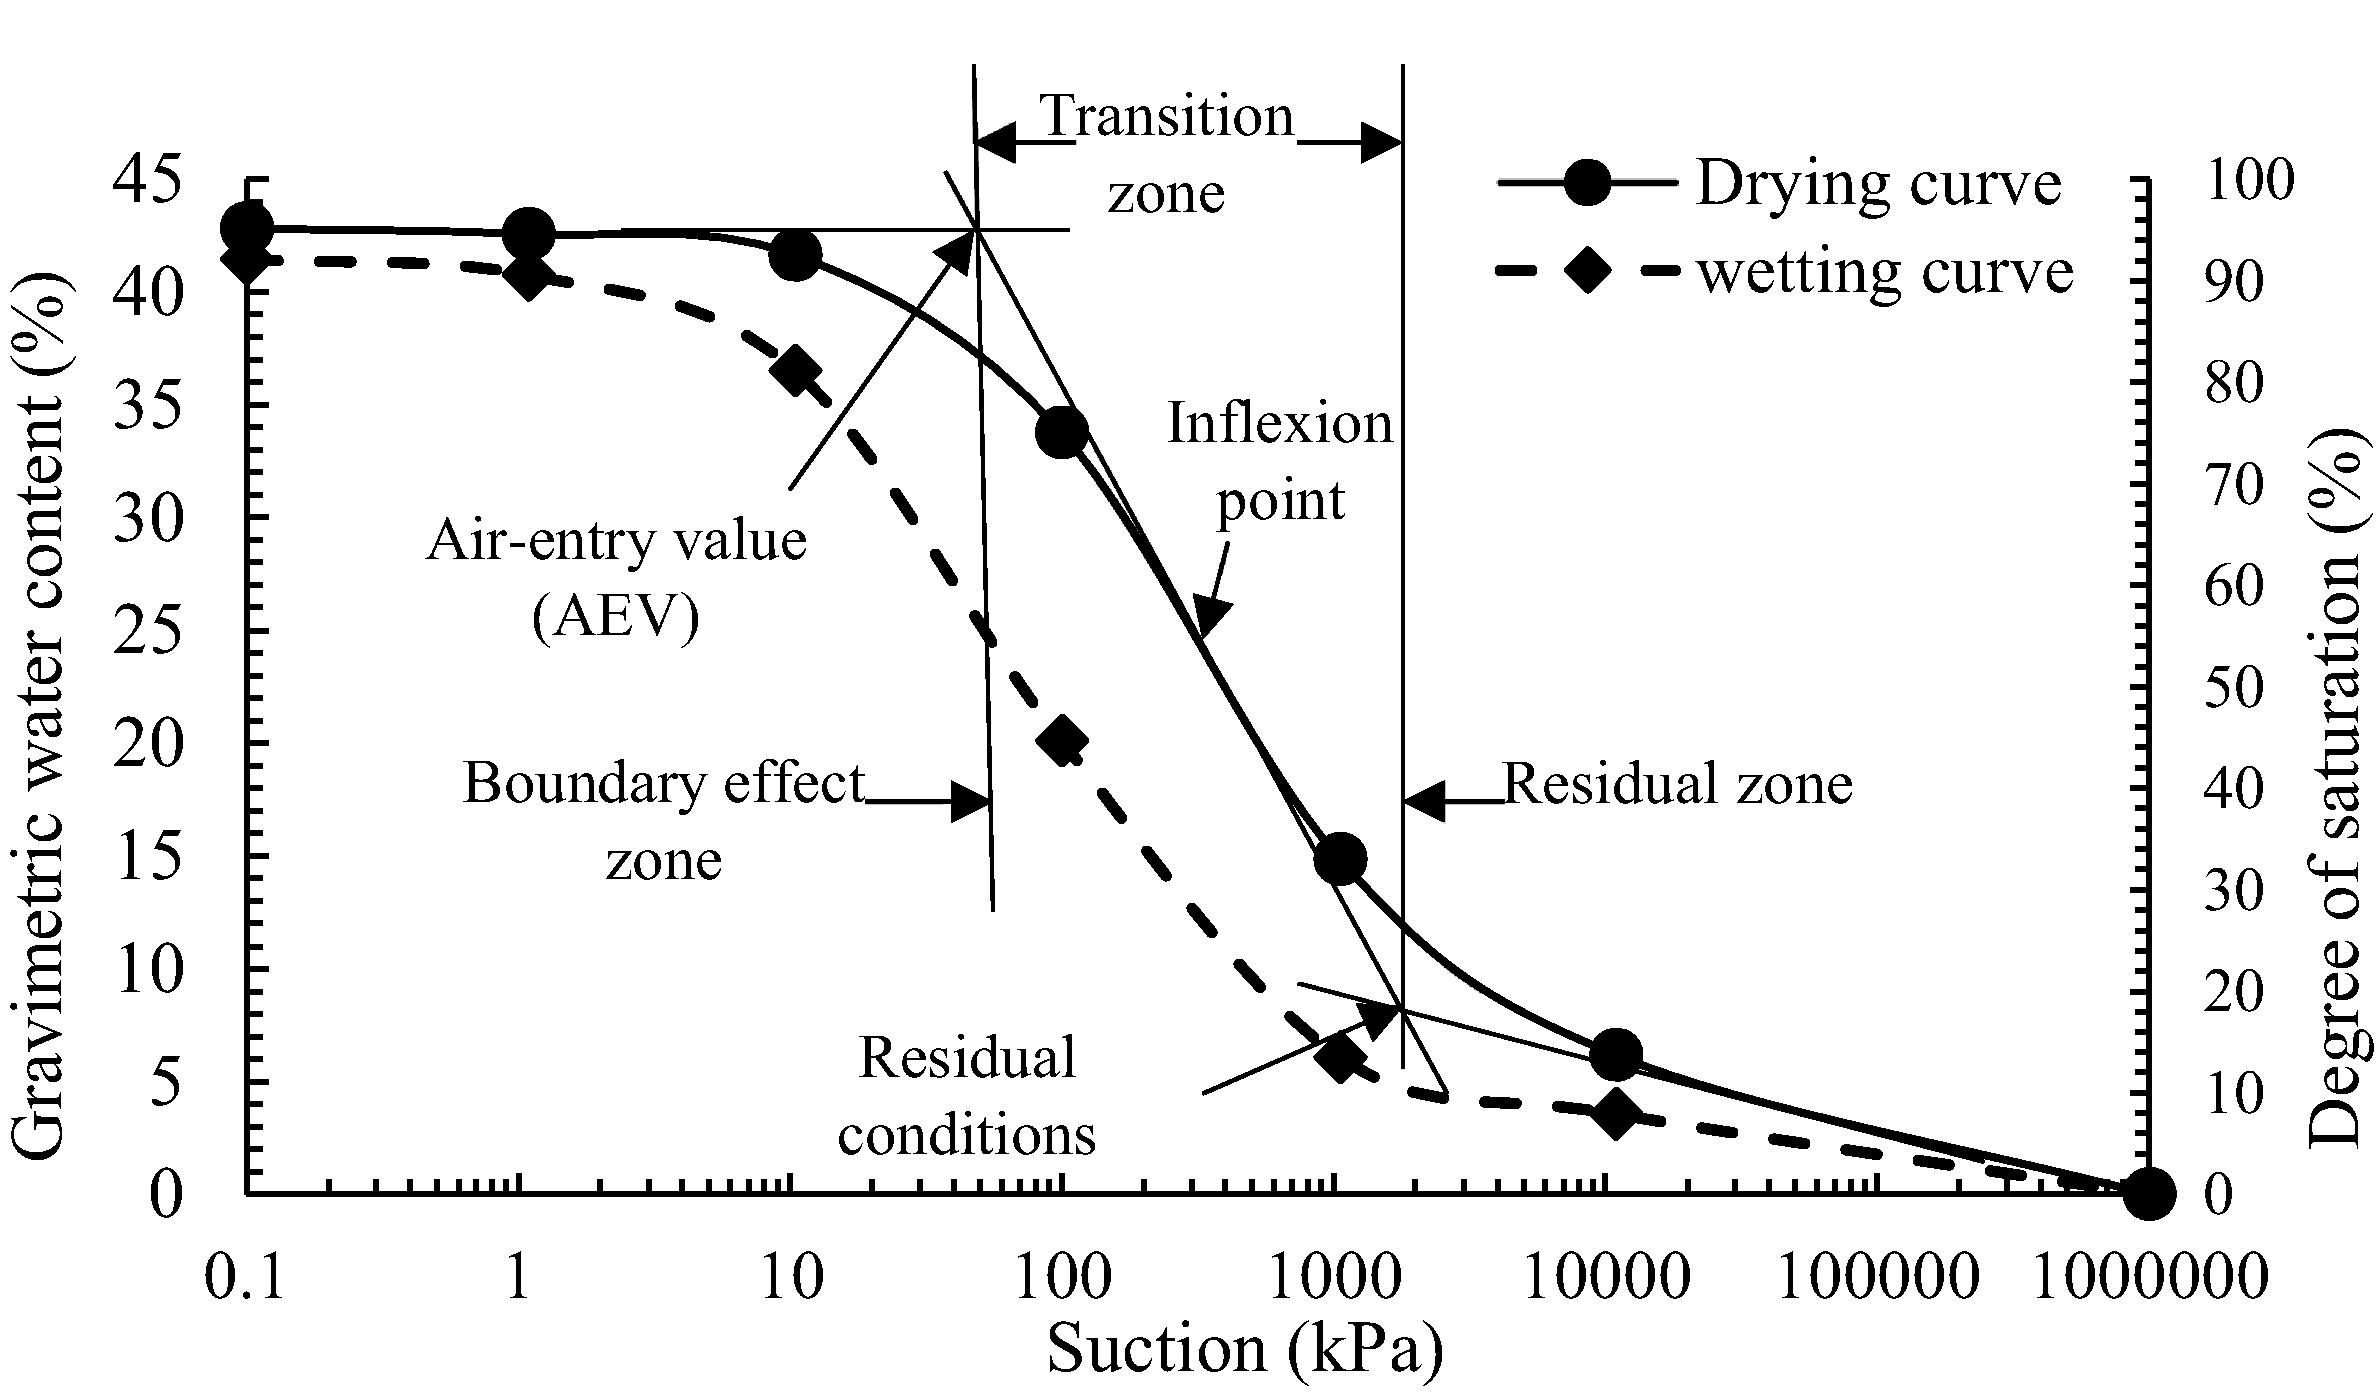
\includegraphics[width=0.8\textwidth]{gfx/chapter-data-analysis/swcc.jpg}
	\caption[Example SWCC.]{Example SWCC (\cite{Eyo2020}).}
	\label{fig:swcc-example}
\end{figure}

\section{Data and Modeling}
Data collected was 5 minute averages of 1 minute records (values were measured every minute and stored every 5 minutes as the average of the previous 5 values) over the course of the 3 year study (May 2017 - November 2020).
This data resolution captures enough detail without producing an overwhelming number of data records.
To better synthesize the data collected, summary statistics for predefined hydrological events are generated based on either a total amount of rainfall followed by a minimum dry time (typically 6 hours), or based on characteristics of other variables of interest, namely ponding and soil moisture values.

\subsection{Rainfall Events}
Using clearly defined rules to identify events is the first step to generating meaningful summary statistics that are applicable across time and space, and useful for comparing GSI with dissimilar properties.
In a GSI context, events are storms that result in a measurable quantity of precipitation.
Small events typically do not have a pronounced impact on GSI, but the effectiveness of GSI systems is typically greater for smaller or less intense storm events (\cite{Liu2020}).
However, these smaller events make up the bulk of storm events observed at SMP A and by others (\cite{Albright2018}), with 95\%\ of observed total rainfall less than 42mm (Figure \ref{fig:event-total-rainfall}).
For this analysis, a `standard,' or `normal' storm event begins when rainfall is first recorded and continues until 6 hours after the last observed rainfall, as studies have shown storms separated by 6 or more hours to be meteorologically separate events (\cite{Wadzuk2017}).
This means the minimum event duration is 6 hours, and any periods without rainfall of less than 6 hours are continuations of the same storm event.
This definition is used as the standard both for generating storm summary data in monthly reports to PennDOT and for all analyses henceforth that do not directly involve soil moisture observations.
During the period of interest, there were 414 observed standard events with a mean duration of 12.2 hours, a median of 9.5 hours, and a standard deviation of 7.5 hours. The data are highly right-skewed, with a maximum of 52.2 hours, and appear to follow a roughly chi-square distribution (Figure \ref{fig:event-duration-histogram}).

\begin{figure}[ht]
	\centering
	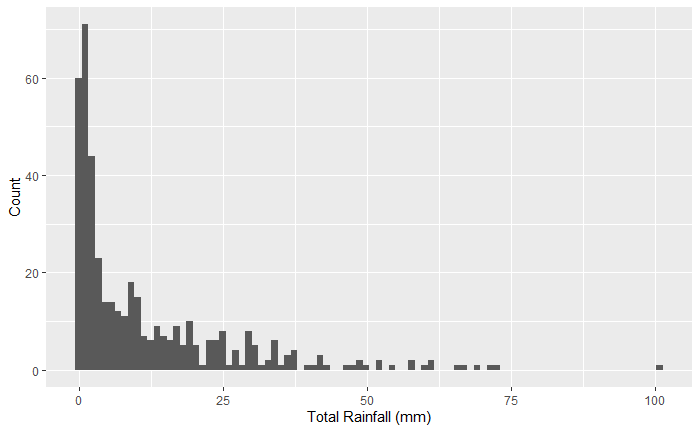
\includegraphics[width=\textwidth]{gfx/chapter-data-analysis/hist_rainfall_depth.png}
	\caption{Distribution of event total rainfall depths.}
	\label{fig:event-total-rainfall}
\end{figure}

\begin{figure}[ht]
	\centering
	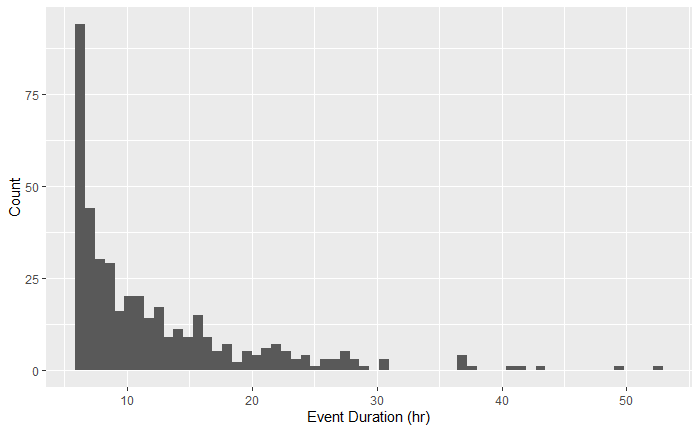
\includegraphics[width=\textwidth]{gfx/chapter-data-analysis/hist_duration.png}
	\caption{Distribution of event lengths.}
	\label{fig:event-duration-histogram}
\end{figure}

Events are distributed throughout a Gregorian 365-day year approximately uniformly, as seen in Figure \ref{fig:event-date-histogram}, although there are some notable event clusters in both late spring (around ordinal day 150), and during hurricane season (after ordinal day 200).
There are notably fewer events during the winter months, but this is likely due to the instrumentation's lack of sensitivity to snowfall.
Snowfall events are also less taxing on GSI systems in general, although snowmelt events may have similar characteristics to a rainfall event but have not been studied.

\begin{figure}[ht]
	\centering
	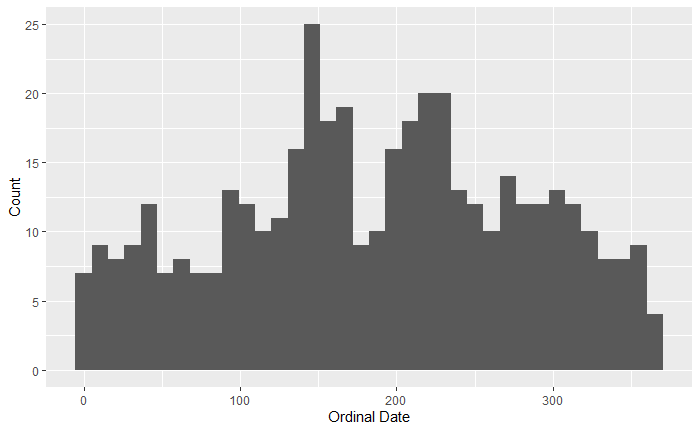
\includegraphics[width=\textwidth]{gfx/chapter-data-analysis/hist_ordinal_date_event.png}
	\caption{Distribution of event ordinal dates.}
	\label{fig:event-date-histogram}
\end{figure}

\subsection{Soil Moisture Events}
Events involving soil moisture require a modified approach to event definition due to the prolonged nature of soil moisture's response to storm events.
Soil moisture, and by extension ponded water atop saturated soils, take longer than 6 hours to recover after storms of interest.
Studies have shown that the recovery period for soils is 72-96 hours (\cite{Davis2009,Wadzuk2017}).
To define events for these analyses, both rainfall and soil moisture levels are considered.
As before, an event begins with the first observed rainfall.
However, the end of the event is defined by a user-defined minimum event time (6 hour default) as well as a threshold ponding level or soil moisture level (either may be used, depending on the type of analysis being performed).
A simple moving average of the number of steps comprising the minimum event duration (in other words, the data interval - 5 minutes - divided into the minimum event time of interest) provides a window into the past or the future at a given time step, and can be used to define an event as follows:
\begin{equation}
	\begin{aligned}
		\centering
		Event = & \{ A = [ moving\_average(rainfall, Q / P) > 0 ], \\
				& B = [ moving\_average(rainfall, Q / P) == 0 \\
				& \cap moving\_average(K, Q / P) < R ] \}
	\end{aligned}
	\label{eq:alt-event-definition}
\end{equation}
where A is an indicator for the beginning of an event, B is an indicator for the end of an event, Q is the minimum event duration, P is the observation interval, R is a threshold value, and K is the variable of interest.
Timestamps falling between successive A and B values are assigned a unique, random string of eight characters generated from the first timestamp in the series.
The distribution of these specialized events is similar to that of the standard events above, although there are fewer (214) of them due to the increased length of events capturing a greater share of rainfall per event.

\section{Key Performance Indicator Definitions}

\subsection{Recession Rate}

Calculating a water level differential across consecutive data records can be used to determine periods of increasing or decreasing volume in the ponded storage.
Recession of the pond is indicated by a negative change in level, although no rainfall or inflow can happen simultaneously to ensure that change in level is solely due to outflow from the system (i.e., infiltration or overflow).
Additionally, if the recession rate due to only infiltration is desired, the water level must be below the overflow point of any outlet structures.
The magnitude of recession is directly correlated to infiltration rate, which is governed by the type and health of the GSI soils (\cite{Gregory2006, Horton1994}).
Larger recession rates indicate a faster drawdown of the water level, while smaller values could be due to prolonged saturation conditions or under-performance due to compaction or clogging of soil pores.
Comparing average recession rates calculated over the duration of a storm to other simultaneously recorded atmospheric (temperature, relative humidity, barometric pressure) and GSI state (current pond level) data shows the relationships that have the most significant impact on GSI performance.
Changes in the recession rate over the period of a storm or over long periods of time (e.g., seasonal, annual, etc.) indicate changes in the soil health (\cite{Jenkins2010,Zukowski2016}).

The relationships between recession and atmospheric variables or GSI state are complicated by several factors, namely the timing and size of an event, the pre-event geomorphology and hydrologic state of the GSI, and their collective interaction.
The timing and size of a storm event, which can be best described by a combination of time of year, hyetograph, and the length of time since the previous storm event, are important because these play the largest role in determining the GSI pre-storm state's response to specific storm conditions.
A GSI system will respond differently at different times of the year to two events with identical hyetographs, while the same GSI with identical starting conditions will respond differently to two different hyetographs (\cite{Braga2007,Joshi2019}).
Varying any single variable used to describe an event changes the GSI system's initial response to that event.

The variability of the pre-event state of the GSI necessitates an adaptable baseline to use in evaluating performance.
Performance cannot simply be stated as the change from pre-event conditions because this would make comparisons between dissimilar pre-event states unnecessarily complex.
For example, a storm taking place during early spring in the Philadelphia, PA region could have a wide range of pre-storm soil moisture, air and water temperatures, or plant growth conditions, to name a few, all of which will impact how the system responds at the beginning of a storm.
Additionally, the fact that suction head is highest when the soil is dry (\cite{Eyo2020}, Figure \ref{fig:swcc-example}), means that infiltration loss is greatest at the beginning of an event, no matter the specific initial conditions, because that is when the soil is driest.
This inverse relationship indicates that the most consistent method of comparison will be when the system reaches equilibrium and is treating water at a constant rate.
For recession rates, this means looking at the trailing end of a storm, when inflow has ceased, ponding level has reached its peak, and the soil has reached saturation.
Examining the end of a storm removes the influence of a specific storm event's timing characteristics and focuses the performance evaluation on how the system reduces ponded volume and recovers from saturation.
Full infiltration of ponded water is required within 72 hours in Philadelphia.
Observations show that the majority of storms have complete infiltration of the ponded water within 6 hours post-rainfall.

\subsection{Infiltration Drying Rate}
The recession of water within the soil column also reflects the soil health of the site.
Using soil moisture probes at 10, 35, and 60 cm allows the calculation of an average rate of the descent of saturation conditions, or `drying front', as the soil capacity recovers.
This subsurface drying rate should remain consistent between events of different sizes (\cite{Wadzuk2017}), provided the soils reach saturation prior to the end of measurable ponding.
Soil moisture values during a storm event typically produce a curve like that in Figure \ref{fig:typ-soil-moisture}.
The soil moisture curve tends to respond with a sharp upward jump, 5-20 minutes in length, at the beginning of the storm event's inflow when the wetting front passes each sensor and soil approaches full saturation.
This increase in saturation coincides with a sharp drop in suction head, as the soil's ability to pull water in quickly is greatly reduced once saturated.
The soil moisture curve has been characterized with a series of seven points in work completed by Matina Shakya, a Ph.D. Candidate working on soil moisture measurements for VCRWS/PennDOT.
The beginning and end of this increase in soil moisture at the inflow onset are identified as points A and B, respectively.
Point A is typically below 0.40, or 40\% volumetric water content (VWC), while points B and C are typically between 0.45 and 0.50, or 45-50\% VWC.
Soil moisture levels remain at saturation conditions for the duration of ponding, due to continuous infiltration.
The reduction in volume from the system due to evaporation, evapotranspiration, or any other means is assumed to be negligible compared to infiltration during a storm and in the hours immediately after.
When ponding has ended, infiltration continues as the saturated zone recedes down into the soil profile (Figure \ref{fig:drying-rate-sketch}).
The trailing limb of the saturation curve can be identified by two additional points, C and D (Figure \ref{fig:typ-soil-moisture}), identified as the drop off point and inflection point of the soil moisture curve, respectively.
In Figure \ref{fig:drying-rate-sketch}, the difference in time between steps 2 and 3 at each sensor depth (10, 35, 60cm) is the subject of interest.

\begin{figure}[ht]
	\centering
	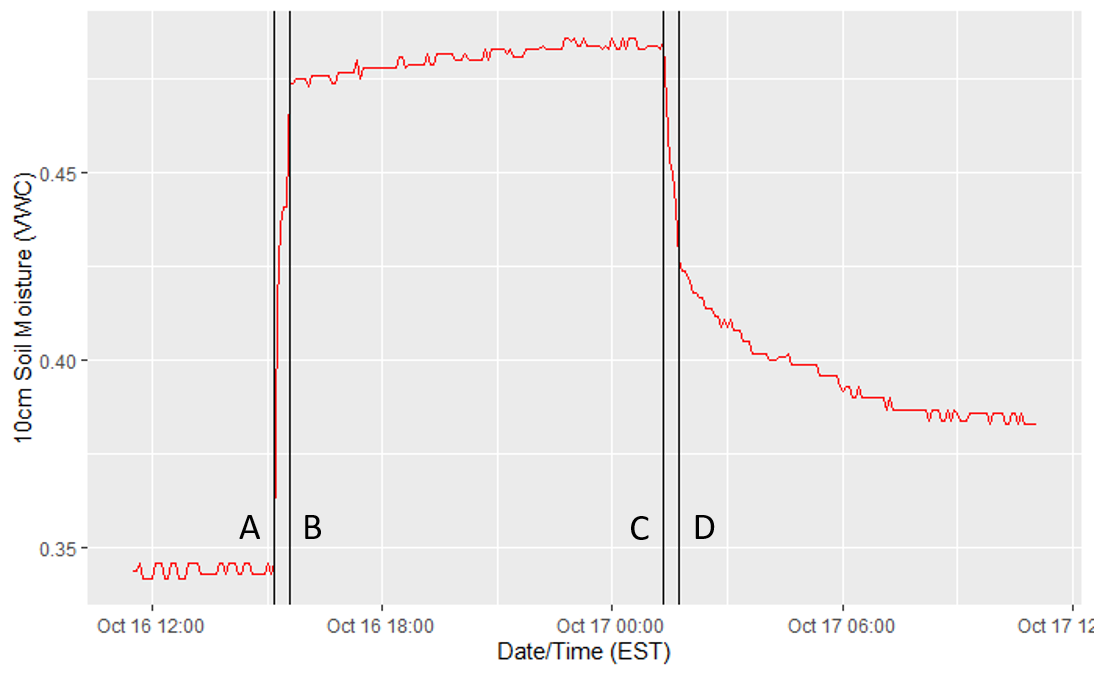
\includegraphics[width=\textwidth]{gfx/chapter-data-analysis/typ_soil_moisture.png}
	\caption[Typical soil moisture curve.]{Typical soil moisture curve. Vertical black lines denote points A, B, C, and D from left to right, respectively.}
	\label{fig:typ-soil-moisture}
\end{figure}


\begin{figure}[ht]
	\centering
	
\includegraphics[width=\textwidth]{gfx/chapter-data-analysis/drying_rate_sketch.png}
	\caption[Illustration of infiltration drying rate.]{Illustration of infiltration drying rate showing 1. ponded water, 2. end of ponding, 3. top-most soil returns to field capacity, 4. saturation zone reaches equilibrium with water table.}
	\label{fig:drying-rate-sketch}
\end{figure}

The calculation of this metric is slightly more complicated than raw recession rate of the ponded water presented earlier.
The inflection points A, B, C, and D are calculated as the four primary peaks in the absolute value of the first differential of the soil moisture data:

\begin{equation}
	\centering
	Inflection Point\{A,B,C,D\} = local max(|\theta_{i} - \theta_{i-1}|)_{j}
	\label{eq:soil-moisture-inflection}
\end{equation}

where i = {1,2...n} for n soil moisture observations ($\theta$) in a given storm and where j = {1,2,3,4} corresponding to {A,B,C,D}.
These points are easily calculated using the `findpeaks' function from the R package `pracma' (\verb+pracma::findpeaks(...)+).
The function takes a vector of data, the absolute value of the differential soil moisture data applicable to one storm event in this case and returns the ordered indices of the requested number of local maximums (four in this case).
Depending on the specific values of soil moisture seen during an event, the four indices may be returned in any order, largely based on the magnitude of difference between any two given points, so the resulting points are sorted and assigned to A through D respectively.
However, due to the highly variable pre-event state of the GSI, storm events that begin with saturated VWC values (>0.44 VWC) often misidentify some or all of these points, so these events have been disregarded in the context of this analysis.

\section{Results and Discussion}

\subsection{Recession Rate}

\subsubsection{Temperature Dependence}
The weather station at SMP A records air temperature, and each pressure transducer (PT) records the temperature of surrounding water.
The two types of temperature are highly correlated (Pearson correlation = 0.981).
This analysis only considers water temperature since the water is in direct contact with the soil and displays some variance of viscosity at different temperatures.
Testing for variations in recession rate across the range of observed water temperatures shows a linear relationship (Figure \ref{fig:temp-vs-recession-by-storm}), as evidenced by the high correlation coefficient of 0.735 and $R^2$ of 0.54.

\begin{figure}[ht]
	\centering
	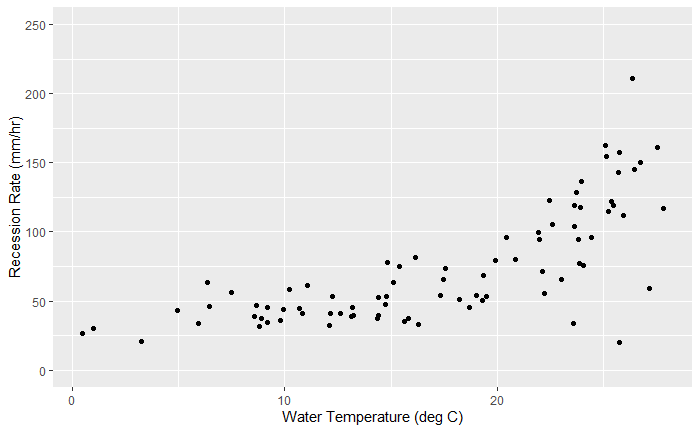
\includegraphics[width=\textwidth]{gfx/chapter-data-analysis/temperature_vs_recession_rate_by_storm.png}
	\caption{Average water temperature vs recession rate for SMP A storm event.}
	\label{fig:temp-vs-recession-by-storm}
\end{figure}

The relationship between recession rate and ponded water temperature becomes more apparent when temperature is separated into similar temperature range bins (Figure \ref{fig:temp-vs-recession-binned}).
Five bins were chosen to ensure the number of events per bin was at least 10 for most bins.
The trend of higher observed recession rates at higher temperatures is clear.
The lowest bin ((-0.05,5.83]) has only seven events but follows an identical trend to the upper four bins in magnitude of mean and quartiles (indicated by upper and lower vertical lines).
This trend aligns with several physical and hydrologic models, namely that warmer water is less viscous and flows easier, especially through the soil (\cite{Emerson2008}).
This finding means that GSI performance can be expected to increase during warmer months, both due to increased infiltration capacity and increased water uptake and evapotranspiration by the plant mass (\cite{Bartens2008}).
Furthermore, it has been shown that soils that have experienced multiple freeze-thaw cycles have higher values of saturated hydraulic conductivity due to the formation of internal ice crystal structures within frozen soils, which can expand pore space and increase the "development of macroscopic cracks and microscopic voids" (\cite{Asare1999}).
Therefore, soils that experience freezing conditions followed by warm conditions, as is typical in a climate with a distinct harsh winter season, can expect to see a natural "loosening" of the soil via the creation of these additional void spaces.
This increase in void spaces has the potential to cause preferential flow paths through the soil, which will lead to increased infiltration rates up to the frost line.

\begin{figure}[ht]
	\centering
	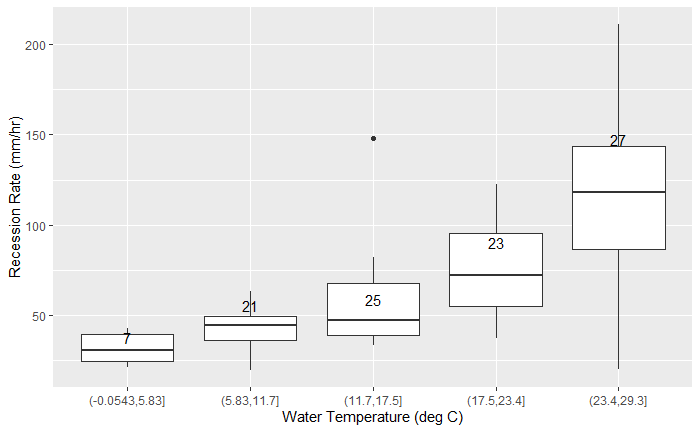
\includegraphics[width=\textwidth]{gfx/chapter-data-analysis/temperature_vs_recession_rate_binned.png}
	\caption[Average water temperature vs recession rate.]{Average water temperature vs recession rate, separated into bins, with the number of storm events per bin indicated.}
	\label{fig:temp-vs-recession-binned}
\end{figure}

\subsubsection{Insignificant Relationships}
Both relative humidity (RH) and barometric pressure, recorded in a similar fashion to air temperature at SMP A, showed no significant relationship with recession rate, with correlation coefficients of 0.148 and 0.25 and $R^2$ values of 0.022 and 0.064 respectively.
Comparing the average recession rate to RH bins and pressure bins shows no correlation between different values for these variables as compared to the average recession rate (Figure \ref{fig:recession-rh-bin} and \ref{fig:recession-pressure-bin}).

\begin{figure}[ht]
	\centering
	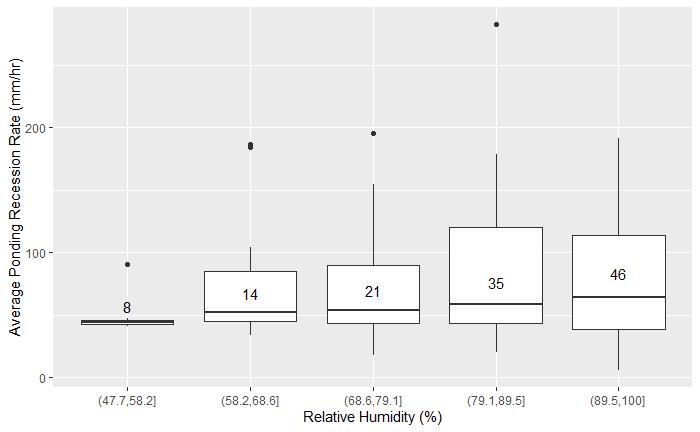
\includegraphics[width=\textwidth]{gfx/chapter-data-analysis/rh_vs_recession_rate_binned.png}
	\caption{Average Relative Humidity vs Recession Rate.}
	\label{fig:recession-rh-bin}
\end{figure}

\begin{figure}[ht]
	\centering
	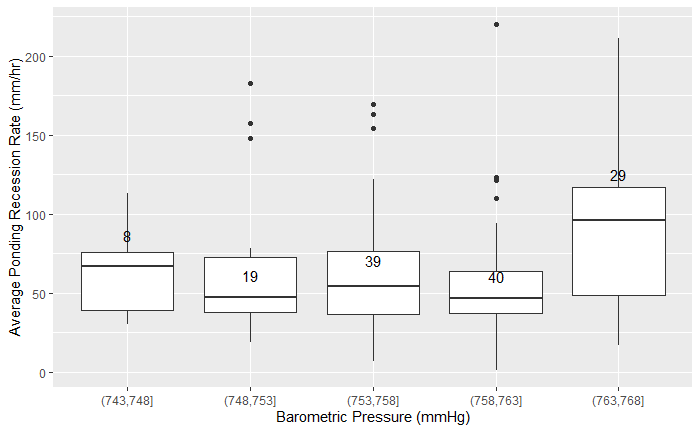
\includegraphics[width=\textwidth]{gfx/chapter-data-analysis/pressure_vs_recession_rate_binned.png}
	\caption{Average Barometric Pressure vs Recession Rate.}
	\label{fig:recession-pressure-bin}
\end{figure}

From these observations, GSI performance is not dependent on barometric pressure or relative humidity, which largely only impact the soil-air interface.
The lack of relationship between the atmosphere and sub-surface infiltration mechanics is expected, since the soil contains enough mass to prevent significant influence from the relatively fast-changing atmosphere.

The level of ponded water collected in the rain garden similarly has no significant effect on the rate of recession, with a correlation of -0.2 and $R^2$ of 0.043.
This runs contrary to expectations that greater head pressure at the soil-ponding interface would lead to higher recession rates.
The rate of recession is consistent across nearly the entire ponding depth range (Figure \ref{fig:recession-ponding-depth-bin}).
\begin{figure}[ht]
	\centering
	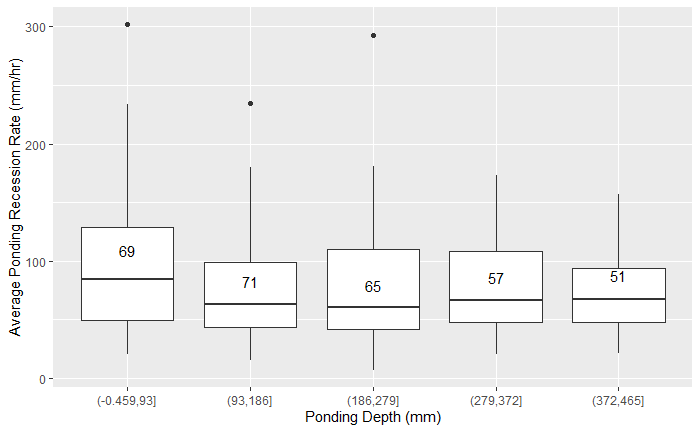
\includegraphics[width=\textwidth]{gfx/chapter-data-analysis/pond_depth_vs_recession_rate_by_storm.png}
	\caption{Average Ponding Depth vs Recession Rate.}
	\label{fig:recession-ponding-depth-bin}
\end{figure}
The lack of correlation, while surprising, could be due to the fact that sub-surface saturation leads to high enough pore water pressure such that it cancels out the head pressure seen at typical ponding depths of up to a maximum of less than 1 meter.
Additionally, the shallow profile of the garden bed means that a depth measurement taken in the middle of the garden captures the deepest point, and less significant depths are experienced by the majority of the surface area (\cite{Sokolovskaya2021}).
While the slope estimate and F-statistic in a linear model for recession rate and pond depth are both significant at the 0.05 level, the low $R^2$ value means the model is only predicting the mean recession rate.


\subsubsection{Regression}
Using multiple linear regression, a numeric relationship between the recession rate and pond temperature, max pond depth, ponding duration, total rainfall, and average rainfall intensity can be determined.
The expected value of this relationship can determine if a GSI system is functioning nominally.
Values that are outside the expected relationship boundaries are a cause for concern, and a trend of values outside the norm would indicate that maintenance or further evaluation of the system is required.
While the numbers presented here are specific to PennDOT's SMP A, this approach, and indeed the entire scope of data collection, storage, and analysis would be of tremendous value to any system or group of systems with similar properties.

Regressing the following parameters onto ponding recession rate (mm/hr) results in the listed effects (Table \ref{table:pond-recession-regression}), which results in Equation \ref{eq:pond-recession-regression}.
The R-squared value is 0.9023, with an F-statistic (significance test) of 312.1 on 5 and 169 degrees of freedom (p-value = $<2.2e-16$), indicating the partial slopes ($\beta_1\dots\beta_5$) are not equal to 0.
There are, however, normality concerns, as demonstrated by the normal quantile-quantile plot (Figure \ref{fig:pond-recession-regression-normal-qq}), which shows a departure from linearity beyond $\pm1.5$ quantiles, suggesting that there have been a number of extreme observations.
This is expected, as the data are not normally distributed, so an additional nonparametric test is required to confirm the trend seen.
The relationship lacks an intercept because the mean response is expected to be 0 mm/hr, corresponding to no ponding recession when all other variables are also 0.

\begin{table}[ht!]
\centering
\caption{Ponding recession rate regression results.}
	\begin{tabular}{|l|l|l|l|l|l|}
		\hline
		& Coefficient & Estimate & Std. Error & t value & Pr($>|t|$) \\
		\hline
		$\beta_{1}$ & B1 pond mean temp (\degree C)  & -0.238 & 0.085 & -2.801 & 0.005697 \\
		$\beta_{2}$ & B1 pond max depth (mm)         & -0.117 & 0.006 &-20.622 & $<$2e-16 \\
		$\beta_{3}$ & B1 ponding duration (hr)       &  0.981 & 0.225 &  4.361 & 2.24e-05 \\
		$\beta_{4}$ & Total Rainfall (mm)            &  0.182 & 0.064 &  2.846 & 0.004980 \\
		$\beta_{5}$ & Average Intensity (mm/hr)      & -0.377 & 0.110 & -3.416 & 0.000797 \\
		\hline
	\end{tabular}
\label{table:pond-recession-regression}
\end{table}

\begin{equation}
	\centering
	y = - \beta_1 * 0.2384 - \beta_2 * 0.11721 + \beta_3 * 0.98104 + \beta_4 * 0.1821 - \beta_5 * 0.3771
	\label{eq:pond-recession-regression}
\end{equation}

\begin{figure}[ht!]
	\centering
	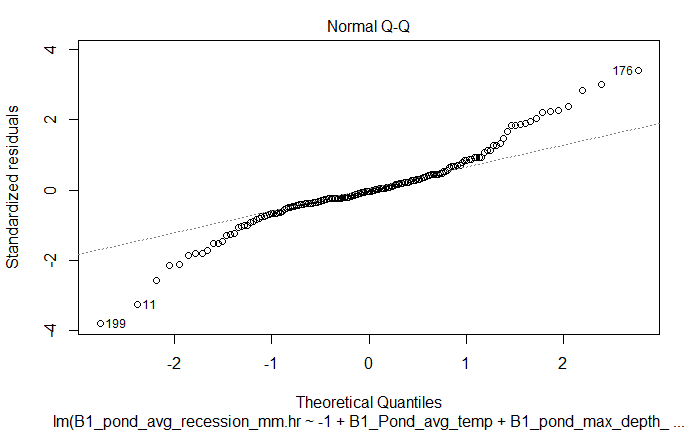
\includegraphics[width=\textwidth]{gfx/chapter-data-analysis/pond_recession_regression_normal_qq.png}
	\caption{Normal Q-Q plot for ponding recession regression.}
	\label{fig:pond-recession-regression-normal-qq}
\end{figure}

The regression model in Equation \ref{eq:pond-recession-regression} was chosen for its high R-squared value, which reflects the percent of variation in the response (recession rate) explained by the total variation in the model parameters, as well as its overall significance (high F-statistic with low p-value).
Parameters kept in the model (listed in Table \ref{table:pond-recession-regression}) have individual p-values < 0.05.
Estimates of recession rate predict the mean response for each unit change of the model parameters multiplied by their respective coefficients.
Other models considered included some combination of the final parameters, water temperature, event duration, and ordinal day.
While the equation predicts the mean response given a set of inputs and will not always be precise, a confidence interval of 95\%\ can indicate values that are outside the expected range.
Consecutive events with abnormally high or low recession values will indicate a need for inspection or intervention.

The model is not without its shortcomings, however, and does not account for departures from normality of the training data.
The Kendall seasonal trend statistic, $\tau$, tests for seasonal trends in monotonic, nonparametric data.
The $\tau$ statistic is a ratio of the probabilities of the observed order of the data to that of a different ordering.
That is, assuming two variables (X and Y, for example) are independent, the expected value of $\tau$ is 0, as the likelihood of the observed ordering is equal to that of any other ordering for two independent series \cite{Abdi2007}.
Calculating $\tau$ for comparison between B1 recession rate and the variables found in the regression equation \ref{eq:pond-recession-regression} results in the values found in Table \ref{table:kendall-test-results}.
All the relationships are significant enough to reject the claim that the pairwise comparisons are independent, suggesting the trends observed, and by extension their inclusion in a normal multiple regression, are significant, despite the lack of normality.

\begin{table}[ht!]
	\centering
	\caption{Kendall seasonal trend results.}
	\begin{tabular}{|l|l|l|}
		\hline
		Variable & Kendall $\tau$ & p-value \\
		\hline
		B1 pond mean temp (\degree C) & 0.122 & 0.001711 \\
		B1 pond max depth (mm)        & 0.915 & $<$2.2e-16 \\
		B1 ponding duration (hr)      & 0.829 & $<$2.2e-16 \\
		Total Rainfall (mm)           & 0.548 & $<$2.2e-16 \\
		Average Intensity (mm/hr)     & 0.410 & $<$2.2e-16 \\
		\hline
	\end{tabular}
	\label{table:kendall-test-results}
\end{table}

\subsection{Infiltration Drying Rate}

There are 76 valid events during the period of interest, essentially a subset of the standard events, quantified with different ending criteria to focus on soil moisture recovery.
For each event, the rate of drying for the three zones between the surface and the three soil moisture sensors at progressively deeper placements is calculated as distance/time.
Figures \ref{fig:drying-rate-pond-10}, \ref{fig:drying-rate-10-35}, and \ref{fig:drying-rate-35-60} demonstrate that this rate can be expected to fall within 0-5 cm per hour.
The 95\% percentile falls at 9.5 hours between 10 and 35cm (approx 2.63cm/hr), and 7.4 hours between 35 and 60cm (approx. 3.37cm/hr), meaning 95\% of events can be expected to exhibit drying rates faster than this.
The distribution does not display correlation with water temperature (Pearson correlation 0.047, p-value 0.34), and has remained consistent over time, as displayed in Figure \ref{fig:drying-rate-vs-time}.

The infiltration drying rate compares favorably to Saturo constant-head infiltration testing performed at the site across three growing seasons (repeat tests performed in downstream and upstream basins at discrete locations).
These tests showed a mean $K_{sat}$ value of 1.3-6.2 cm/hour, which compares favorably with the mean infiltration drying rate of 1.8-9.5 cm/hour.
Both metrics have large variances, and it would be helpful to do more direct comparison testing to investigate if the variability is consistent between them.

\section{Conclusions}
The methods described here attempt to evaluate methods for comparing storm events across time and space.
Using recession and infiltration KPIs to evaluate a system of GSI performance across an entire region will enable insights into long term design successes, and early detection of system errors.
The data have shown that performance is most highly impacted by temperature, which oscillates with an annual seasonal period.
GSI health can generally be quantified in terms of recession and drying rates for ponding level and soil moisture, respectively.
Higher rates for each quantify indicate faster transfer of water into the subterranean water table, and faster reduction in soil moisture that will lead to quicker preparation for the next storm.

In general, average recession rates between 40 and 120 mm/hr can be expected, depending on time of year and water temperature.
Average drying rates as high as 9.5 cm/hr can be expected, although this value would be expected to vary from GSI to GSI based on soil design criteria.
These statistics are not dependent on GSI parameters such as surface area, loading ratio, or number of inlets or outlets, and are therefore independent of site configuration.
The statistics can be calculated for any GSI system, or part of a system, to determine if infiltration rates and recovery rates fall within the expected range.
Thanks to the few parameters needed, namely ponding depth and soil moisture level, few sensors are necessary, keeping costs for this kind of monitoring low, making it accessible to be deployed at a larger number of sites, or at multiple locations within a single site.
While this work intentionally does not address spatial variability within a single site for infiltration or drying rates, the data collected are assumed to represent the average conditions throughout SMP~A, and the same assumption would be valid for the statistics calculated at other sites in a similar manner.

The recession and infiltration rates are affected by conditions both above and below the soil surface and provide an acceptable proxy for soil health.
The recession rate is shown to be affected by temperature and could be reduced by clogging of the soil surface or compaction of lower soil layers, leading to reduced rates.
Similarly, the infiltration drying rate is shown to be consistent across a wide variety of GSI conditions and could be adversely affected by changing soil properties that make the GSI function less efficiently.
The established relationships and expected values for each are useful as indicators for long term performance, and departures from expectations are cause for further investigation.

\begin{figure}[ht!]
	\centering
	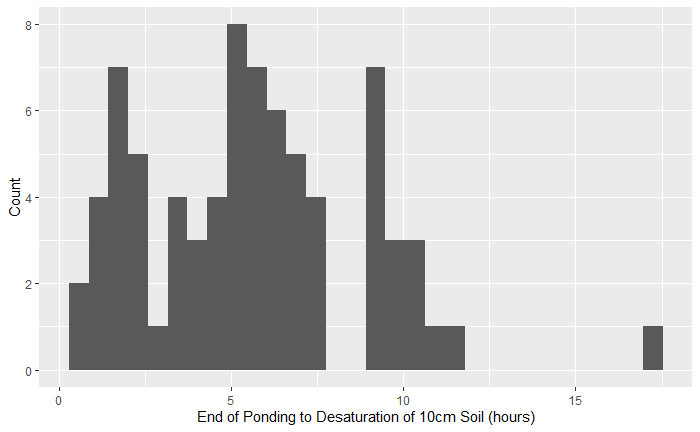
\includegraphics[width=\textwidth]{gfx/chapter-data-analysis/drying_rate_pond_10.png}
	\caption{Time to Desaturation from end of ponding to 10cm.}
	\label{fig:drying-rate-pond-10}
\end{figure}

\begin{figure}[ht!]
	\centering
	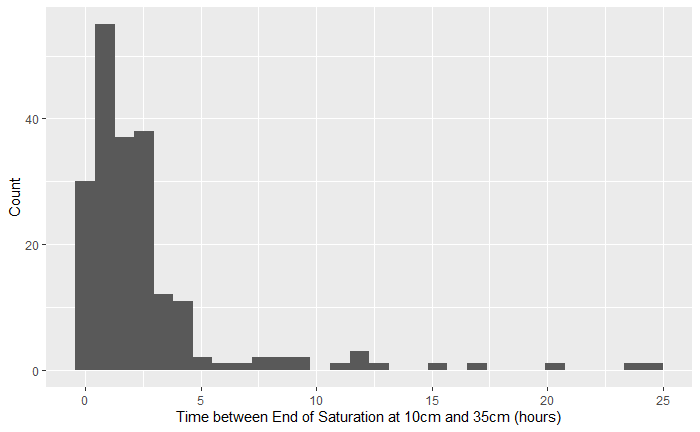
\includegraphics[width=\textwidth]{gfx/chapter-data-analysis/drying_rate_10_35.png}
	\caption{Time to Desaturation from 10 to 35cm.}
	\label{fig:drying-rate-10-35}
\end{figure}

\begin{figure}[ht!]
	\centering
	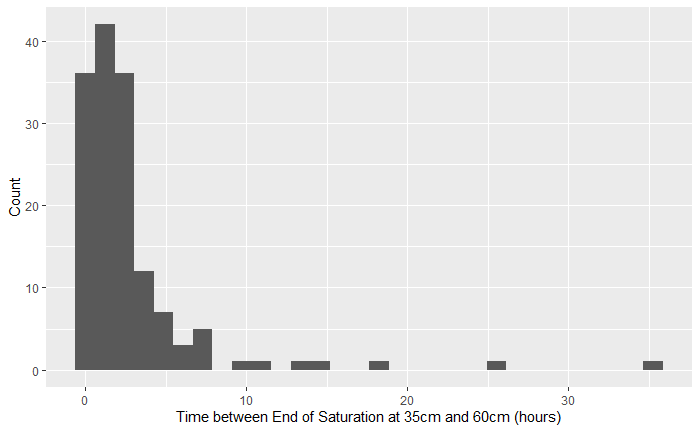
\includegraphics[width=\textwidth]{gfx/chapter-data-analysis/drying_rate_35_60.png}
	\caption{Time to Desaturation from 35 to 60cm.}
	\label{fig:drying-rate-35-60}
\end{figure}

\begin{figure}[ht]
	\centering
	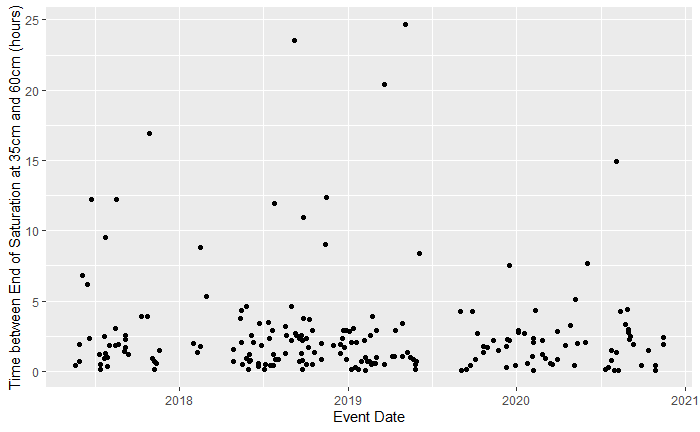
\includegraphics[width=\textwidth]{gfx/chapter-data-analysis/time_vs_drying_rate_10_35.png}
	\caption{Event Date vs Time to Desaturation from 10 to 35cm.}
	\label{fig:drying-rate-vs-time}
\end{figure}
% !TEX root = ../main.tex
%
\chapter{Conclusion}
\label{sec:conclusion}

This research work shows the benefits of a multi-faceted approach to long-term monitoring and analysis of GSI systems.
The integration of accurate data collection, robust data storage, and flexible yet relatable analysis methods across many sites has the potential to enable new insights into design and construction practices and reduce maintenance costs.
The work outlined herein lays the groundwork for carrying out long-term monitoring by addressing common instrumentation issues and potential solutions, describing a flexible framework for data storage, and preliminary work on data-driven performance indicators.

Ensuring that sensor equipment is well suited to conduct appropriate measurements and report valid data allows for an accurate, uninterrupted collection of data.
Understanding the intricacies of sensor configurations, communications, randomness of hydraulic characteristics, and opportunities for error helps mitigate invalid data.
Sensor, wiring schematic, and data logger choices should reflect these nuanced factors.
Digital communications significantly increase a sensor's ability to report valid data, ensuring that measurements taken in one location are correctly captured and stored by a physically separated data logger.
The increased confidence in data collected will enable future analysis of long-term trends, so investments and efforts made now in upgrading systems can have lasting benefits for GSI studies across all sites.
Furthermore, the improved data quality will free up researcher resources that can be focused on deriving insights and analyzing the data.

The FAIR principles are an easy check for data accessibility and make transferring analyses between sites simpler.
A flexible data format enables analyses that are easily scalable, since consistent metadata and controlled vocabulary are used across all sites.
This flexibility enables the expansion of the scope of research that is able to be conducted on larger GSI systems.
This is accomplished through controlled vocabulary for describing data and consistent, yet flexible, formatting of the database schema.
The long format of the main data table allows nearly infinite additional metadata combinations, meaning that future projects and sites will not require any updates to the schema.
This flexibility to add future sites is a key feature of the SIDM, as it enables long term studies to encompass both historical and future data easily in a single repository.
Future work to directly integrate monitoring equipment with the data ingestion process could mean that data becomes available in the SIDM almost instantaneously through the use of IoT protocols and methodologies, greatly expanding the value of consistent formatting and data descriptions.
The SIDM will unlock the potential for expanded collaboration between researchers and among project partners such as PennDOT and AECOM, better understandings of long-term monitoring results, and more robust analyses of multi-site GSI systems.

Lastly, the analyses outlined within are well suited to leveraging the data, as the results are consistent with labor intensive field and lab tests commonly accepted for infiltration capacity.
Recession and infiltration KPIs can be thought of as a proxy to these more complicated tests, such as the single and double ring infiltrometer or Saturo constant head tests, such that the long-term monitoring data is able to act as a substitute for routine GSI health checks.
The results of these health checks, which can be performed remotely by virtue of the connected monitoring network, can be used to determine the need for maintenance at a particular site or the need for more thorough inspection in cases of negatively trending performance.
The data have shown that performance is most highly impacted by temperature, which oscillates with an annual seasonal period.
This relationship is expected due to the change in water viscosity across the range of common temperatures in Philadelphia.
In general, GSI health is related to the recession and drying rates of the ponding level and soil moisture, respectively.
Both relationships are positive, such that higher rates indicate faster transmission of water through the engineered media layers and faster reduction in soil moisture leading to rapid recovery.
Results show that average recession rates between 40 and 120 mm/hr can be expected at the case study site, depending on time of year and water temperature.
Drying rate averages as high as 9.5 cm/hr over the course of a storm can be expected, although this value would be expected to vary between GSI systems based on soil design and pre-storm conditions.

These performance indicators are independent from GSI characteristics such as surface area, loading ratio, or number of inlets or outlets, and are therefore easily transferrable to other sites regardless of configuration.
The KPIs can be calculated for any GSI system, or part of a system, to determine if infiltration rates and recovery rates fall within the expected range, aiding in the design process by enabling feedback regarding target performance.
Few sensors are necessary for performing these analyses, namely a pressure transducer for ponding depth and a pair of soil moisture level sensors at a known separation distance, which helps keep costs for this kind of monitoring low.
The use of a consistent data format for a collection of GSI systems will allow these KPIs to provided up-to-date and at-a-glance information about the health of an entire system, making monitoring and managing maintenance requirements much more simple.
Therefore, implementing a basic monitoring network at many sites is economical, as robust data storage and analysis practices allow for data-driven decisions about allocation of maintenance and repair capital based on near real-time data, reduce wasted time and resources, and enable insight into long-term system-wide trends.

% --------------------------
% Back matter
% --------------------------
%
{%
\setstretch{1.1}
\renewcommand{\bibfont}{\normalfont\small}
\setlength{\biblabelsep}{0pt}
\setlength{\bibitemsep}{0.5\baselineskip plus 0.5\baselineskip}
\printbibliography{}
%\newrefcontext[labelprefix={@}]
%\printbibliography[heading=subbibliography,title={Webpages}]
}
\cleardoublepage

\appendix \cleardoublepage
% !TEX root = ../main.tex
%
\chapter{Appendix A}
\label{sec:appendix}
\nopagebreak
\begin{figure}[ht!]
	\centering
	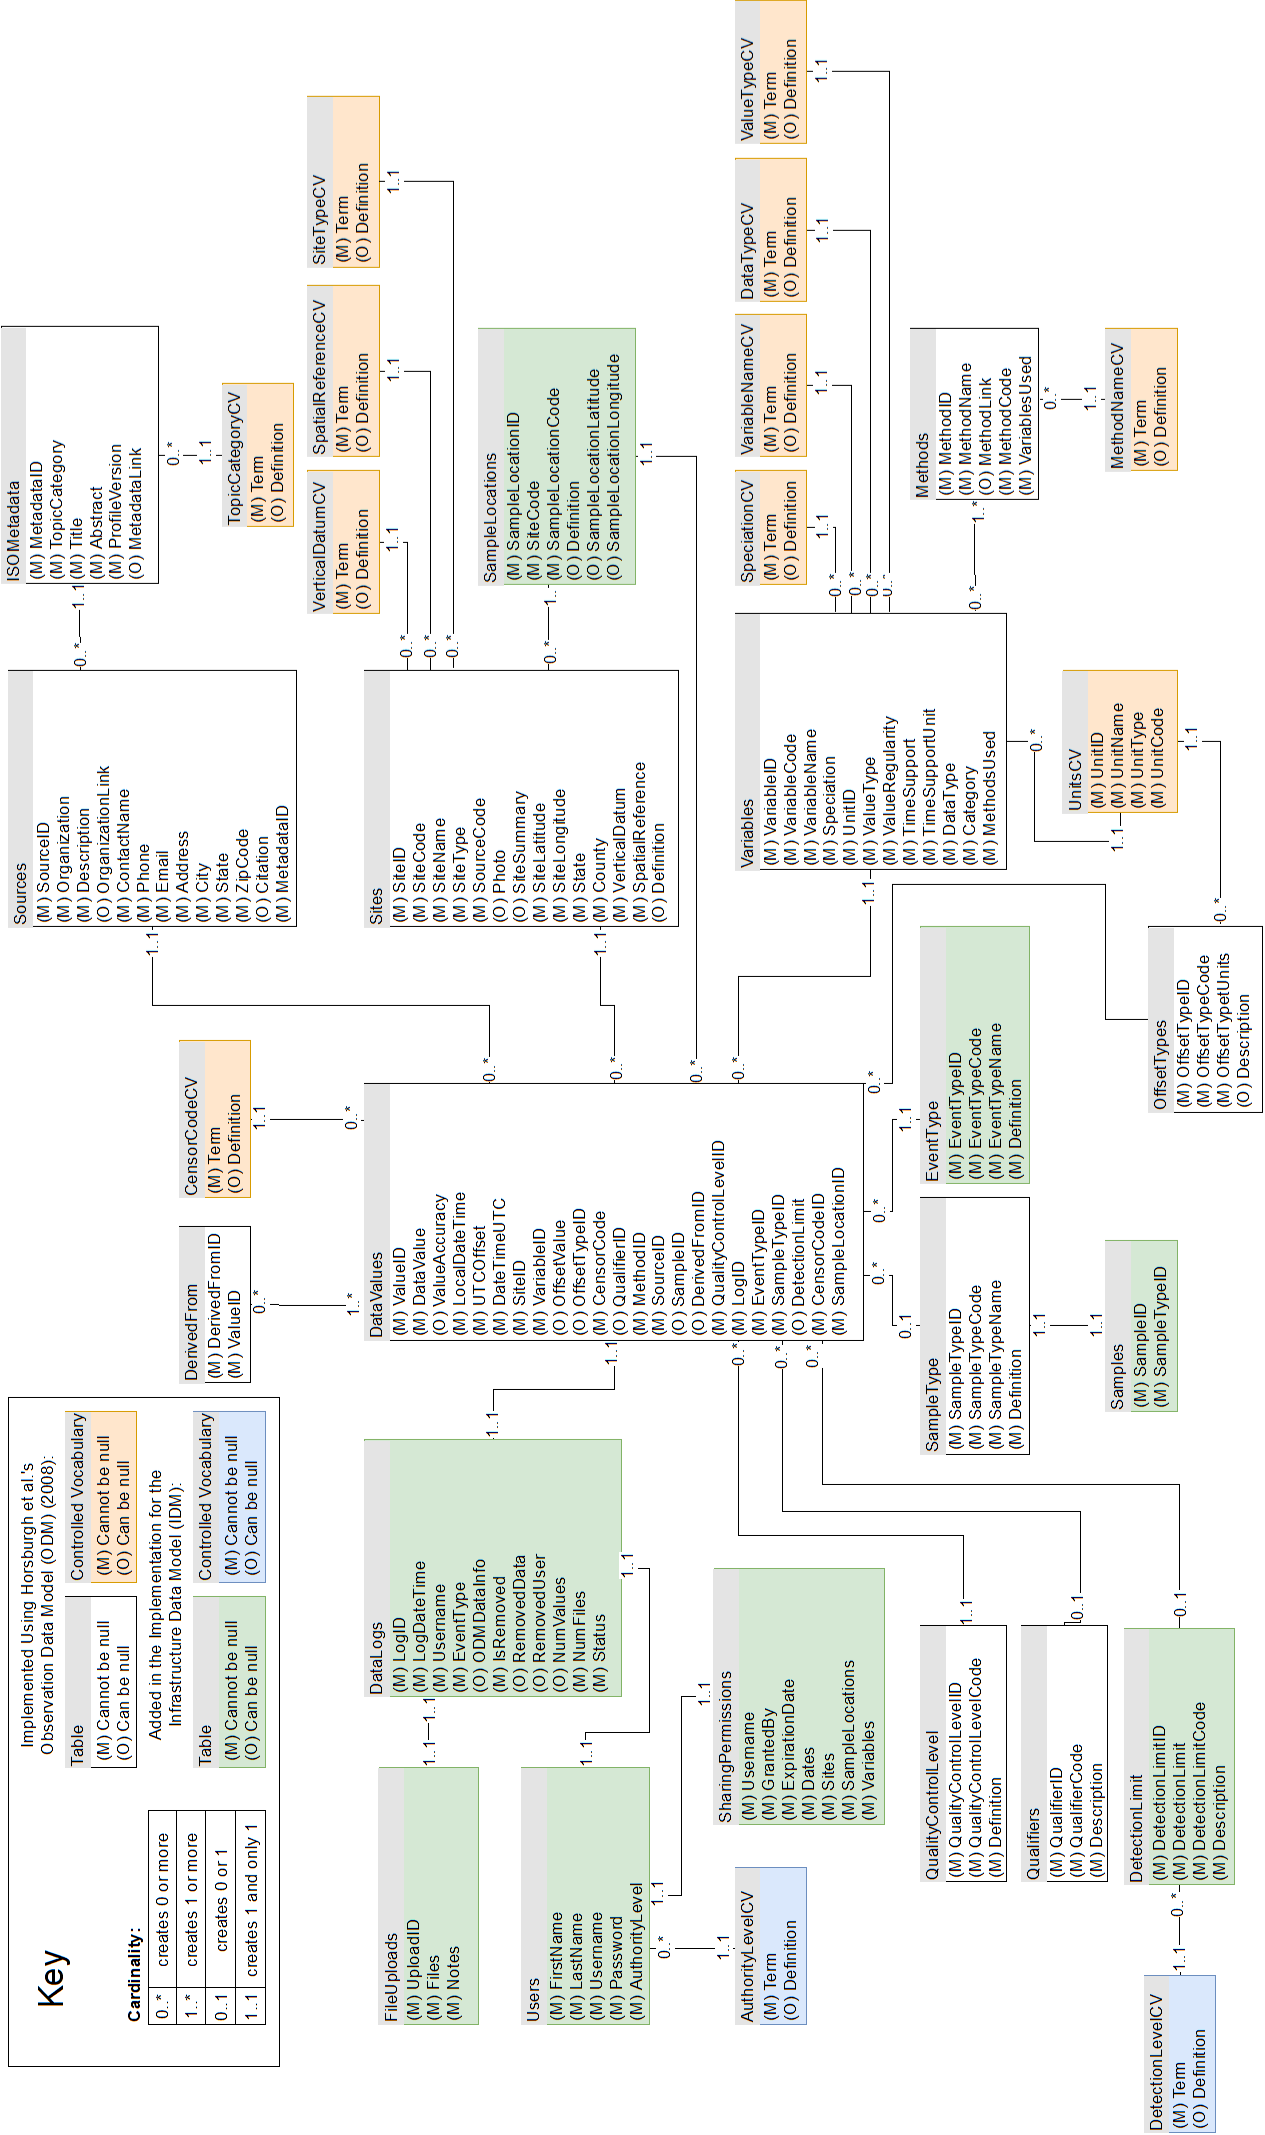
\includegraphics[width=\textwidth, height=0.9\textheight, keepaspectratio]{gfx/chapter-storage/idm_schema_tall.png}
	\caption[SIDM database schema.]{SIDM database schema (Smith et al., submitted).}
\end{figure}


\chapter{Appendix B}

The following R files are also available at \url{www.github.com/andrewkurzweil/MSCE-Thesis/R}.

Data ingest, cleaning, basic event statistics:

%\textit{NOTE: this file is the sole property of the Villanova Center for Resilient Systems and Pennsylvania Department of Transportation as used in monthly reporting. No permissions for outside use are granted and it is provided here for demonstration purposes only.}
\lstinputlisting[lastline = 799]{More-Code/PADOT_DATA_PRE-PROCESSOR_SMP_A.R}
\pagebreak

Ponding recession plots and regression modeling:
\lstinputlisting{../R/04 Recession Modelling.rmd}
\pagebreak

Infiltration timing plots:
\lstinputlisting{../R/05 Recession Timing.rmd}
       % INCLUDE: appendix

%\cleardoublepage
%% !TEX root = ../main.tex
%
%************************************************
% Declaration
%************************************************
\pdfbookmark[0]{Declaration}{Declaration}
\addchap{Declaration}
\label{sec:declaration}
\thispagestyle{empty}

I, \thesisName, hereby certify that this work is my own and has been completed with the assistance of only those sources listed herein.

\bigskip

\noindent\textit{\thesisUniversityCity, \thesisDate}

\smallskip

\begin{flushright}
	\begin{minipage}{5cm}
		\rule{\textwidth}{1pt}
		\centering\thesisName
	\end{minipage}
\end{flushright}

%*****************************************
%*****************************************


%\mbox{}

% **************************************************
% End of Document CONTENT
% **************************************************
\end{document}